\documentclass{article}

\usepackage{corl_2020} % Use this for the initial submission.
% \usepackage[final]{corl_2020} % Uncomment for the camera-ready ``final'' version.

% IEEE
% \documentclass[letterpaper, 10 pt, conference]{ieeeconf}  % Comment this line out if you need a4paper
%
% \IEEEoverridecommandlockouts                             
% \overrideIEEEmargins

\usepackage[utf8]{inputenc}
\usepackage[T1]{fontenc}
\usepackage{graphicx}
\usepackage{float}
\usepackage{xcolor}
\usepackage[normalem]{ulem}
\usepackage{subfig}

\usepackage{amsmath}
\usepackage{amsfonts}
\usepackage{amssymb}
\usepackage{mathtools}
\usepackage{todonotes}
\usepackage{enumitem}
\usepackage{multicol}
% \usepackage[noend]{algpseudocode} % this breaks my algorithm box

\usepackage{tikzpagenodes}

\usepackage{algorithm,algorithmic}

\newcommand{\ph}[1]{{\textbf{#1}:}} % paragraph header
% \newcommand{\todo}[1]{{\color{red} #1 }} % Tasks to do
\newcommand{\note}[1]{{\color{cyan} NOTE: #1 }}
\newcommand{\hn}[1]{{\color{orange} NOTE: (Henry) #1 }}
\newcommand{\gautam}[1]{{\color{cyan}Gautam: #1 }}
\newcommand{\argmax}{\mathop{\mathrm{argmax}}}
\newcommand{\argmin}{\mathop{\mathrm{argmin}}}

% IEEE
% \title{\LARGE \bf
% Perception-aware and Risk-cognizant Planning Under Uncertainty for Autonomy in Extreme Environments
% }

\title{
PLGRIM: 
Perception-aware and Risk-cognizant Planning Under Uncertainty for Autonomy in Extreme Environments
}
% PLGRIM (pilgrim): Planning at Local and Global levels with Robust Information Maps


% The \author macro works with any number of authors. There are two
% commands used to separate the names and addresses of multiple
% authors: \And and \AND.
%
% Using \And between authors leaves it to LaTeX to determine where to
% break the lines. Using \AND forces a line break at that point. So,
% if LaTeX puts 3 of 4 authors names on the first line, and the last
% on the second line, try using \AND instead of \And before the third
% author name.

% NOTE: authors will be visible only in the camera-ready (ie, when using the option 'final'). 
% 	For the initial submission the authors will be anonymized.

\author{
  Sung-Kyun Kim*\\
  NASA Jet Propulsion Laboratory\\
  California Institute of Technology\\
  United States\\
  \texttt{sung.kim@jpl.nasa.gov} \\
  \And
  Amanda Bouman*\\
  Department of Mechanical and Civil Engineering\\
  California Institute of Technology\\
  United States\\
  \texttt{abouman@caltech.edu} \\
  \And
  Gautam Salhotra\\
  Department of Computer Science\\
  University of Southern California\\
  United States\\
  \texttt{salhotra@usc.edu} \\
  \And
  David D. Fan\\
  NASA Jet Propulsion Laboratory\\
  California Institute of Technology\\
  United States\\
  \texttt{david.d.fan@jpl.nasa.gov} \\
  \And
  Kyohei Otsu\\
  NASA Jet Propulsion Laboratory\\
  California Institute of Technology\\
  United States\\
  \texttt{kyohei.otsu@jpl.nasa.gov} \\
  \And
  Joel Burdick\\
  Department of Mechanical and Civil Engineering\\
  California Institute of Technology\\
  United States\\
  \texttt{jwb@robotics.caltech.edu} \\
  \And
  Ali-akbar Agha-mohammadi\\
  NASA Jet Propulsion Laboratory\\
  California Institute of Technology\\
  United States\\
  \texttt{aliagha@jpl.nasa.gov} \\
}


\begin{document}
\maketitle

% IEEE
% % \thispagestyle{empty}
% % \pagestyle{empty}
% \pagestyle{plain}

\begin{abstract}
In order for robots to achieve a useful level of autonomy in novel environments, they must take into account uncertainties in localization, sensor measurements, and unknown hazards, as well as the effect of its own actions on these uncertainties.  Although there are many general methods for planning under uncertainty, we are interested in problems with very large scales, both in space (>10km$^2$) and in time (> 1 hour).  To make matters worse, we require computational efficiency and the ability to handle time constraints without severely impacting the optimality of the solution.  Towards this end we propose a unified framework for belief space planning that bridges the gap between high-fidelity information and traversability analyses and macro-level, discrete behavior planning.  We take samples of the belief space in order to construct a graph structure that encodes mission and environment-related information, which we call an Information Roadmap (IRM).  We demonstrate our framework in team CoSTAR's participation in the DARPA Subterranean Challenge, in which teams compete to autonomously search for artifacts in large, unknown, GPS-denied environments.
\gautam{Need to update. possible phrases: active learning, online planning, planning under uncertainty, learning value function in POMDP, MCTS, }
\end{abstract}

\gautam{PLGRIM (pilgrim): Planning at Local and Global levels with Robust Information Maps}
\gautam{Name suggestion: PLGRM: Planning at Local and Global levels with Road Maps. Pronounced pilgrim}

% Two or three meaningful keywords should be added here
\keywords{CoRL, Robots, Learning} 


% %%%%%%%%%%%%%%%%%%%%%%%%%%%%%%%%%%%%%%%%%%%%%%%%%%%%%%%%%%%%%%%%%%%%%%%%%%%%%%%%
% \section{Instructions}

% \ph{Paragraph header} Please start every single paragraph with a paragraph header, summarizing the intention of that paragraph. This is mainly for iterations during the paper preparation. We will remove most of them for the final report.

% {
% \color{orange}
% For the "notation consistency", please take a look at these works (note that the content might NOT be relevant, but notation could be useful)

% \begin{itemize}
% \item Feedback based IRM (for graph abstraction notation):
% FIRM: Sampling-based Feedback Motion Planning Under Motion Uncertainty and Imperfect Measurements (IJRR 2014)

% https://journals.sagepub.com/doi/10.1177/0278364913501564

% \item For 3D grid mapping with "information encoding"
% https://eric-heiden.com/publication/2019-crm-ijrr/

% \item For risk-aware local planning over confidence rich maps:
% https://eric-heiden.com/publication/2017-crm-to-iros/2017-crm-to-iros.pdf
% \end{itemize}


% }

%%%%%%%%%%%%%%%%%%%%%%%%%%%%%%%%%%%%%%%%%%%%%%%%%%%%%%%%%%%%%%%%%%%%%%%%%%%%%%%%

% Abstract
% 1 Introduction
% 2 Related work
% 3 Problem description/formulation
% -Coverage planning (SubT)
% -POMDP
% 4 Exploration-Coverage Planning Problem
% 5 Overall solution framework
% -Global/local IRM
% -Hierarchical planning
% -System overview
% 6 Algorithm description
% -(POMCP-based coverage planning)
% -Graph-level Planner
% -Lattice-level Planner
% 7 Experimental results
% -Simulation
% -Robot experiments
% 7 Conclusion
% Appendix



% INTRODUCTION

% coverage planning applications/significance

% highlight
% RL-based
% POMCP-based

% Our approach
% IRM structure for coverage planning
% -abstract graph/grid structure algorithm is agnostic to environment representation
% Using high-confidence generative model <--> risk map/traversability


% RELATED WORK

% Larger-space exploration
% : (Gautam) RL-based approaches
% <<Added to section 2>>

% -> limitations
% : (Amanda) TSP


% (Sung) POMDP solvers; purely model-based (given explicit/mathematical model)
% -> POMCP -> Model-based RL
% -> Challenge: even the generative model is not given!


% (David/Kyon)
% Traversability/riskmap --> model
% High-confidence gen model
% Traversabilty-aware ...



% SYSTEM DIAGRAM / Overall framework (Sung)




% STOCHASTICITY

% motion model: deterministic
% sensor model: 0/1 approximation (very simplified model)
% -noise; uncertainty; no information; 0 if out of FOV; out-of-FOV is fully stochastic (no information)

% partial observability (limited FOV)
% -> dependency on history
% -> POMDP


% TSP


% Reward function depends on history




% POMCP requires GT gen model.
% How to POMCP without GT gen model?
% -> need to estimate/construct *gen model* over time
% -> *gen model* needs motion model (occupancy/risk) and reward function (coverage, occupancy)
% -> construct *gen model* from riskmap and pose\_graph

% Use of uncertainty of motion model and reward function estimator?
% : motion and sensor model are deterministically approximated
% : we use uncertainty in reward function



% \ph{Sources of uncertainty} - Problem Description (Amanda)
% \begin{enumerate}
%     % given lcoal IRM as GT, uncertainty in POMDP problem
%     \item (within our prob formulation) Partial observation of local IRM (within FOV): uncertainty of complete state of IRM
%     -> coverage during forward simulation -> reward function
%     \item (we use this uncertainty as 0/1 model)
    
%     \item Actuator noise/uncertainty AKA controller errors
%     \item (we don't model this uncertainty for outcome state of gen, i.e., s')
%     \item (we use this uncertainty in reward/cost function)
    
%     % initial IRM generation, and generative model
%     \item Environment sensor uncertainty (main)
%     \item \,\, Coverage: if dist $<$ 5m from pose_graph, then P(cov) = 1, otherwise P(cov) = 0 (sub)
%     \item \,\, Occupancy: based on lidar sensor reading, ... (complex process of traversability analysis)
%     \item (we model this uncertainty as 0/1 model)
    
%     \item (NOTE: we do not assume localization error (robot pose))
% \end{enumerate}
% => Described these simplified modeling in experimental section


% It is not fundamentally impossible to do incremental planning?
% -> Fusion/accumulated/aggregated belief update for gen model construction? 
% -> keep track of riskmap(1:t) and pose_graph(1:t) -> gen_model at time t+1
% --> [FUTURE WORK] spatio-temporal memory of local IRM
%     REPRESENTATIONAL BENEFIT; placeholder of enriched information
% => Receding horizon control over stitched local IRM at (t-1) and (t)
% -> maybe a general problem for RHC approaches for exceptions!


% mathematical formulation

% $V(b) = ...$ (with GT gen)
% $\hat{V}(b) = \mathbb{E}_\theta ...$ (with estimated gen with prior $\theta$)



% Algorithm description (Gautam)
% \gautam{added to subsequent sections with lots of changes}
% 1. Hierarchical planning
% We have a planner at a higher level that represents the entire map as a simple bidirectional graph. This helps us keep a map of the entire world at a high level. It has explored nodes that are part of the graph and potentially explorable nodes that are one edge away. This is called the graph-level planner, and it leads us to potentially explorable frontiers.

% Once we read a node in the graph, we have another local planner that represents the world around it as an occupancy grid. This is the lattice-level planner. Each cell in the grid has a probability of occupancy and a boolean parameter isExplored (also known as coverage). In this local level, the robots goal is to explore all traversable parts of this local grid using a modified version of the POMCP algorithm.

% 2. High-confidence...? gen model


% 3. Coverage planning
% Custom rollout






%%%%%%%%%%%%%%%%%%%%%%%%%%%%%%%%%%%%%%%%%%%%%%%%%%%%%%%%%%%%%%%%%%%%%%%%%%%%%%%%
\section{Introduction}

\ph{High-level mission} Consider a large-scale coverage mission in a unknown environment. A robot tasked to explore and search a GPS-denied unknown area, (under given time constraints?). Creating a map of the environment, accurately predicting risks, and planning motions that can meet the coverage and time requirements are essential elements of an autonomy architecture needed to realize such a mission.  In such an architecture, quantifying and planning over uncertainty is essential for creating robust, intelligent, and optimal behaviors.

% \ph{An illustrative example} Consider the situation where a robot explores a corridor with two doorways leading to unknown areas.  The first doorway is narrow, but leads to a large, unexplored area, away from areas the robot has already explored.  The second doorway is wider and leads to what the robot can sense from a long range is a small room.  In order for the robot to make a good decision about which door to explore, it needs to take into account the uncertainty of its knowledge of each doorway, the risk involved in traversal, the time it takes to traverse, and the expected new information the robot hopes to gain in the future.  Furthermore, the robot should plan beyond the horizon of its current sensing range, and decide on the order in which to explore the doorways.  The robot will also need to update its plan at a high frequency should the situation change (e.g. due to dynamic obstacles, changing mission constraints, time limits, etc.) (see Figure \ref{fig:firstPage}).

\begin{figure}[t!]
  \centering
  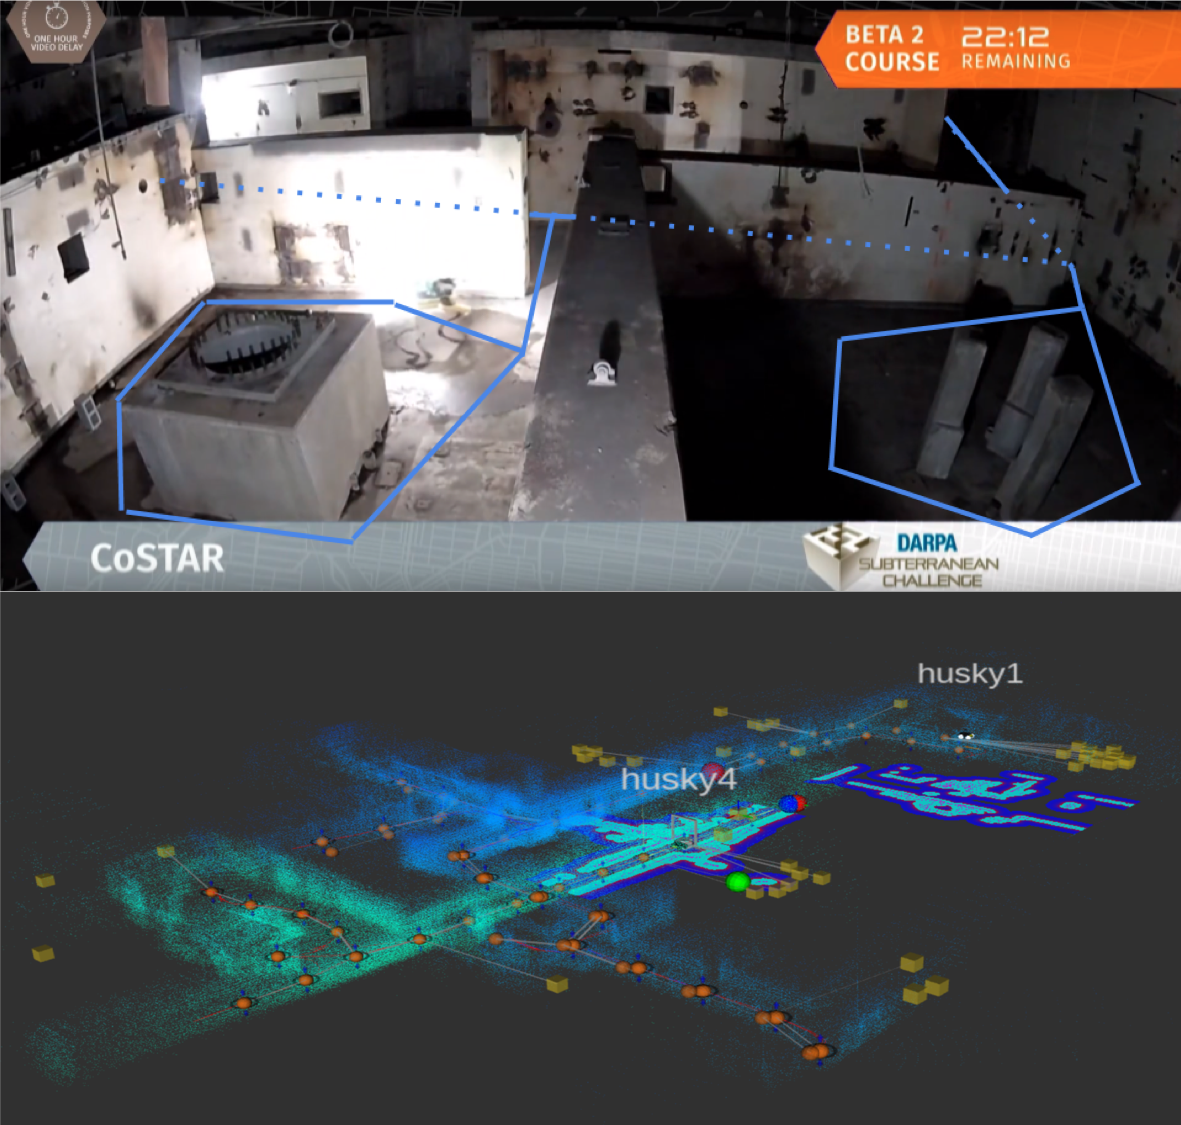
\includegraphics[width=.48\textwidth]{figures/firstpage_v2.png}
  \caption{The top figure shows a portion of the course in the Urban Circuit of the DARPA Subterranean Challenge. The blue line highlights two neighboring rooms joined by a narrow passage. CoSTAR efficiently explored both rooms by planning on the IRM. The bottom figure shows the IRM shared and maintained by multiple robots (husky 1 and 4 shown).}
  \label{fig:firstPage}
\end{figure}

\begin{figure}[t!]
  \centering
  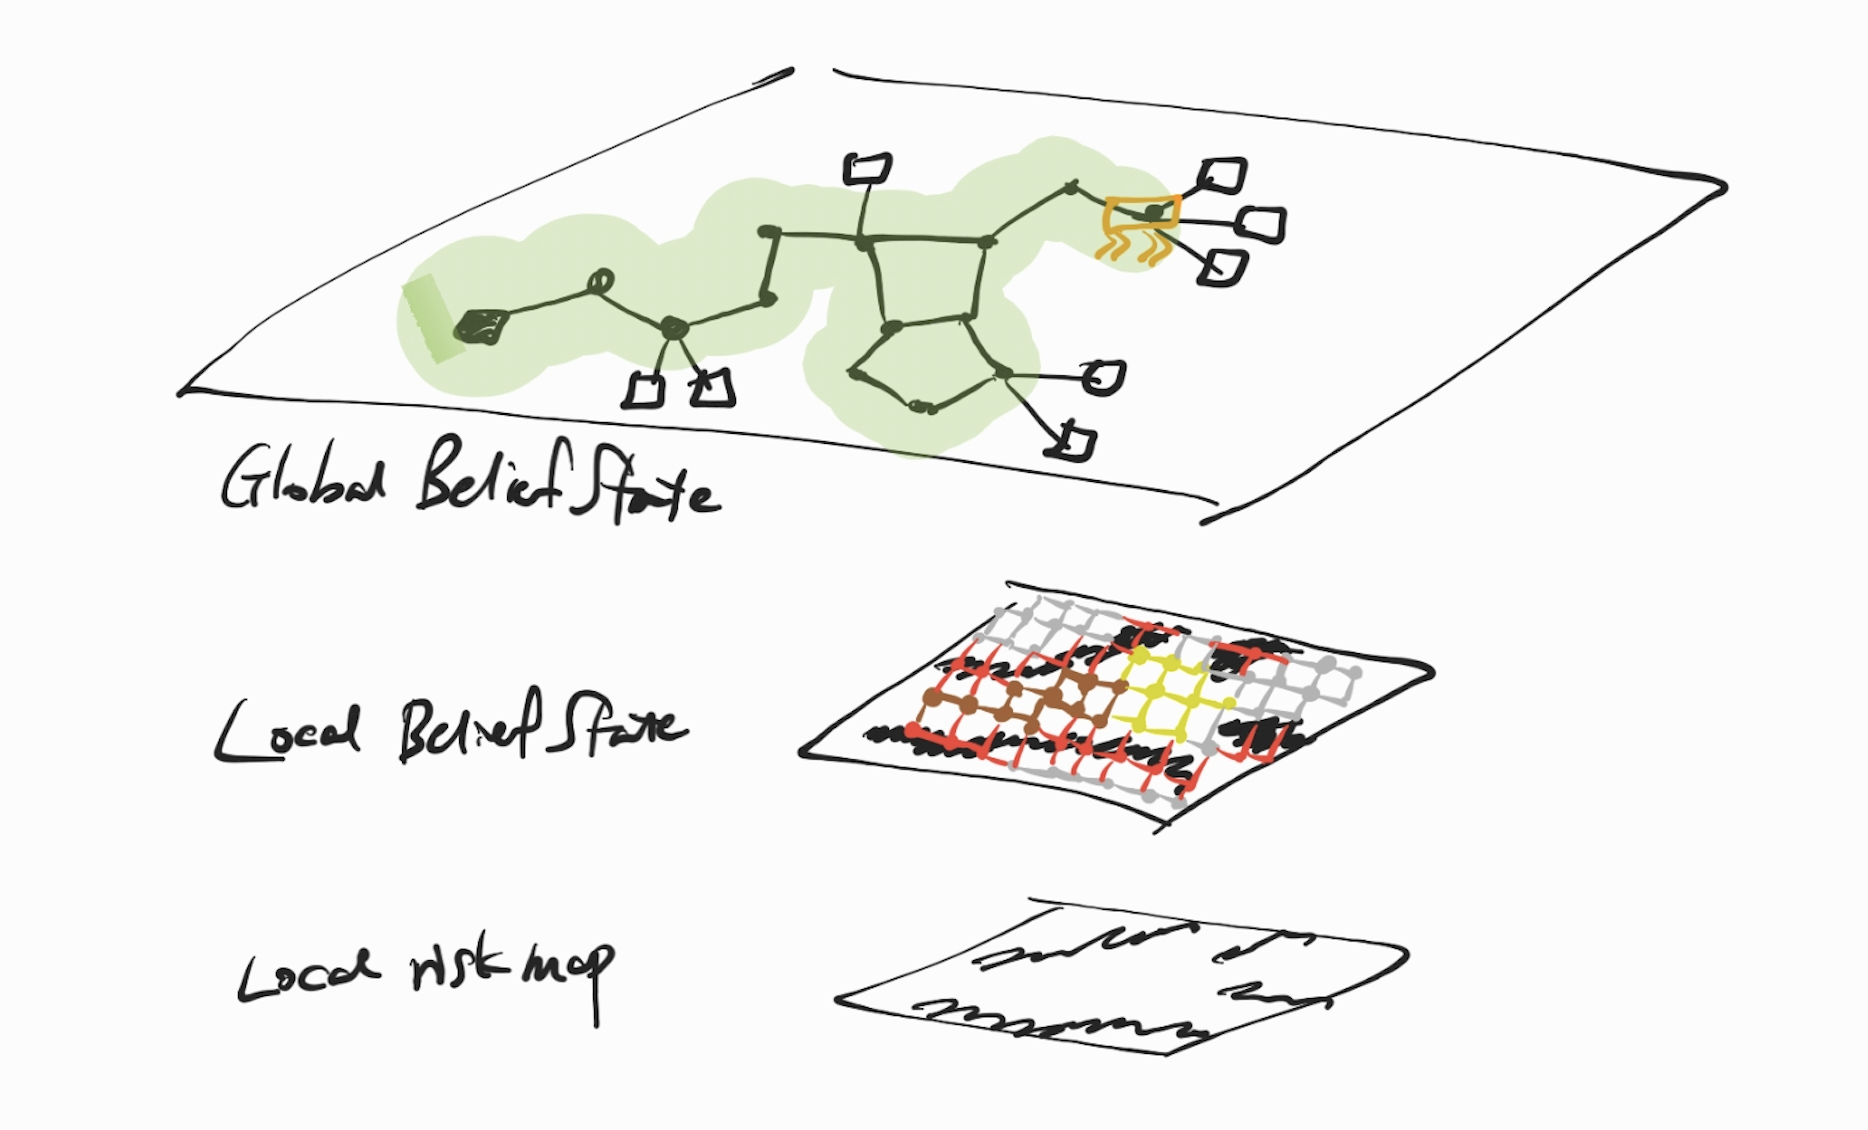
\includegraphics[width=.6\textwidth]{IRM_Planning/figures/sketch_hierarchical_belief_space.png}
  \caption{Illustration. [TODO] Visualize the planned path in each level.}
  \label{fig:illustration}
\end{figure}

% vertical 
% escape?
% IPE
% rviz
% DIAGRAM like Fig.~\ref{fig:architecture}

% \if 0
% The above-mentioned mission
% large-scale coverage in unknown space
% active learning under uncertainty
%
% two main challenges:
% 1) simultaneous optimization of information gathering and action cost; how to optimize this for a longer horizon?
% 2) high computational complexity for 1) with a long horizon; how to solve a large-scale problems?
%
% our contribution:
% 1) POMDP solver
%   a) long-horizon coverage planning with POMDP formulation 
%   b) with no access to the ground-truth generative model
%   => improved optimality in coverage in unknown space
% 2) Hierarchical structure
%   a) construct representation-rich abstract graph/roadmap at each hierarchical level
%   b) formalize POMDP planners to work on abstract graph representation
%   c) employ a hierarchical structure and connect the two levels of planner seamlessly
%   => solve larger coverage problems
% \fi


\ph{Problem description--learning perspective}
A coverage planning problem in a large-scale unknown space can be considered an active learning problem under uncertainty where the objective to find the best action sequence to maximize the accumulated reward over time.
As in the usual active learning setting, there are not many data points at start, and more data can only be collected once the selected action is executed.
Thus, the action selection should exploit the currently learned model (or belief) to maximize the rewards by efficient exploration.
Note that while the traditional active learning focuses on the exploration of the search space, this coverage problem needs to balance between exploration and exploitation since the robot operating under motion and sensing uncertainty is often safety-critical. 

\ph{Problem description--POMDP perspective}
From a different perspective, we can also cast this coverage problem as a Partially Observable Markov Decision Process (POMDP) problem. 
A POMDP is a principled formalization of sequential decision making process under motion and sensing uncertainty.
It employs the underlying intrinsic model of the sequential action-observation process under uncertainty, so that it can (asymptotically) converges to the optimal solution in a more sample-efficient manner than the model-free learning approaches.


---WORK-IN-PROGRESS---

two main challenges:
1) simultaneous optimization of information gathering and action cost; how to optimize this for a longer horizon?
2) high computational complexity for 1) with a long horizon; how to solve a large-scale problems?

our contribution:
1) POMDP solver
  a) long-horizon coverage planning with POMDP formulation 
  b) with no access to the ground-truth generative model
  => improved optimality in coverage in unknown space
2) Hierarchical structure
  a) construct representation-rich abstract graph/roadmap at each hierarchical level
  b) formalize POMDP planners to work on abstract graph representation
  c) employ a hierarchical structure and connect the two levels of planner seamlessly
  => solve larger coverage problems

% \ph{[WIP] Approach}
% Large-scale coverage in unknown space? Online, active learning problem!
% Probabilistic sequential decision making to maximize the average-case expected rewards by exploiting the current confidence about the environment at run time.
% (As in a receding horizon control fashion, it interleaves the decision making and action execution phases.
% At each decision making phase, it internally learns the value of each action sequence by interacting with the generative model of the system.
% Once a decision is made, it will execute the selected action and get another observation along with the actual reward.)

---OLDER TEXT---

\ph{Generic formulation}
The above-mentioned mission in its most general form can be cast as a POMDP, where the robot's belief of both its own position and the environment are a function of the history of the robot's actions and observations.  

\ph{Gap in the state-of-the-art}
In general, POMDPs suffer from the curse of dimensionality and are difficult to solve.  There are many algorithms for finding solutions POMDPs with varying degrees of efficiency and accuracy, and more continue to be developed today (\cite{silver2010monte,somani2013despot,bonet1998learning,kim2019pomhdp}).  However, because in our setting we aim to tackle problems which have large time horizons (>1 hour), large spatial extents (>10km$^2$), and high dimensional belief states (including beliefs on the state of the environment), determining a solution for the robot's behavior over the full belief becomes intractable.  Therefore, we introduce several key spatial and temporal discretizations which restrict the behavior of the robot to tractable search space.  This decomposition allows us to approximately solve the optimization in Eq. (\ref{eq:MDP-belief}) in a computationally tractable manner.

To obtain a tractable solution we discretize the belief space into a robot and task-relevant graph structure which reduces our search space for good policies, which we call an Information Roadmap (IRM).

\ph{Contributions}
In this work, we develop a framework for autonomous exploration of a large, unknown environment using a multi-resolution map representation enriched with future map estimates. We evaluate the expected perceptual information gain and traversability risk on a local dense map representation. This map is then discretized to achieve a global, computationally-efficient map representation, spanning the entirety of the known environment, and enriched with the locally gathered map estimates. High level actions are planned on the global map, and then converted to low level actions on dense map.    

\ph{Outline}
In the next section, we present the problem formulation. In Section \ref{sec:lattice_representation}, we describe our high-resolution representation of the environment (occupancy map). Section \ref{sec:planning} focuses on how we discretize the high-resolution map to achieve a low-resolution representation (graph) and how we plan robot action sequences on both the graph and map. Section \ref{sec:hierarchical} presents concrete details about how the graph and map planners interact in a hierarchical manner for autonomous exploration of large, unknown environments. Finally, in Section \ref{sec:urban}, we describe how we implemented this hierarchical planning scheme for the Urban Circuit of the DARPA Subterranean Challenge.

% \begin{figure}[t!]
%   \centering
%   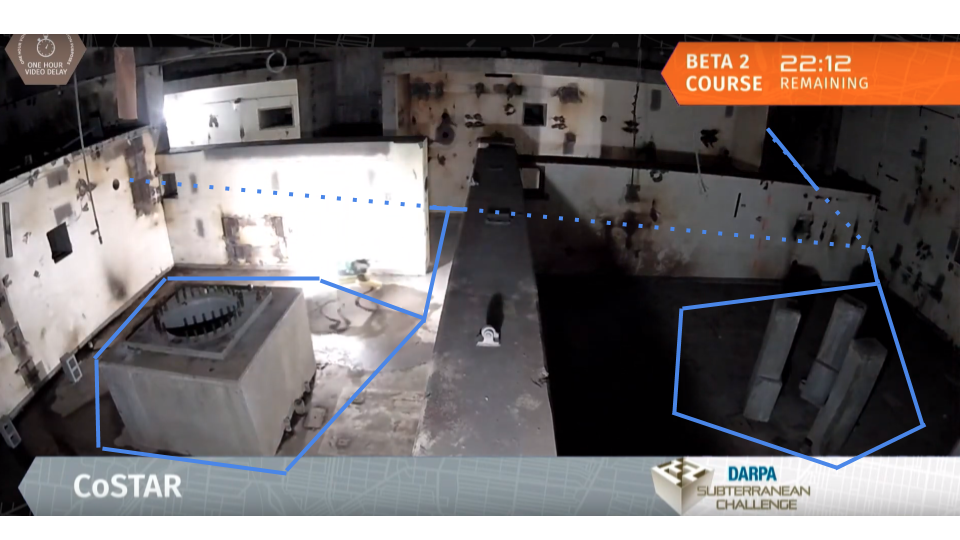
\includegraphics[width=.48\textwidth]{figures/FirstPage.png}
%   \caption{This figure shows one of the ... (most difficutl!) farthest rooms in the course in the lower level... CoSTAR was the only team able to reach this room .... using ... via narrow passages and ...}
%   \label{fig:firstPage}
% \end{figure}

%%%%%%%%%%%%%%%%%%%%%%%%%%%%%%%%%%%%%%%%%%%%%%%%%%%%%%%%%%%%%%%%%%%%%%%%%%%%%%%%
\section{Related Work}

\ph{General}
Numerous approaches have been proposed to solve exploration problems in very different domains.

\ph{Coverage--Frontier-based exploration}
Frontier-based exploration is a widely used approach for autonomous exploration \cite{yamauchi1997frontier,tao2007motion,keidar2012robot,heng2015efficient}.
This approach has two main processes: detection/pruning of frontiers and navigation to the best frontier.
Frontiers encapsulate the spatial information about the border of unknown and known spaces, and navigating to a frontier makes the robot to explore the unknown space.
A similar variant is the Next-Best-View algorithm that considers the range sensor footprint after one future steps and evaluates the next best action. \cite{gonzalez2002navigation,grabowski2003autonomous}
%
By keeping the exploration until exhausting all the remaining frontiers, this approach can guarantee \textit{completeness} of the coverage of the reachable spaces.
However, it follows a one-step look-ahead greedy policy by selecting the best frontier upfront.
Thus, it is highly subject to local minima (i.e., not being able to make any progress in coverage over time) and can cause significant suboptimality.

% The limitations of those approaches are
% 1) This approach can guarantee completeness of coverage, but no notion of optimality (one-step look-ahead greedy policy)
% 2) Challenges in large-scale exploration


\ph{Coverage--(Model-free) RL-based approaches}
Reinforcement Learning (RL) has been applied to solve exploration by using rewards internal to the agent. \citet{pathak_icm} proposed an Intrinsic Curiosity Module which is formulated with 'surprise'; the more difference between your predicted and actual states, the more the internal curiosity reward of the agent. This can fail in certain situations. The most popular experiment on this was from \cite{burda2018study}, where an agent is dropped in an environment where it can move but also change channels on a TV (if it is near the TV). The agent would just be drawn to the TV because changing the channels constantly gave it a new visual reward and it wouldn't explore the rest of the map. This was known as a 'couch-potato' behaviour of the exploratory agent. Thus, the agent was curious, in a sense, but not productive in exploring the map.

\citet{ECR2018} proposed agents that mark parts of the map as 'far away' in an effort to deincentivize single-step jumps such as changing a TV channel. These agents go through the environment and are only rewarded for observations that are relatively far away from the current observation. While this is a potential solution for the couch-potato effect, we now need to track potential landmarks where the agent has been to keep track of which parts are already explored. But there is no such memory for the agent. Instead the environment stores the list visited landmarks and gives the agent an augmented reward based on proximity to currently explored landmarks.

More recent work on random network distillation \cite{rnd} incentivizes exploration into unfamiliar territory by rewarding prediction of the output of a fixed random neural network in visited states. This has shown to help in hard-exploration Atari games like Montezuma's revenge.

[MESSAGE] From the decision making perspectives, the RL-based approach is also myopic one-step reward maximization, which may result in suboptimality in the global sense.


\ph{Coverage--(Model-based RL) POMDP approaches}
% POMCP using MCTS; model-based RL approach with POMDP formulation
%
A POMDP-based approach enables finding a non-myopic policy in a formal decision theory framework.
A POMDP solver considers long-horizon action sequences, interactively learns the value function of each, and returns the best action sequence that maximizes the accumulated rewards.
While there is an intrinsic challenge in the computational complexity, this approach has its own strength in simultaneous handling of both actions and observations for sequential decision making.

In unknown-space exploration domains, several techniques have been applied in POMDP formulation to reduce the problem complexity.
Gaussian belief assumption direct policy search scheme are employed in \cite{martinez2009bayesian} and \cite{indelman2015planning}.
\citet{Lauri2016planning} extended this to non-Gaussian belief modeling based on POMCP (Partially Observable Monte-Carlo Planning) \cite{silver2010monte} algorithm that uses particle filtering a Monte-Carlo Tree Search.
It also used the direct policy search approach to generate possible action sequences with a Gaussian kernel.
Still with such techniques for approximation the POMDP-based approach does not scale well due to the curse of history \cite{Pineau03}.

% Decentralized MCTS for team orienteering problem \cite{bestproblem2019dec}
% Cannot scale well with the belief space size... (local planning only)
% (for a fixed number of the robots in the case of Dec-MCTS)


\ph{[NOT URGENT] TSP approaches?}
Given a graph, the objective of the covering salesman problem is to determine the minimum length Hamiltonian cycle through a subset of the graph nodes such that every node is within a pre-specified distance from the cycle.  



\ph{Large scale--Hierarchical approaches}

Hierarchical planning structures are to scale up the problem by employing multiple solvers running at different resolutions and associating them together.
This approach has also been applied to the exploration and coverage domains.
%
\citet{umari2017autonomous} applied the hierarchical structure to the frontier-based exploration, so that the higher level frontier exploration module can guide the lower level frontier exploration module.
In \cite{dang2019explore}, the lower level module is extended to a more sophisticated frontier selection algorithm considering the information gain along each path.
\citet{Lauri2016planning} replaced the lower level module by a POMDP-based planner, so that the local coverage performance can be improved via non-myopic planning.

In the POMDP area, several works also showed the benefits of hierarchical structure.
\citet{vien2015hierarchical} proposed a hierarchical POMCP framework and demonstrated it outperforms Bayesian model-based hierarchical RL approaches in some benchmarks.
In \cite{kim2019bi}, hierarchical online-offline POMDP solver is proposed for risk-aware navigation planning, and showed synergy in the performance from global- and local-level planners.



\ph{Field-hardened--Traversability/risk-aware planning}
@David



%%%%%%%%%%%%%%%%%%%%%%%%%%%%%%%%%%%%%%%%%%%%%%%%%%%%%%%%%%%%%%%%%%%%%%%%%%%%%%%%
\section{Basic POMDP Formulation}

\ph{Structure} A POMDP is described as a tuple $\langle \mathbb{S}, \mathbb{A}, \mathbb{Z}, T, O, R \rangle$, where $\mathbb{S}$ is the set of states of the world, $\mathbb{A}$ is the set of actions, and $\mathbb{Z}$ is the set of observations sensed by the agent of the world. At every time step, the agent performs an action $a \in \mathbb{A}$ in state $s$ and receives an observation $z \in \mathbb{Z}$ resulting from the agent's perceptual interaction with the environment. The motion model $T(s, a, s') = P(s'\,|\,s, a)$ defines the probability of being at state $s'$ after taking an action $a$ in state $s$. The observation model $O(s, a, z) = P(z\,|\,s, a)$ is the probability of receiving observation $z$ after taking action $a$ in state $s$. Finally, the reward function $R(s,a)$ returns the expected utility for executing action $a$ in state $s$.

\ph{Belief State} Since the state of the world is not fully observable, the agent maintains a belief state $b_t\in \mathbb{B}$ defined as the posterior distribution over all possible states conditioned on past actions and observations at time $t$. The belief over state $s$ is $b_{t} = P(s \,|\, a_{0:t-1}, z_{1:t})$. After the agent executes action $a_{t-1}$ and receives observation $z_t$, the belief state can be updated according to Bayes algorithm:
\begin{align}
  b_t(s') &= \tau (b_{t-1}, a_{t-1}, z_t) \\
%   &= P(s' | a_{t-1}, z_t, b_{t-1}) \\
%   &= \eta \, P(z_t | s', a_{t-1}, b_{t-1}) P(s' | a_{t-1}, b_{t-1}) \\
%   &= \eta \, P(z_t | s', a_{t-1})  \sum_{s \in \mathbb{S}} P(s' | a_{t-1}, b_{t-1}, s) P(s | a_{t-1}, b_{t-1}) \\
  &= \eta \, O(s', a_{t-1}, z_t) \sum_{s \in \mathbb{S}} T(s, a_{t-1}, s') b_{t-1}(s)
  \label{eq:belief_update}
\end{align}
where $\tau$ is the state-transition function, and $\eta$ is a normalizing constant independent of state $s'$. 


\ph{Optimal Policy} A policy $\pi : \mathbb{B} \rightarrow \mathbb{A}$ maps each belief state $b$ to an action $a$. To compute the optimal policy, we rely on the one-step reward function $R(b_t, a_t)$ that encodes the desired behavior of the robot. The optimal policy maximizes the expected discounted sum of future reward for any given belief state:
\begin{align}
%   \pi^*(b) &= \arg\max_\pi \, \mathbb{E} \left[ \sum_{t=0}^{\infty} \gamma^t R(b_t, \pi(b_t)) \right] \\
  \pi^*(b) &= \arg\max_\pi \, \mathbb{E} \left[ \sum_{t=0}^{L} \gamma^t r(b_t, \pi(b_t)) \right]
  \label{eq:optimal_policy}
\end{align}
where $\gamma \in (0,1)$ is a discount factor which ensures that immediate rewards have a greater effect on decisions than future rewards. The overall objective is to solve this optimization problem in a computationally tractable way.





%%%%%%%%%%%%%%%%%%%%%%%%%%%%%%%%%%%%%%%%%%%%%%%%%%%%%%%%%%%%%%%%%%%%%%%%%%%%%%%%
\section{Problem Description: Coverage of Unknown Environment}

FORMAL DESCRIPTION, MORE SYMBOLS

% (intro) solve as POMDP so we can account for uncertainty in map
% (Q1 in sec4) computation challenge
% (Answer in sec5) Is hierarchical because POMDP is too hard to solve for large environment over large time scales
% (Q2 in sec4) coverage in unknown
% (A2 in sec5)

\ph{stodchast blind TCP} 

Stochastic Blind Covering Salesman Problem \\

%\ph{Problem} The traditional coverage problem is to find a trajectory that passes through all points in the a free space of a domain. %6
Given a pre-konwn discrete space $X$, the aim of the traditional coverage problem is to find a trajectory $\sigma$ that passes through all ....  free space $X_{free}\subset X$. 
%We can generalize this problem to one where the objective is to determine a path through a subset of the points such that every point in the domain is observable from the path.
We extend this definition to sensor-based coverage in 
continuous spaces (SCCS), where the objective is to determine a path through a subset of the space such that sensor FOV $F$ along the path covers the space, i.e., $\cup F_k = X$ % every point in the domain is observable from the path. %6

In this paper, we introduce and address teh  more general progelm of 
Time-constraint cvonering salmesan problem (TCCS), where 

The coverage problem is further complicated when a time constraint is applied and the domain is not known a priori, resulting in two competing objectives: the need to cover the known area and the need to explore in order to reveal the unknown area. % 3
% The coverage problem is further complicated when a time constraint is applied and the domain is not known a priori, resulting in two competing objectives: the need to cover the known area and the need to explore in order to reveal the unknown area. % 3

\ph{Challenges wihte sbTCP} 

In our POMDP framework, the environment is only partially observable to the robot due to its limited FOV. In a receding horizon fashion, we can find paths that cover the known space very efficiently, and we design the reward function to balance complete coverage and exploration.

%\ph{Why POMDP}
Coverage of an unknown environment can be modeled as a POMDP where the agent maintains a belief about its environment and plans a sequence of actions with the ultimate goal of minimizing spatial uncertainty. By predicting how future sensor information and vehicle control will affect its world belief, the agent can make long-horizon, near-optimal decisions that are robust to environment uncertainty. 


\ph{Traditional Map Representation} The belief state for this coverage POMDP is $b = p(M, x)$ where $M$ is the map state and $x$ is the robot state. We model $M$ as an occupancy map composed of grid cells  $m = \{\textbf{m}_i\}$ where $\mathbf{m}_i$ is a random variable representing some state (i.e. occupancy, coverage) of the $i$-th cell. In order to compute the posterior probability $p(M | z_{1:t}, x_{1:t})$ of the whole map $M$, given the robot's measurements $z_{1:t}$ and trajectory $x_{1:t}$, the cell states are traditionally approximated as binary with full independence between them \cite{TBF05,elfes1990stochastic}. %6

\ph{sbtcp formualtion}

%\ph{Computational Challenges} 
Even with these approximations to the coverage belief state, solving Eq. (\ref{eq:optimal_policy}) is intractable because of 1) the high dimension of the belief state $b$, particularly with respect to the belief over the map $M$, and 2) the large timescale $L$, since the complexity of the search space grows exponentially with time. To obtain a tractable solution, we discretize both the belief space $b=p(M,x)$ as well as the planning fashion. 


\ph{high-level objective}
The objective are twofold: to approximate... and to solve...


\ph{no access to the ground-truth generative model}
POMCP \cite{silver2010monte} is based on a Monte Carlo Tree Search which employs a generative model (i.e., a black box simulator of POMDP) in order to eliminate the need for explicit probabilistic representations that account for motion and sensing uncertainty. During each simulation, the initial state is sampled from the state belief, and the generative model provides a sample of the successor state, observation, and reward by adding noise to the output of a ground-truth model. However, in unknown-space exploration domains, the true state of the world is not known, so an alternative generative model is employed which uses a posterior distribution of the state based upon the most recently gathered sensor data in receding horizon manner. 


% This substitution of the ground-truth prior with the most up-to-date belief imposes additional challenges when applying the POMDP formulation to unknown-space coverage domains BECAUSE..
% However, during unknown-space coverage planning, we don't have access to the true state of the world, thus we instead use the robot's true sensor measurements of its environment as our ground-truth model. 
% No access to GT, using prior
% But, what's the limitation from this approach?
% - not as accurate as GT
% - ...

%%%%%% CITATION ADDED %%%%%
%%%%%% take a look at this page for some explanation/terms in RL:
%%%%%% https://ieeexplore.ieee.org/iel7/6895053/6906581/06907423.pdf?casa_token=aQK6RIfQAL0AAAAA:yVuS-SLSxozba3B0sCXzxHqoBgxoPIb3jtY3VUaEvssDGtoWAN3P6i6QDlzNZ97A2DGVdsbQZg
% Why [up-to-date belief] as a [prior]? What is the [rational] behind it?
% - KWIK (know what it knows) heuristic/strategy \cite{li2011knows}
% - optimism in the face of uncertainty \cite{brafman2002r}



% The generative model in traditional POMCP requires a ground truth from which the state transition and observations are sampled from.   samples the state belief in order to estimate long-term reward for large and complex systems.   

% Even worse, ...

% A POMDP problem where its explicit or generative model is not available.
% Note POMCP \cite{silver2010monte} is a breakthrough that employed a generative model (i.e., a black box simulator) in POMDPs to eliminate the need for explicit mathematical models for motion and sensing under uncertainty.
% However, even POMCP algorithm requires access to the ground-truth generative model.

% ...

% Thus, this imposes additional challenges when applying the POMDP formulation to unknown-space coverage domains.



%%%%%%%%%%%%%%%%%%%%%%%%%%%%%%%%%%%%%%%%%%%%%%%%%%%%%%%%%%%%%%%%%%%%%%%%%%%%%%%%
\section{Hierarchical Coverage Planner POMDP Framework (NAME???)}

% HICP: Hierarchical Information-based Coverage Planner
% HIRP: Hierarchical Information Roadmap Planner
% HIEP: Hierarchical Information-based Exploration Planner
% HIPER: Hierarchical Information-based Planner for Exploration Robots


In this work, we propose a novel framework of hierarchical coverage planner in a POMDP setting.
% It has two key components, an abstract coverage planner and a hierarchical planning structure, which will be introduced in the following subsections in details.

The main contributions are in two-fold---an abstract coverage planner and a hierarchical planning structure, which will be introduced in the following subsections in details.


\subsection{Abstract Coverage Planner} 

% \begin{itemize}
%     \item Reward function: Information gain from gen(current\_state, action)
%     current\_state contains coverage, i) gen(state,action) gives the new robot pose (from traversability and occupancy), in turn ii) gen(state,action) provides new world (coverage) from ray tracing (from occupancy), and iii) gen(reward function) computes info gain from old and new coverages
%     \item Action cost (path length, risk)
%     \item Observation: information gain, pose
%     \item State: robot pose and (abstract) environment (coverage)
%     $s = (x, W) \in \mathbb{S}$
%     \item Environment: representation encoding traversability, occupancy, and coverage??
%     $W = (V, E)$, $v \in V = [node_feature_vector]$, $e \in E = [edge_feature_vector]$
%     node\_feature\_vector: node (spatial) pose, 
%     edge\_feature\_vector: connecting nodes by this edge, 
%     \item Generative model construction: need World representation traversability and occupancy (but not coverage)
% \end{itemize}

\ph{Key characteristics} 
% We present an abstract coverage planner formulated as a variant of the POMCP solver... 
% (POMDP + Abstract state representation)
% Maintains belief over the robot and world representation
%
We present an \textit{Abstract Coverage Planner} that solves for the sequential action selection for coverage in unknown environments, given an abstract environment representation. %2

It formulates the coverage problem under motion and sensing uncertainty in unknown environments as a POMDP problem, and finds the best action sequence through learning of the value function of each robot state and world coverage state pair in the abstract representation.

\ph{Advantage (POMDP)} \\
% (compared to frontier-based greedy exploration)
% \begin{itemize}
%     \item Longer-horizon planning
%     \item Receding horizon planning (interleaving planning and execution)
% \end{itemize}
%
As described, there are two key components: a POMDP-based motion planner and an abstract world representation.


\ph{Advantage of using an abstract representation} Environment representation is fundamental in the development of planning schemes for autonomous exploration-coverage tasks. This is particularly true in large, unstructured environments where a robot locally requires high-resolution environmental information so that it has the ability to plan agile motions through challenging terrains. At the same time, the robot must maintain a general understanding of the previously explored space so 1) it will not attempt to re-cover areas and 2) it can navigate to previously identified information-rich frontiers when it has covered all points within a neighborhood of its current location. 

Our proposed structure extends traditional environment representation in two key ways. First, it has the ability to store various spatial and temporal metrics about the environment in a computationally-efficient and environmentally-agnostic architecture. Second, multiple structure instances with varying dimensions, resolutions, and information-metrics can represent a single environment as these sub-structures have the ability to share information and help coordinate hierarchical robot tasks. By encoding the map with multi-dimensional information at various resolutions, multi-objective planning algorithms can readily be implemented for complex environments.  


% (compared to concrete? representation)
% \begin{itemize}
%     \item Flexible and representation-rich format?
%     \item System-agnostic
%     \item Scalable
%     \item General cost functions (incorporate multiple objectives) -- IRM can encode multi-dimensional information feature vector (lidar, artifact1, artifact2, etc.)
%     \item coverage application -> spatial information + metadata (e.g. co2 sensor reading etc)
% so it extends to multi-dimensional information feature vectors
% \end{itemize}


\ph{Key/common components (Highlight)}
We present the following POMDP formulation for our proposed abstract information-rich map. In particular, we want to highlight the generative model $\hat{\mathcal{G}}$ which is constructed from the environment prior based on the robot's actual sensor measurements. 


% \begin{itemize}
%     \item Abstract state representation for coverage
%     \item Generative model construction from prior
% \end{itemize}



MOVE THESE TO PROBLEM DEFINITION/REPRESENTATION

\ph{System Representation} The system (robot + world) is represented by an abstract graph structure $W = (V, E)$, consisting of nodes $v \in V$ and edges $e \in E$.

% that captures the connectivity of the free space in the environment. We refer to this graph as the information roadmap (IRM) as its nodes $V$ and edges $E$ are enriched with environmental information. Each node $v \in V$ has attached to it a feature vector containing the probability $p(occ(v))$ that the node is occupied and the probability $p(cov(v))$ that the node was previously perceived by the robot's sensor suite $S$, constrained by viewing angle and distance. Each edge $e_{ij} \in E$ has attached to it a feature vector containing the probability $p(\rho(v_i,v_j)$) of traversal between the connected nodes $v_i$ and $v_j$.

\ph{State} We define the system (robot-world) state as a 2-tuple $s = (W, Q) \in \mathbb{S}$ consisting of the current abstract world representation $W$ and the node $Q \in V$ representing the robot state. The world can be further decomposed as $W = (W_{occ}, W_{cov})$ where $W_{occ}$ describes the geometry of the world and $W_{cov}$ encodes which regions of the world have been observed by the robot.   

\ph{Belief State} Our belief state is a 2-tuple $b = p(s) = p(W,Q)$ consisting of the partially observed world $W$ and the fully observed robot state $Q$.

\ph{Action} Given a node $v_i \in V$ in state $Q_i$ representing the robot's current position, a valid action at state $s$ is to move to connected node $v_j$ along the edge $e_{ij} \in E$. 

% $u(Q_i, Q_j) \in \mathbb{A}$
% where $u(Q_i)$ is a controller to drive the agent from $Q_i$ to $Q_j$.

% $Q.pos = V.pos$


% We define the graph-level policy $\pi^g \in \Pi^g$ as a function that returns a controller-specific parameter vector $\theta\in\Theta\subseteq\mathbb{R}^{n_\theta}$ given the current node $v \in V$.
% \begin{align}
%     \pi^g(v): V\rightarrow \Theta
% \end{align}
% For example, $\theta$ could represent the location of the next node to reach, specific gains for an LQR controller, weights of a neural network, etc.




\ph{Transition Model} Given an action $a$, the estimated transition model $T$ deterministically maps the robot and world state $s = (W, Q)$ to the subsequent state $s' = (W', Q')$:
\begin{align}
    % \hat{T}(s, a, s'; \, W_{occ,0}): \, \mathbb{S} \times \mathbb{A} \times \mathbb{S} \rightarrow \mathbb{S} \\
    \hat{T}(s, a, s'; \, W_{occ,0}): \, \mathbb{Q} \times \mathbb{W} \times \mathbb{A} \rightarrow \mathbb{Q} \times \mathbb{W}
\end{align}
where $W_{occ,0}$ represents the world geometry prior based on the robot's sensing of the real world. This geometry prior is used to estimate the traversability risk of an action $a \in \mathbb{A}$. If the traversabilty risk exceeds a pre-defined threshold, the robot does not transition along action-associated edge $e$ and, consequently, the state does not change: $s = s'$.

% $T: \mathbb{S} \times \mathbb{A} \times \mathbb{S} \rightarrow \mathbb{S}$ \\
%$T(s, a, s') = s \in \mathbb{S}$ 
% $\hat{T}(s, a, s'; W_{occ,0})$
% $T(s, a, s'; W_{occ,0})$

\ph{Observation} Upon taking an action $a$ in state $s$, the robot receives a complete observation of the robot state $Q$ and a partial observation of the world state $W$. Since we assume the uncertainty in the robot state $Q$ is fully captured in uncertainty in the world state $W$, we treat the robot state as fully observable. The world state $W$ is only partially revealed to the robot at any given time. Given a robot state $Q$, the robot observes only areas of the world within the field-of-view (FOV) of its sensors. Thus, we define the observation $z = w_{cov} \subset W_{cov}$ as the coverage state of the world within a sensor-constrained neighborhood of the robot. The estimated observation model is accordingly defined as:
\begin{align}
%   O: Q \times W \rightarrow \mathbb{Z} \\
%   O: Q \times W \xrightarrow{\text{sensor}} \mathbb{Z} \\
%   \hat{O}(s, a, z; \, W_{occ,0}, W_{cov,0}): \, Q \times W \xrightarrow{\text{sensor}} \mathbb{Z} \\
   \hat{O}(s, a, z; \, W_{occ,0}): \, \mathbb{Q} \times \mathbb{W} \xrightarrow{\text{sensor}} \mathbb{Z}
\end{align}
where $W_{occ,0}$ represents the world geometry prior based on the robot's sensing of the real world. This geometry prior is used to estimate neighborhood coverage $w_{cov}$ using ray-casting. While the world geometry $W_{occ,0}$ is known apriori, only by achieving a robot state $Q$ will the neighboring coverage status of the world be revealed.   

% $O: Q \times W \rightarrow \mathbb{Z}$. 
% $O: Q \times W \xrightarrow{\text{sensor}} \mathbb{Z}$. % where $S$ is one edge length.
% $\hat{O}(s, a, z; W_{occ,0}, W_{cov,0})$

\ph{Reward} The one-step estimated reward is computed as a function of the information gain and cost associated with an action:
\begin{align}
%   \hat{R}(s, a) = F(\text{info gain}(W_{cov}, z), \, \text{action penalty}(W_{occ}, a)): \, \mathbb{Q} \times  \mathbb{W} \times \mathbb{A} \rightarrow \mathbb{R} \\
    \hat{R}(s, a) = \mathcal{F}\Big[\, \textit{Info\_Gain}(W_{cov}, z), \; \textit{Cost}(W_{occ}, a) \, \Big]: \, \mathbb{Q} \times \mathbb{W} \times \mathbb{A} \rightarrow \mathbb{R} 
    % \hat{R}(s, a) = \mathcal{F}\Big[\, I(W_{cov}, z), \; C(W_{occ}, a) \, \Big]: \, \mathbb{Q} \times  \mathbb{W} \times \mathbb{A} \rightarrow \mathbb{R}
\end{align}
Information gain is defined as the marginal gain of information: $\textit{Info\_Gain}(W_{cov}, z) = I(W_{cov} \cup z) - I(W_{cov})$, as the benefit of being in a state $s$ is dependent on whether the robot has already observed neighboring areas in the world. The action cost can incorporate any robot behavior that increases exploration time. Action cost is a function of the world geometry $W_{occ}$ since this sub-state informs both the required actuator output (path length and velocity) and the proximity to the actuator's limitations (traversability risk) required to execute an action.

% $R: \mathbb{Q} \times \mathbb{W} \times \mathbb{A} \rightarrow \mathbb{R}$ \\
% $R(Q, W, a) = f(info_gain) - f(action_penalty)$
% $\hat{R}(s, a) = F(\text{info gain}(W_{cov}, z), \text{action penalty}(W_{occ}, a))$
% $R(s, z) = F(\text{info gain}, \text{action penalty})$
% $R(W_{cov}, W_{occ}, z, a) = F(\text{info gain}(W_{cov}, z), \text{action penalty}(W_{occ}, a))$

% We define the graph reward as the reward gained by executing the graph-level policy $\pi^g$ from node $v$ as a function $R^g(v, \pi^g): V \times \Pi^g \to \mathbb{R}$. The reward function, as defined in Eq. (\ref{eq:reward}), includes costs associated with path length and risk and utility associated with the observation $z$ of previously uncovered nodes.

\ph{Generative model} The estimated generative model simulates the robot's interaction with world and returns a successor state $s'$, observation $z$, and reward $r$ for a given state-action pair $(s,a)$:
\begin{align}
    \hat{\mathcal{G}}(\cdot) = \mathcal{F}(s, a; \, W_0) = \mathcal{F}\big[T(\cdot), O(\cdot), R(\cdot)\big]: \, \mathbb{S} \times \mathbb{A} \rightarrow \mathbb{S} \times \mathbb{Z} \times \mathbb{R} 
    % \hat{\mathcal{G}}(\cdot) = F(T(\cdot), O(\cdot), R(\cdot)) \\
    % \hat{\mathcal{G}}: Q \times W \times \mathbb{A} \rightarrow Q \times W \times \mathbb{Z} \times \mathbb{R} 
\end{align}
where $W_0 = (W_{cov,0}, W_{occ,0})$ is the world prior. 

% $\hat{\mathcal{G}} = F(b_0) = F(p(W_{occ, 0}))$, a prior belief $b_0$
% $\hat{\mathcal{G}}: \mathbb{S} \times \mathbb{A} \rightarrow \mathbb{S} \times \mathbb{Z} \times \mathbb{R}$
% $\hat{\mathcal{G}}(\cdot) = F(T(\cdot), O(\cdot), R(\cdot))$



% \ph{Policy} 

% General POMDP's policy (MAY NOT NEED THIS?)
% \begin{align}
%   \pi^*(b) &= \arg\max_\pi \, \mathbb{E} \left[ \sum_{t=0}^{L} \gamma^t R(b_t, \pi(b_t)) \right] \\
%   \label{eq:policy}
%   s.t.~&~\rho(b_t,\pi(b_t)) < \psi(t)
% \end{align}
% where $\gamma \in (0,1)$ is a discount factor which ensures that immediate rewards have a greater effect on decisions than future rewards. The acceptable risk threshold $\psi(t)$ is time-varying. As the duration of the mission progresses, the risk threshold $\psi(k)$ can increase to allow for riskier actions.

% We define the output of the graph policy $\pi^g(v_i)$ to be a neighboring node $\theta=v_j$, which is connected via a short path through free space. We assume that $\pi^{g}(v_i)$ induces a transition from nodes $v_i$ to $v_j$ with probability one:
% \begin{align}
%     T^{g} (v_i, \pi^g(v_i), v_j) = 1
% \end{align}
% There are a dynamic number of actions for a given node.



\subsection{Hierarchical Planning Structure} 
\ph{Intro} The proposed hierarchical planner decomposes the problem into tractable subproblems by introducing a spatial and temporal discretization which restricts the behavior of the robot to a smaller, information-efficient search space. The hierarchical planner has two layers with different environment representations. The higher layer, termed \emph{graph-level planner}, employs a sparse graph structure of dynamic size which spans the entirety of the known environment. The lower layer, termed \emph{lattice-level planner}, employs a dense grid structure of fixed dimensions which moves with the agent. 
% \textcolor{red}{(Sung) Yes, I think we can start using graph-level planner and lattice-level planner from this point. Otherwise, we need to explain the very similar relationship in Technical Details section again..}

\ph{Policy} The high level policy maps the high-level belief state $b^g$ to a controller specific parameter $\theta^l \in \Theta^l$ 
\begin{align}
    \pi^g : \mathbb{B}^g \to \mathbb{A}^g, \; \mathbb{A}^g = \Theta^l
\end{align}
The action space $\Theta^l$ encodes a global, non-myopic task, and serves as an input to the low level policy: 
\begin{align}
    \pi^l: \mathbb{B}^l \times \Theta^l \to \mathbb{A}^l
\end{align}
Output of low-level policy is some concrete controller to move robot.. so its considered myopic and constrained. We define an overall policy $\pi \in \Pi$ generated by combining the high-level policy $\pi^g$ and the low-level policy $\pi^l$:
\begin{align}
    % \pi(b) = \pi^l(b^l; \, \Theta^l) = \pi^l(b^l; \, \pi^g(b^g)): \, \mathbb{B}\rightarrow \mathbb{A} \\
    \pi(b) = \pi^l(b^l; \, \pi^g(b^g)) = \pi^l(b^l; \, \theta^l) : \, \mathbb{B}\rightarrow \mathbb{A} 
\end{align}

\ph{Reward} The one-step reward received by the agent upon taking a low-level policy $a^l$ in belief $b^l$ is:
\begin{align}
    r^l(b^l, a^l) = r^l(b^l, \pi^l(b^l; \theta^l) = r^l(b^l, \pi^l(b^l; \pi^g(b^g)))
\end{align}

\ph{Optimal policy/ global optimization objective} We define the optimal policy of the unified composite of the high and low level policy optimal policy as:
\begin{align}
  \pi^{*}(b) &= \arg\max_\pi \, \mathbb{E} \left[ \sum_{t=0}^{L} \gamma^t r^l(b^l_t, \pi^l(b^l_t; \pi^g(b^g_t)) \right]
  \label{eq:optimal_policy_unified}
\end{align}

\begin{align}
  \pi^{l*}(b) &= \arg\max_\pi \, \mathbb{E} \left[ \sum_{t=0}^{L} \gamma^t r^l(b^l_t, \pi^l(b^l_t; \theta^l) \right]
  \label{eq:optimal_policy_lattice}
\end{align}

\begin{align}
  \pi^{g*}(b) &= \arg\max_\pi \, \mathbb{E} \left[ \sum_{t=0}^{L} \gamma^t r^g(b^g_t, \pi^g(b^g_t)) \right]
  \label{eq:optimal_policy_graph}
\end{align}

$r^g(b^g, \theta^l)$ is (lower bound) approximation of $r^l(b^l, \pi^l(b^l; \theta^l))$.

At the high-level, we assume that $\pi^l$ is fixed and thus only optimize over $\pi^g$, which implies optimizing at the node-to-node level. However later we will show how we optimize over $\pi^l$ as well.

MESSAGE: Decomposed for tractability ...


%%%%%%%%%%%%%%%%%%%%%%%%%%%%%%%%%%%%%%%%%%%%%%%%%%%%%%%%%%%%%%%%%%%%%%%%%%%%%%%%
\section{Technical Details (better name?) Implementation?}

In this section we introduce the detailed description of our proposed framework.

\if 1 % COMMENTED
% at each time
HIERARCHICAL PLANNER

repeat\\
    (GLP)\\
    create IRM from pose-graph\\
    estimate generative model based on the current belief\\
    LLP-parameters \gets POMCP-GLP(Q^g, G^g, $\hat{\mathcal{G}}^g$)\\
    assign the LLP-parameters\\
    % if GLP planning\\
    %     create IRM\\
    %     estimate generative model based on the current belief\\
    %     call POMCP-GLP(Q^g, G^g, $\hat{\mathcal{G}}^g$)\\
    %     assign new LLP-parameters\\
    % else\\
    %     assign older LLP-parameters\\
    
    (LLP)\\
    read LLP-parameters from GLP (updated asynchronously)\\
    create low-level IRM\\
    estimate low-level generative model based on the current belief\\
    action \gets POMCP-LLP(Q^l, G^l, $\hat{\mathcal{G}}^l$)\\
    assign the action (control command/goal)\\

    (EXECUTIVE/CONTROLLER/SENSOR)\\
    execute the action\\
    get observation\\
    update robot state, costmap and pose-graph\\
until timeout


POMCP-*LP(Q, G, $\hat{\mathcal{G}}$)
\fi % COMMENTED




% \if 1 % COMMENTED



\subsection{Overall Framework} 



\begin{figure}[t!]
  \centering
  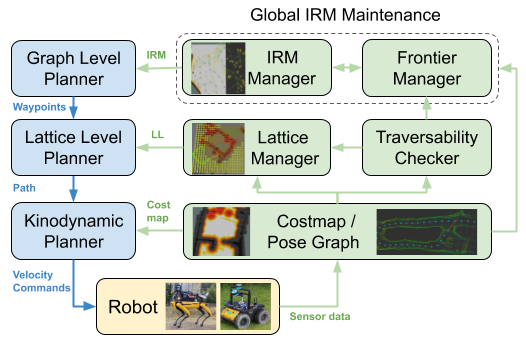
\includegraphics[width=.6\textwidth]{figures/SystemOverview.png}
  \caption{[WIP] System overview}
  \label{fig:system_overview}
\end{figure}

FIGURE: System Diagram
Input source to Graph-level Planner and Lattice-level Planner 
Connection between GLP and LLP
(move\_base)-level motion planner

% ?? NEED TO MENTION SLAM MODULE??


% See \url{https://docs.google.com/presentation/d/1DfS1T1_o_xenJ4o8x-9D0Uq-EO1xwyToqdSEE_V9eyU/edit#slide=id.g8cd3872972_2_0} for figure draft.


\subsection{Graph-Level Planner} 

% pseudo code

\ph{Environment Representation} We employ a sparse bidirectional graph structure $G^g = (V^g, E^g)$ that captures the connectivity of the free space in the environment. We refer to this graph as the information roadmap (IRM) as its nodes $V^g$ and edges $E^g$ are enriched with environmental information. Each node $v^g \in V^g$ has attached to it a feature vector containing the probability $p(occ(v^g))$ that the node is occupied and the probability $p(cov(v^g))$ that the node has been sensed by the robot. Likewise, each edge $e_{ij}^g \in E$ has attached to it a feature vector containing the probability $p(\rho(v_i^g, v_j^g)$) of traversal between the connected nodes $v_i^g$ and $v_j^g$.

\ph{State} Two-tuple $s^g=(G^g, Q^g) \in \mathbb{S}$ consisting of the current graph state $G^g$ and the robot state $q^g$ defined as the node closest to the robot's position. 

\ph{Graph action information reward}
We can approximate the graph action information reward $I^g(v, \pi^g)$ by the number of unknown cells within a 5m radius of the goal node $\pi^g(v_i)=v_j$.  This is an effective approximation when we assume a perfect sensor model which changes the probability of occupancy from 0.5 to either 1 or 0.  

\ph{Observation} The observation $z \in \mathbb{Z}$ received by the robot are the nodes directly connected to node $q_t$. The observation model is defined as $O: V^{cov} \times S \rightarrow \mathbb{Z}$ where $S$ is one edge length.

\ph{Action} Defined in "Abstract Planner"

\ph{Transition Model} We define the output of the graph policy $\pi^g(v_i^g)$ to be a neighboring node $v_j^g$, which is connected via a short path through free space. We assume that $\pi^{g}(v_i)$ induces a transition from nodes $v_i^g$ to $v_j^g$ with probability one:
\begin{align}
    T^{g} (v_i^g, \pi^g(v_i^g), v_j^g) = 1
    s.t.~&~\rho(b_t,\pi(b_t)) < \psi(t)
\end{align}

The acceptable risk threshold $\psi(t)$ is time-varying. As the duration of the mission progresses, the risk threshold $\psi(k)$ can increase to allow for riskier actions.

\ph{Observation}

\ph{Reward} We define the graph reward as the reward gained by executing the graph-level policy $\pi^g$ from node $v$ as a function $R^g(v, \pi^g): V \times \Pi^g \to \mathbb{R}$. The reward function, as defined in Eq. (\ref{eq:reward}), includes costs associated with path length and risk and utility associated with the observation $z$ of previously uncovered nodes. 

% The IRM graph grows through the addition of new nodes and edges as the robot navigates to previously unexplored areas of the map. We distinguish between two types of nodes: breadcrumb nodes and frontier nodes. Roughly speaking, breadcrumb nodes $b\in B \subset V$ encode the connectivity of free and traversable (low risk) space where the robot has previously explored, and frontier nodes $f\in F\subset V$ encode additional information about the value of exploring new locations, with $F\cup B = V$.

\subsection{Lattice-Level Planner} 

\ph{Environment Representation} We employ a rolling, fixed-sized lattice structure $G^\ell = (V^\ell, E^\ell)$ which is centered at the robot's current position. For ease of notation, we will drop the lattice notation for the remainder of this section. Each node object $v \in V$ has attached to it a feature vector containing the node position, probability of occupancy $p_{occ}(v)$, and probability $p_{cov}(v)$ that the node has been sensed by the robot. 

\ph{Risk} Each edge object $e \in E$ contains a risk value, or the probability of failing to safely traverse from node $v_i$ to connected node $v_j$:
\begin{align}
    \rho_{ij}(V; W_{occ}) = \mathcal{F} \big(v_i, \, v_j; \, p(W_{occ})\big)
\end{align}
where $W_{occ}$ encodes the 3D volumetric occupancy information acquired from raw sensor data. Within each grid cell $w_i \in W_{occ}$, there may exist multiple risk factors, due to a different source of potential failure, including rough terrain, proximity to obstacles, slope, slippery/muddy terrain. The number of risk factors is denoted by $n_\rho$. We compute the probability of failing to traverse a cell $\rho_c(w_i)$ as:
\begin{align}
    \rho_c(w_i) = 1-\prod_{r=1}^{n_\rho} (1-\rho_r(w_i))
\end{align}
We then compute the risk of the entire path from node $v_i$ to node $v_j$ as the aggregate risk of traversing the cells along the path:
\begin{align}
    \rho_{ij} = 1-\prod_t^{t+\tau}(1-\rho_c(w_{i_t}))
\end{align}


\ph{State} Two-tuple $s=(G, Q)  \in \mathbb{S}$ consisting of the current lattice state $G$ and robot state $V_q = (v_q, \dot{v}_q)$ where $v_q \in V$ is the node representing the robot's position and $\dot{v}_q$ is the robot's velocity. 

\ph{Observation} The estimated observation $z \in \mathbb{Z}$ consists of the nodes within line-of-sight of the robot node $v_q$, computed using ray-casting techniques on the prior occupancy map $W_{occ}$ in conjunction with sensor range constraints:
\begin{align}
    w_{cov} = \hat{O}(V, q; \, W_{occ,0}) 
\end{align}

\ph{Action} The output of the lattice policy is a control input $\vec{u}$ to the robot. 

\ph{Transition Model} We define the output of the lattice policy $\pi(v_i)$ to be a neighboring node $v_j$, which is connected by edge $e_{ij}$. We assume that $\pi(v_i)$ induces a transition from nodes $v_i$ to $v_j$ equal to the probability of traversal:
\begin{align}
    \hat{T}^{g} (v_i, \pi(v_i), v_j) = \begin{cases} 
    1-\rho_{ij} \; &\text{if $\rho_{ij} < \psi(t)$}\\
    0 \; &\text{otherwise}
    \end{cases}
\end{align}
The acceptable risk threshold $\psi(t)$ is time-varying. As the duration of the coverage mission progresses, the risk threshold $\psi(k)$ can increase to allow for riskier actions.

\ph{Information Gain} Entropy is a measure for the uncertainty of a posterior. The entropy $H_p(x) = E[-\log p(x)]$ is the expected information that $x$ contains if $x$ happens with probability distribution $p$. The posterior uncertainty of the lattice structure is:
\begin{align}
    H_{p_{cov}}(V) = -\sum_{v_i \in V}p_{cov}(v_i) \log p_{cov}(v_i) + \left(1-p_{cov}(v_i)) \log (1-p_{cov}(v_i)\right)
\end{align}
where $V$ is the set of nodes in the lattice, $v_i$ is the random variable associated with the $i$-th node, and $p_{cov}(v_i)$ is the probability that the node has been observed by the robot. The uncertainty reduction, or information gain, associated with an action $\pi(v_i)$ in belief $p_{cov}(V)$ is:
\begin{align}
    % I(\pi(v_i), w_{cov}) &= H_{p_{cov}}(V) - H_{p_{cov}}(V^\prime; \pi(v_i), w_{cov}) \\
    I(V; \pi(v_i), w_{cov}) &= \underbrace{H_{p_{cov}}(V)}_\text{current entropy} - \underbrace{H_{p_{cov}}(V^\prime; \pi(v_i), w_{cov})}_\text{future entropy}
\end{align}
where the second term represents the expected future entropy of the lattice when the agent observes $z = w_{cov}$ after executing action $\pi(v_i)$. The successor world state $p_{cov}(V^\prime)$ is computed according to Bayes' Algorithm (Eq. \ref{eq:belief_update}). 

\ph{Cost of Traversal} The cost of traversal associated with action $\pi(v_i)$ comprises risk, rotation, and traversal distance:
\begin{align}
    C(V; \pi(v_i), W_{occ}) = \alpha_{risk} \; \rho_{ij} + \alpha_{rot} \;  \cos^{-1}(\dot{\vec{v}}_q, \cdot \vec{u}) + \alpha_{dist} \; \vec{u}
    \label{eq:traversal_cost}
\end{align}
To account for the distance discrepancy between a lateral and diagonal action, we define $\alpha_{dist}=1$ if $\vec{u}$ is a multiple of $\pi/2$ (lateral action) and $\alpha_{dist}=\sqrt{2}$ (diagonal action) otherwise.

% (-pi, pi]
% [-135, -90, -45, 0, 45, 90, 135, 180]

% rotation penalty: $f(\dot{\vec{v}}_q, \vec{u}) = \cos^{-1}(\dot{\vec{v}}_q, \cdot \vec{u})$

% $Q^\ell = \{q, \dot{q}\}$
% $q \in \mathbb{V}$



\ph{Reward Function} The one-step estimated reward is a weighted sum of information gain and traversal cost:
\begin{align}
    % \hat{R}(s, a) : Q^L \times (W_{cov} \times \mathbb{Z}) \rightarrow \mathbb{R} \\
    \hat{R}(s, \pi(v_i)) = c_{I} I(V; \pi(v_i), w_{cov}) - c_{T}  C(V; \pi(v_i), W_{occ})
    \label{eq:lattice_reward}
    % \hat{R}(s, a) = c_{I} I(V; z) - c_{T} Cost()
\end{align}


\subsection{Algorithm: NAME?? PLGRM: Planning at Local and Global level with Road Maps}

Here we explain how the two instances of abstract coverage planners (graph-level and lattice-level planners) are combined and interact with each other in a unified framework...

Receding horizon control



\subsubsection{Global Level}
World represented as a graph. W = Simple bidirectional graph

$s^g = (Q^g, G^g)$. $G^g \sim W?$. Here, $Q^g$ = robot node $q \in V^g$ vertices  and $\dot{q}$ is velocity vector.

Generative model $\mathcal{G}$ is explained.

Rollout policy $\pi_{rollout}$ is random or Dijkstra-based to reach next unexplored node

Output of GLP is $\theta^l_t$, which gives a goal position to the robot executive (mobility service) to move the robot to an unexplored area of the map.

\subsubsection{Local Level}
World represented as a lattice. World W = dense lattice with occupancy information, similar to occupancy grid maps.

Gl = hyperlocal coverage information in the lattice (within robot FOV). Here, Qg = robot node $v_q$  and unit velocity vector $\dot{v}_q$. 

Generative model $\mathcal{G}$ is estimated from robot sensors. It assumes perfect motion model. It gives output $(s', o, r)$. Next state s' contains the new robot pose and velocity vector; . Observation o contains the occupancy information of lattice nodes within FOV of robot. r contains reward -- this includes fixed penalty for each step moved, distance penalty for moving along an edge, rotation penalty for change in robot velocity vector.

Rollout policy $\pi_{rollout}$ is Dijkstra-based to reach next unexplored node

Output of GLP is $a^{*l}_{t:T}$, which is a series of robot poses to reach, given to the robot executive.
\sout{\gautam{PUT SOME DESCRIPTION IN TEXT ABOUT THE ALGORITHM/FRAMEWORK}}

\subsubsection{Executive}
Describe mobility services here. What info does it need to move to a new position?

Goal position

cost/risk maps

other stuff?

% \textbf{Separate POMCP algorithm -- SIMULATE ROLLOUT SEARCH}



% Amanda/David Version
%%%%%%%%%%%%%%%%%%%%%%%%%%%%%%%%%%%%%%%%%%%%%%%%%%%%%%%%%%%%%%%%%%%%%%%%%%%%%%

\begin{algorithm}[t!]
\caption{Hierarchical Coverage Planner}
\label{alg:hierarchicalPlanner}
\begin{multicols}{2}
\begin{algorithmic}
\STATE \underbar{\textbf{Function HierarchicalPlan}}
\item \textbf{input: }Beliefs $b^g$, $b^l$ of states $s=(G, Q)$
\item \textbf{input: }World configuration $W$
% \item \textbf{input: }Optional rollout policy $\pi_{rollout}$
\REPEAT
    \STATE \textbf{\# Global level planner}
    \item  Obtain world information map
    \item Estimate $\hat{\mathcal{G}}^g$
    \item $\theta^l_{t:T} \gets \textsc{POMCP}(b^g, \hat{\mathcal{G}^g}, \pi_{rollout})$
    \STATE \textbf{\# Low level planner}
    \item Obtain local information map
    \item Estimate $\hat{\mathcal{G}}^l$
    \item $a_{t:T}^{*l} \gets \textsc{POMCP}(b^l;\hat{\mathcal{G}}^l, \theta^l_{t:T}, \pi_{rollout})$ 
    % \item \#learn value function and get best actions
    \STATE \textbf{\# Executive}
    \item Execute $a_{t:T}^{*l}$
    \item Obtain $z$ from sensors
    \item Update $Q$, $W$
\UNTIL timeout
\end{algorithmic}

\begin{algorithmic}
\STATE \underbar{\textbf{Function POMCP}}
\STATE \textbf{input: }Initial belief state $b_0$
\STATE \textbf{input: }Estimated generative model $\hat{\mathcal{G}}$
\STATE \textbf{input: }Optional rollout policy $\pi_{rollout}$
% \STATE
\STATE Initialize empty MCTS tree $T_r$
\REPEAT
    % \item Initial state $s_0 \sim b_0$
    \item \# Run SIMULATE with $\pi_{rollout}$ and $\hat{\mathcal{G}}$ to update $T_r$ with learned value function
    \item $T_r \gets \textsc{SIMULATE}(b_0; \hat{\mathcal{G}}, \pi_{rollout})$
    % \STATE Update the values and the number of visits by backpropagation from the leaf node to the root node
\UNTIL{timeout}
% \item 
\item Extract next N actions $a^*_{1:N}$ from $T_r$ \#N=1 for GLP. For LLP, keep going till leaf node
% \STATE
\RETURN $a*_{1:N}$
\STATE
\STATE
\STATE














% Gautam's Version
%%%%%%%%%%%%%%%%%%%%%%%%%%%%%%%%%%%%%%%%%%%%%%%%%%%%%%%%%%%%%%%%%%%%%%%%%%%%%%

% \begin{algorithm}[t!]
% \caption{Hierarchical Coverage Planner}
% \label{alg:hierarchicalPlanner}
% \begin{multicols}{2}
% \begin{algorithmic}
% \STATE \underbar{\textbf{Function HierarchicalPlan}}
% \item \textbf{input: }Beliefs $b^g$, $b^l$ of states $s=(G, Q)$
% \item \textbf{input: }World configuration $W$
% \item \textbf{input: }Optional rollout policy $\pi_{rollout}$
% \REPEAT
%     \STATE \textbf{\# Global level planner}
%     \item  Obtain world information map
%     \item Estimate $\hat{\mathcal{G}}^g$
%     \item $\theta^l_{t:T} \gets \textsc{POMCP}(b^g, \hat{\mathcal{G}^g}, \pi_{rollout})$
%     \STATE \textbf{\# Low level planner}
%     \item Obtain local information map
%     \item Estimate $\hat{\mathcal{G}}^l$
%     \item $a_{t:T}^{*l} \gets \textsc{POMCP}(b^l;\hat{\mathcal{G}}^l, \theta^l_{t:T}, \pi_{rollout})$ 
%     % \item \#learn value function and get best actions
%     \STATE \textbf{\# Executive}
%     \item Execute $a_{t:T}^{*l}$
%     \item Obtain $z$ from sensors
%     \item Update $Q$, $W$
% \UNTIL timeout
% \end{algorithmic}

% \begin{algorithmic}
% \STATE \underbar{\textbf{Function POMCP}}
% \STATE \textbf{input: }Initial belief state $b_0$
% \STATE \textbf{input: }Estimated generative model $\hat{\mathcal{G}}$
% \STATE \textbf{input: }Optional rollout policy $\pi_{rollout}$
% % \STATE
% \STATE Initialize empty MCTS tree $T_r$
% \REPEAT
%     % \item Initial state $s_0 \sim b_0$
%     \item \# Run SIMULATE with $\pi_{rollout}$ and $\hat{\mathcal{G}}$ to update $T_r$ with learned value function
%     \item $T_r \gets \textsc{SIMULATE}(b_0; \hat{\mathcal{G}}, \pi_{rollout})$
%     % \STATE Update the values and the number of visits by backpropagation from the leaf node to the root node
% \UNTIL{timeout}
% % \item 
% \item Extract next N actions $a^*_{1:N}$ from $T_r$ \#N=1 for GLP. For LLP, keep going till leaf node
% % \STATE
% \RETURN $a*_{1:N}$
% \STATE
% \STATE
% \STATE

%%%%%%%%%%%%%%%%%%%%%%%%%%%%%%%%%%%%%%%%%%%%%%%%%%%%%%%%%%%%%%%%%%%%%%%%%%%%%%

% \\  
% \STATE Function SIMULATE(s,h,depth)
% \WHILE{depth < max depth}
%     \IF{$h \in T$}
%         \item add observation node h to $T_r$
%         \item add action node $ha$ to $T_r \forall a$ actions from h
%         \item return $ROLLOUT(s, h, depth)$
%     \ENDIF
%     \item choose action $a$ with maximum combined reward of exploration + UCT reward
%     \item $(s', o, r) \gets \hat{\mathcal{G}}(s,a)$, $h' = hao$ \# new observation node after taking action a and observing o
%     \item $R \gets r + \gamma\times SIMULATE(s', h', depth+1) $
%     \item update visit counts to observation node $h$, action node $ha$, value function $V(ha)$
%     \item return $R$
% \ENDWHILE
% \\
% \STATE Function ROLLOUT(s, h, depth)
% \WHILE{depth < max depth}
%     \item $a \sim \pi_{rollout}(h)$ \# random action, or your customised domain-specific rollout
%     \item $(s', o, r) \gets \hat{\mathcal{G}}(s,a)$, $h' = hao$ \# new observation node after taking action a and observing o
%     \item return $r + \gamma \times ROLLOUT(s', h', depth+1)$
% \\
% \STATE Function $\hat{\mathcal{G}}$(s, a; $W_{occ}$)
%     \item s' $\gets$ T(s, a, $W_{occ}$)
%     \item o $\gets$ O(s.$W_{cov}$, s'.$W_{cov}$, s'.Q, $W_{occ}$)
%     \item r $\gets$ R(...)
%     \RETURN (s', o, r)
% \ENDWHILE
\STATE
\end{algorithmic}

\end{multicols}

% \begin{algorithmic}[1]

% \Procedure{Roy}{$a,b$}       \Comment{This is a test}
%     \State System Initialization
%     \State Read the value 
%     \If{$condition = True$}
%         \State Do this
%         \If{$Condition \geq 1$}
%         \State Do that
%         \ElsIf{$Condition \neq 5$}
%         \State Do another
%         \State Do that as well
%         \Else
%         \State Do otherwise
%         \EndIf
%     \EndIf

%     \While{$something \not= 0$}  \Comment{put some comments here}
%         \State $var1 \leftarrow var2$  \Comment{another comment}
%         \State $var3 \leftarrow var4$
%     \EndWhile  \label{roy's loop}
% \EndProcedure

% \end{algorithmic}
\end{algorithm}


% \begin{algorithm}[t!]
% \caption{Online Planning using POMCPs}
% \label{alg:pomcp}
% \begin{multicols}{2}
% \begin{algorithmic}
% \REQUIRE initial belief state $b_0$
% \REQUIRE estimated generative model $\mathcal{G}$
% \REQUIRE rollout policy $\pi_{rollout}$ (random or domain-specific)
% \STATE Initialize empty MCTS tree $T_r$, globally accessible
% % \STATE Function POMCP($b_0$)
% \REPEAT
%     % \item Initial state $s_0 \sim b_0$
%     \item \# Run SIMULATE with $\pi_{rollout}$ and $\mathcal{G}$ to update $T_r$ with learned value function
%     \item $T_r \gets \textsc{SIMULATE}(b_0; \mathcal{G}, \pi_{rollout})$
%     % \STATE Update the values and the number of visits by backpropagation from the leaf node to the root node
% \UNTIL{timeout}
% \item Extract next N actions $a^*_{1:N}$ from $T_r$ \#N=1 for GLP. For LLP, keep going till leaf node
% \RETURN $a*_{1:N}$
% % \\  
% % \STATE Function SIMULATE(s,h,depth)
% % \WHILE{depth < max depth}
% %     \IF{$h \in T$}
% %         \item add observation node h to $T_r$
% %         \item add action node $ha$ to $T_r \forall a$ actions from h
% %         \item return $ROLLOUT(s, h, depth)$
% %     \ENDIF
% %     \item choose action $a$ with maximum combined reward of exploration + UCT reward
% %     \item $(s', o, r) \gets \hat{\mathcal{G}}(s,a)$, $h' = hao$ \# new observation node after taking action a and observing o
% %     \item $R \gets r + \gamma\times SIMULATE(s', h', depth+1) $
% %     \item update visit counts to observation node $h$, action node $ha$, value function $V(ha)$
% %     \item return $R$
% % \ENDWHILE
% % \\
% % \STATE Function ROLLOUT(s, h, depth)
% % \WHILE{depth < max depth}
% %     \item $a \sim \pi_{rollout}(h)$ \# random action, or your customised domain-specific rollout
% %     \item $(s', o, r) \gets \hat{\mathcal{G}}(s,a)$, $h' = hao$ \# new observation node after taking action a and observing o
% %     \item return $r + \gamma \times ROLLOUT(s', h', depth+1)$
% % \\
% % \STATE Function $\hat{\mathcal{G}}$(s, a; $W_{occ}$)
% %     \item s' $\gets$ T(s, a, $W_{occ}$)
% %     \item o $\gets$ O(s.$W_{cov}$, s'.$W_{cov}$, s'.Q, $W_{occ}$)
% %     \item r $\gets$ R(...)
% %     \RETURN (s', o, r)
% % \ENDWHILE

% \end{algorithmic}
% \end{multicols}
% \end{algorithm}







% \clearpage{}

\if 1 % COMMENTED

% \if 1 % COMMENTED
\ph{abstract coverage planner (class)}

\begin{itemize}
    \item Reward function: Information gain from gen(current\_state, action)
    current\_state contains coverage, i) gen(state,action) gives the new robot pose (from traversability and occupancy), in turn ii) gen(state,action) provides new world (coverage) from ray tracing (from occupancy), and iii) gen(reward function) computes info gain from old and new coverages
    \item Action cost (path length, risk)
    \item Observation: information gain, pose
    \item State: robot pose and (abstract) environment (coverage)
    $s = (x, W) \in \mathbb{S}$
    \item Environment: representation encoding traversability, occupancy, and coverage??
    $W = (V, E)$, $v \in V = [node_feature_vector]$, $e \in E = [edge_feature_vector]$
    node\_feature\_vector: node (spatial) pose, 
    edge\_feature\_vector: connecting nodes by this edge, 
    \item Generative model construction: need World representation traversability and occupancy (but not coverage)
\end{itemize}


\ph{graph-level coverage planner (instance)}

\begin{itemize}
    \item Action cost: (path length, risk) from 5m edges with A* path planning
    \item Reward function: Info gain from directly-connected frontier nodes to the current breadcrumb
    \item Observation: FOV is only the directly-connected frontier nodes
    \item State: robot node and graph map
    \item Environment representation: Bidirectional Graph
\end{itemize}


\ph{map-level coverage planner (instance)}
\begin{itemize}
    \item Observation: nodes immediately visible from the agent's position (2m FOV) with ray tracing
    \item Action cost: rotation penalty + edge length
    \item State: NxN grid of nodes that can have different values for covered (T/F) or occupied [0,1]
        (NOTE: robot pose can be some expected value after a time period...)
    \item Dynamics: Estimated dynamics given the grid-based road-map
    \item Environment representation: lattice (spatially structured graph)

\end{itemize}

*observation model


----------------------------------------------------------------------

The acceptable risk threshold $\psi(t)$ is time-varying. As the duration of the mission progresses, the risk threshold $\psi(k)$ can increase to allow for riskier actions.


\begin{align}
%   \pi^*(b) &= \arg\max_\pi \, \mathbb{E} \left[ \sum_{t=0}^{\infty} \gamma^t R(b_t, \pi(b_t)) \right] \\
  \pi^*(b) &= \arg\max_\pi \, \mathbb{E} \left[ \sum_{t=0}^{L} \gamma^t R(b_t, \pi(b_t)) \right] \\
  s.t.~&~\rho(b_t,\pi(b_t)) < \psi(t)
\end{align}

\begin{align}
    R(b_t, \pi(b_t)) &= \fn{f}\big[ \underbrace{I(m_t, q_t, a_t)}_{\text{Utility}} \, , \, \underbrace{\rho(m_t, q_t, a_t) \, , \, d(m_t, q_t, a_t)}_{\text{Cost}} \big]
    \label{eq:reward}
\end{align}
where we define the following terms:
\begin{itemize}[labelindent=0pt,labelwidth=1.25em,leftmargin=!]
    \item $I(m_t, q_t, a_t)$: information gain agent perceives from environment from $b_t$ under policy $\pi(b_t)$. This can include newly observed environment surface area, artifact identification, or distinguishing geometric features allowing for the minimization of localization error.
    \item $\rho(m_t, q_t, a_t)$: risk associated with the trajectory planned from $b_t$ under policy $\pi(b_t)$.
    \item $d(m_t, q_t, a_t)$: robot actuator output required to execute the trajectory planned from $b_t$ under policy $\pi(b_t)$. This characterizes metrics such as distance traveled and velocity fluctuations during traversal. 
\end{itemize}

Our belief state is a two-element tuple $b=p(M,q)$ consisting of the partially observed map $M$ and the robot pose $q$.

We discretize the belief of the map $M$ into $N_M$ lattice cells, by constructing a discretized random field in multi-dimensional space, where each independent cell stores a probabilistic estimate of the map.  For example, the cell can capture belief about occupancy, risk of traversal, or the likelihood it contains an artifact or object of interest.  Occupancy grid maps have been well studied for some time \cite{moravec1985high,elfes1990stochastic}.
%
Formally, an we define the lattice map as composed of grid cells:
\begin{align}
  M = (\mathbf{m}^1, \mathbf{m}^2, \dots, \mathbf{m}^{N_M}),
\end{align}
where $\mathbf{m}^i$ is a random variable for the state of the $i$-th cell, such as the occupancy 


More generally, $\mathbb{M}$ can be the cross space of multiple boolean and real variables which represent different attributes.


i.e., $\mathbf{m}^i \in \mathbb{M}$, and
$N_M$ is the total number of grid cells in the map.
In the case of an occupancy grid map, $\mathbf{m}^i$ is a Bernoulli random variable with $\mathbb{M} = \{free, occupied\}$.  More generally, $\mathbb{M}$ can be the cross space of multiple boolean and real variables which represent different attributes.  For example, $\mathbb{M} = \{free, occupied\}\times\{artifact, no\, artifact\}\times [0,1] (risk)$.

The value of $\mathbf{m}^i$ is often assumed to be static over time.


- Vehicle Modeling
--> 8 discretized actions
--> Add uncertainty via traversability penalty to form predicative model of vehicle dynamics
- Map Modeling

- Map Modeling
--> Environmnet Sensor
----> Occupancy
----> Coverage
----> should we say that we don't model observation noises for these variable as they are small and do not affect decision making substantially if we are replanning at a high enough rate.
----> Traversability (but this is also under vehicle modeling)
--> FOV in problem formulation


\todo[inline]{What about map belief update ("Recursive Map belief evolution")?}

\ph{Reward}
\todo[inline]{How abstract? Definitions below are pretty opaque? Should we be specific, i.e. with marginal utility (i.e. F(V U v)-F(V)) and rotation penalties etc}

- Reward Modeling
--> Every action is penalized to ensure robot minimizes path length
--> Rotations are penalized (check kyon's description). This penalizes excessive speed changes and encourages smooth motions.
--> Seeing known free nodes within FOV gives reward (w/ ray tracing)
--> Seeing unknown nodes within FOV gives less reward (even less )
--> Edge Traversability

\ph{Policy} A policy $\pi : \mathbb{B} \rightarrow \mathbb{A}$ maps each belief state $b$ to a desirable action $a$. The objective of coverage problem is to maximize the information gained from the environment. Informally, let $I(b, \pi(b))$ denote the information gain about the occupancy grid map states and robot localization after taking an action at the current belief $b$ under $\pi$.  We will formally define $I$ in subsequent sections.

This objective as an optimization problem to maximize the information gain from the environment:
\begin{align}
  J(b,t;\pi) &= \mathbb{E} \left[ \sum_{t'=t}^{L} I(b_{t'}; \pi(b_{t'})) \right], \label{eq:artifactopt_cost}
\end{align}
where $J(b,t;\pi)$ is the value function and $L$ is the total number of timesteps to optimize over.  Note that $\pi$ can be a time-varying policy, but we omit the explicit notation for convenience for now.









----------------------------------------------------------------------

that will minimize it's belief uncertainty.  predict how new information will affect its belief. 



The agent's objective is to cover the entire area. 

Given the current belief, the robot finds the best action, executes that action, and updates its belief. POMCP can handle POMDPs with a large number of states.

Incorporate map occupancy and coverage.

Reactive control? doesn't require sophisticated predicative model and ignore uncertainty.

We reason about uncertainties - vehicle control and sensing uncertainties into decision making

Tool for robot planning under uncertainty

Agent learns by executing sequences of actions.

A POMDP agent maintains a belief about its world model or map and predicts how new information could affects its map belief. POMDP agent doesn't know world state, it maintains a belief OR history of actions and observations OR history of observations received so far. 

In order to explore the space efficiently, the robot must infer about environment structure (occupancy), what's been seen (coverage), and traversability (risk). We can capture the uncertainty in the IRM. 

Describe toy example and where the uncertainty comes in.
- greedy nature of maximum-likelihood 
- no reasoning about long term effects
- no consideration of future sensor observations on belief (i.e. map belief)
- We belief tree rooted at current belief
- Tree branches over all actions and observations
- The IRM encodes distributions of obstacles, traversability risk, previously explored area
- Online POMDP handles uncertainties in map, both structure and traversability (OR actuator control/transition model)

POMDP 
- system takes sequence of actions under uncertainty to maximize total reward

Agent's probability of exploring new area depends on map's occupancy, coverage, traversability, all encoded in the IRM. Thus, the IRM determines the transition and reward functions. The belief characterizes agent's uncertainty about map structure and traversability and coverage. Based on its current belief, the robot can simulate observations it will get and minimize uncertainty about the map. We select trajectories that reduce map uncertainty. 

\ph{Sources of uncertainty} - Problem Description (Amanda)
\begin{enumerate}
    % given lcoal IRM as GT, uncertainty in POMDP problem
    \item (within our prob formulation) Partial observation of local IRM (within FOV): uncertainty of complete state of IRM
    -> coverage during forward simulation -> reward function
    \item (we use this uncertainty as 0/1 model)
    
    \item Actuator noise/uncertainty AKA controller errors
    \item (we don't model this uncertainty for outcome state of gen, i.e., s')
    \item (we use this uncertainty in reward/cost function)
    
    % initial IRM generation, and generative model
    \item Environment sensor uncertainty (main)
    \item \ \ Coverage: if dist < 5m from pose_graph, then P(cov) = 1, otherwise P(cov) = 0 (sub)
    \item \ \ Occupancy: based on lidar sensor reading, ... (complex process of traversability analysis)
    \item (we model this uncertainty as 0/1 model)
    
    \item (NOTE: we do not assume localization error (robot pose))
\end{enumerate}
=> Described these simplified modeling in experimental section

In this section, we formalize the high-level problem of time-constrained autonomous exploration and search problem.
%for DARPA Subterranean (SubT) Challenge.
%At a high level, the objective is to \textit{detect} and \textit{localize} the artifact objects in an unknown environment as many as possible for the given time.
%Note that this is a highly complex problem that requires 
We start by the most general form where the high-level formulation simultaneously captures perception (localization and mapping) and planning problems.

%\subsection{Belief State Representation}
%In this section we briefly introduce generic POMDP formulation. For a detailed information, see e.g.,~\cite{Bertsekas05,TBF05,RN10}.

% \ph{State}
% Let $s_k = (M, x_k)$ denote the state of the system at the $k$-th time step, comprising the static environment map $M$ and the robot pose $x_k$ at the $k$-th time step. We denote the state space by $\mathbb{S}$.

% \ph{Action}
% Let $a_k$ denote the activity performed by the agent at the $k$-th time step when following a policy. We denote the action space by $\mathbb{A}$.  

% \ph{Observation}
% Let $z_k$ denote the observation at the $k$-th time step resulting from the agent's perceptual interaction with the environment We denote the observation space by $\mathbb{Z}$. 

% \ph{Transition model}
% We denote the motion model $T(s, a, s') = P(s'\,|\,s, a)$, which defines the probability of being at state $s'$ after taking an action $a$ in state $s$.

% \ph{Observation model}
% The observation model $Z(s, a, z) = P(z\,|\,s, a)$ is the probability of receiving observation $z$ after taking action $a$ in state $s$. 

% \ph{Belief}
% A belief $b(s)$ is a posterior distribution over all possible states given the past actions and observations, i.e., $b_{t}(s) = P(s \,|\, a_{0:t-1}, z_{1:t})$ where the subscript $t$ denotes the time step. The belief space is denoted by $b \in \mathbb{B}$, and we can divide it into belief of the static map and belief of the state:
% \begin{align}
%     b(s) = p(M,x)
% \end{align}

% \ph{Belief dynamics}
% Given $a_{t-1}$, $z_t$, and $b_{t-1}(s)$,
% the updated belief $b_t(s)$ can be computed by Bayesian filtering
% \begin{align}
%   b_t(s) &= \tau (b_{t-1}(s), a_{t-1}, z_t)
%   \label{eq:tau-belief}
% \end{align}
% Belief dynamics can be divided into two sub-steps as follows.
% \begin{align}
%   b_{t-1}(s; a_{t-1}) &= \sum_{s' \in \mathbb{S}} T(s, a_{t-1}, s') b_{t-1}(s),
%   \label{eq:prediction}
%   \\
%   b_t(s; a_{t-1}, z_t) &= \eta Z(s, a_{t-1}, z_t) b_{t-1}(s; a_{t-1}),
%   \label{eq:correction}
% \end{align}
% where $\eta$ is a normalizing constant.
% For notational convenience, let us denote $b_{t-1}(s; a) = b_{t-1}^a$ and $b_t(s; a, z) = b_t = b_{t-1}^{a z}$ hereafter.

\ph{Policy}
A policy $\pi : \mathbb{B} \rightarrow \mathbb{A}$ maps each belief state $b$ to a desirable action $a$, with $\pi$ in $\Pi$, the set of possible policies from which we choose $\pi$.

% \subsection{Global Optimization Problem}

% As briefly mentioned above, the overall objective of our problem is to detect and localize the artifact objects in an unknown environment.  We first define a belief state of the problem for the POMDP formulation:
% \begin{align}
%   b \in \mathbb{B} = p(M, x),
% \end{align}
% where $M$ represents a map, and $x$ stands for the current robot pose.
% Note that a Rao-Blackwellized particle filter can be used to represent $b$ by a set of sampled states drawn from $p(M, x)$ \cite{stachniss2005information}.

\ph{One-step reward}
To compute the optimal policy we rely on the one-step reward that encodes the desired behaivor of the robot. In this work, our goal is to find optimal actions to take which maximize the information gained from the environment. Informally, let $I(b, \pi(b))$ denote the information gain about the occupancy grid map states and robot localization after taking an action at $b$ under $\pi$.  We will formally define $I$ in subsequent sections.

\ph{Value function}
This objective as an optimization problem to maximize the information gain from the environment:
\begin{align}
  J(b,t;\pi) &= \mathbb{E} \left[ \sum_{t'=t}^{L} I(b_{t'}; \pi(b_{t'})) \right], \label{eq:artifactopt_cost}
\end{align}
where $J(b,t;\pi)$ is the value function and $L$ is the total number of timesteps to optimize over.  Note that $\pi$ can be a time-varying policy, but we omit the explicit notation for convenience for now.
% \note{Here, we do not explicitly include the localization accuracy in the objective function, unlike some of SLAM formulations. If anyone has a good idea how to describe this, please feel free to contribute.}
 
\ph{Planning problem}
Note that a POMDP problem can be formulated as a \textit{Belief MDP} by taking $b(s)$ as an MDP state, also referred to as a \textit{belief state} $b \in \mathbb{B}$, where $\mathbb{B}$ is referred to as \textit{belief space}.  The overall objective is to find an optimal policy which maximizes the value function for any given belief state, from the start $t=0$:
\begin{align}
  \pi^*(b) = \arg\max_\pi J(b,0;\pi)
  \label{eq:MDP-belief}
\end{align}

\ph{Computational challenges}
The problem in Eq. (\ref{eq:MDP-belief}) is intractable because of 1) the high dimension of the belief $b$, particularly with respect to the belief over the map $M$, and 2) the large timescales $L$, since the complexity of the search space grows exponentially with time.  To obtain a tractable solution we discretize both the belief space $b=p(M,x)$ as well as time scale.  In Section \ref{sec:lattice_representation} we discuss discretizing the map portion of the belief $M$, and in Section \ref{sec:planning} we discuss how we discretize the policy space and timescales to obtain a tractable planning problem.

% \fi % COMMENTED


% \if 0 % COMMENTED

%\todo{transition to adding map, belief, information definitions}
%\todo{add nice gentle figure which describes general approach (no math)}
%%%%%%%%%%%%%%%%%%%%%%%%%%%%%%%%%%%%%%%%%%%%%%%%%%%%%%%%%%%%%%%%%%%%%%%%%%%%%%%%
\section{Grid-based Belief Mapping} \label{sec:lattice_representation}

We discretize the belief of the map $M$ into $N_M$ grid cells, by constructing a discretized random field in multi-dimensional space, where each independent cell stores a probabilistic estimate of the map.  For example, the cell can capture belief about occupancy, risk of traversal, or the likelihood it contains an artifact or object of interest.  Occupancy grid maps have been well studied for some time \cite{moravec1985high,elfes1990stochastic}.
%
Formally, an we define the grid map as composed of grid cells:
\begin{align}
  M = (\mathbf{m}^1, \mathbf{m}^2, \dots, \mathbf{m}^{N_M}),
\end{align}
where $\mathbf{m}^i$ is a random variable for the state of the $i$-th cell,
i.e., $\mathbf{m}^i \in \mathbb{M}$, and
$N_M$ is the total number of grid cells in the map.
In the case of an occupancy grid map, $\mathbf{m}^i$ is a Bernoulli random variable with $\mathbb{M} = \{free, occupied\}$.  More generally, $\mathbb{M}$ can be the cross space of multiple boolean and real variables which represent different attributes.  For example, $\mathbb{M} = \{free, occupied\}\times\{artifact, no\, artifact\}\times [0,1] (risk)$.
The value of $\mathbf{m}^i$ is often assumed to be static over time.

\ph{Map belief} The goal of belief grid mapping is to compute the posterior probability of the state of the whole map $M$, given the observations $z_{1:t}$ and robot trajectory $x_{1:t}$ up to time $t$:
\begin{align}
  p(M | z_{1:t}, x_{1:t}),
\end{align}
Unfortunately, it is usually intractable to compute directly from $M$ due to its complexity of $2^{|M|}$.
So, it is often to assume the belief grid map to be a Markov random field of order 0 in which the belief probability of each grid cell is independent \cite{TBF05,elfes1990stochastic}.
With the cell independence assumption, $p(M | z_{1:t}, x_{1:t})$ can be determined from the individual cell state probability, $p(\mathbf{m}^i | z_{1:t}, x_{1:t})$.

\ph{Recursive Map belief evolution} Given a sensor model $p(z | \mathbf{m}^i, x)$, this probability can be computed recursively as follows.
\begin{align}
  p(\mathbf{m}^i | z_{1:t}, x_{1:t}) =
  \frac{p(z_t | \mathbf{m}^i, x_{t}) p(\mathbf{m}^i | z_{1:t-1}, x_{1:t-1})}
       {\sum_{\forall j} p(z_t | \mathbf{m}^j, x_{t}) p(\mathbf{m}^j | z_{1:t-1}, x_{1:t-1})}.
\end{align}
Note that the sensor model $p(z | \mathbf{m}^i, x)$ can be quite complex as it should consider all possible grid configurations.
Thus, it is often handled by maximum likelihood estimation or Rao-Blackwellized particle filtering methods \cite{burgard2005coordinated,stachniss2005information}.

%%%%%%%%%%%%%%%%%%%%%%%%%%%%%%%%%%%%%%%%%%%%%%%%%%%%%%%%%
\subsection{One-step Information Gain}
Entropy can be used as a measure for the uncertainty of random variables.
The entropy $H_p(x)$ of a probability distribution $p$ is the expected information, defined as $\mathbb{E}_p[-\log p(x)]$ \cite{cover2012elements}.
For example, the entropy of an occupancy grid cell with binary occupancy can be written as, for the $i$-th cell:
\begin{align}
  H_p(\mathbf{m}^i) = -p_o \log_2 p_{o} - p_f \log_2 p_f,
\end{align}
where $p_o = p(\mathbf{m}^i = occupied)$ and $p_f = p(\mathbf{m}^i = free) = 1 - p_o$.
If a grid cell is unknown for its occupancy with the initial prior of $p_o = p_f = 0.5$, $H_p(\mathbf{m}^i) = 1$, and if it is fully known to be either occupied or free, $H_{p}(\mathbf{m}^i) = 0$.
%

Under the cell independence assumption, the total entropy of the map $M$ is
\begin{align}
  H_p(M) = \textstyle \sum_{i = 1}^N H_{p}(\mathbf{m}^i).
\end{align}

Now we can introduce information gain $I^i$ obtained from a new observation $z_t$ and its corresponding robot pose $x_t$~\cite{cover2012elements}.
\begin{align}
  I^i(\mathbf{m}^i, z_t, x_t) = H_p(\mathbf{m}^i | z_{1:t-1}, x_{1:t-1}) - H_p(\mathbf{m}^i | z_{1:t}, x_{1:t}).
\end{align}
Similarly, we can compute the \textit{expected} information gain for an action $a_t \in \mathbb{A}$ in the planning phase, by averaging over all possible observations.
\begin{align}
  &\hat{I}^i(\mathbf{m}^i; a_t)
  = \mathbb{E}_{z_{t+1}, x_{t+1}} [ I^i (\mathbf{m}^i, z_{t+1}, x_{t+1}; a_t) ] \nonumber \\
  &\!\!= H_p(\mathbf{m}^i | z_{1:t}, x_{1:t}) - \mathbb{E}_{z_{t+1}, x_{t+1}} [ H_p (\mathbf{m}^i | z_{1:t+1}, x_{1:t+1}) ].
\end{align}

The total information gain from a scanning sensor can be computed from local updates as follows
\cite{bourgault2002information}.
\begin{align}
  I(M, z_t, x_t) = \sum_{i \in S_t} I^i(\mathbf{m}^i, z_t, x_t),
  \label{eq:infogain}
\end{align}
where $S_t$ is a set of indices of the grid cells within the region of sensor coverage at time $t$, which would depend on $x_t$.

% We can also define an artifact grid map $\tilde{M}$ and a corresponding belief state $\tilde{b}$ as follows.
% \begin{align}
%   \tilde{M} &= (\tilde{\mathbf{m}}^1, \tilde{\mathbf{m}}^2, \dots, \tilde{\mathbf{m}}^{N_M}), \\
%   \tilde{b} &= p(\tilde{M}, x),
% \end{align}
% where $\tilde{\mathbf{m}}^i$ is a Bernoulli random variable for the binary artifact existence state of the $i$-th cell,
% i.e., $\tilde{\mathbf{m}}^i \in \{existent, nonexistent\}$.
% \note{We can extend this notation to consider more details related to artifact detection/perception.}


% Notice that $I^A(\tilde{b}, \pi(\tilde{b}))$ in Eq.~(\ref{eq:artifactopt}) implicitly depends on the performance of the perception module, i.e., the artifact object detection module.
% In this work, we assume that the artifact object detection works perfectly, and decouple perception from our optimization framework.
% In other words, we assume all artifact objects will be detected if the occupancy grid map has been fully covered.
% \note{We can further incorporate artifact detection in our framework to some extent.}

%%%%%%%%%%%%%%%%%%%%%%%%%%%%%%%%%%%%%%%%%%%%%%%%%
%\section{Planner architecture}
\section{Information Roadmap Planning}\label{sec:planning}
To convert the Eq.~(\ref{eq:MDP-belief}) to a computationally tractable planning problem, we sample the robot pose space and reduce it to a representative graph. 

%\section{Hierarchical Information-based Planner (HIP) Framework}
%\section{Hierarchical Information-based Planning Framework for Large-scale Exploration}

\subsection{Policy space reduction}
% \begin{figure*}[ht!]
%   \centering
%   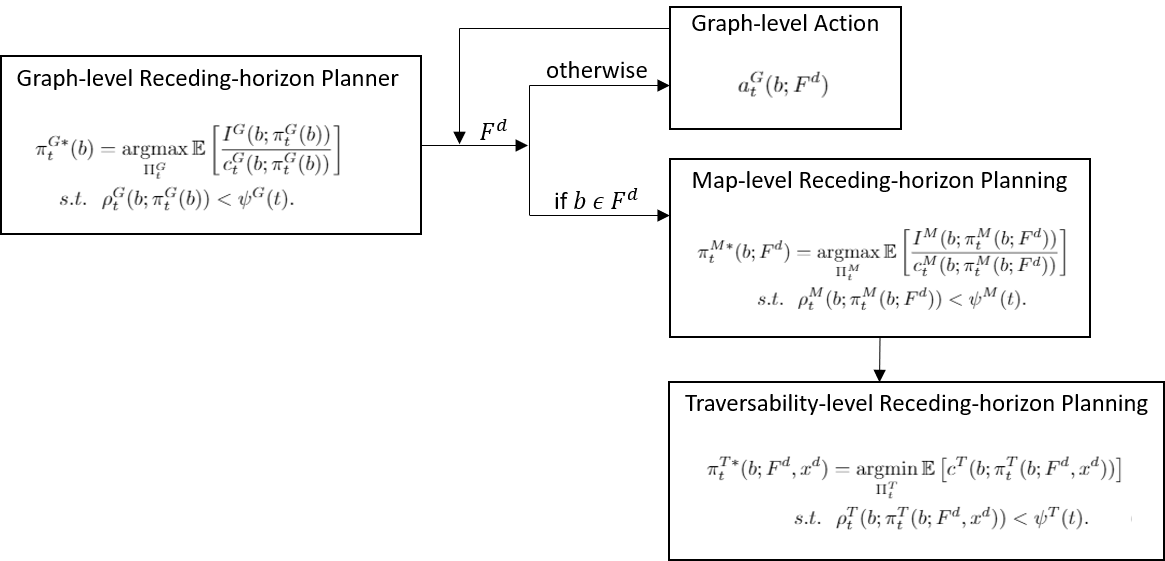
\includegraphics[width=.9\textwidth]{figures/structure.png}
%   \label{fig:architecture}
% \end{figure*}

% \begin{figure*}[ht!]
% %   \centering
%   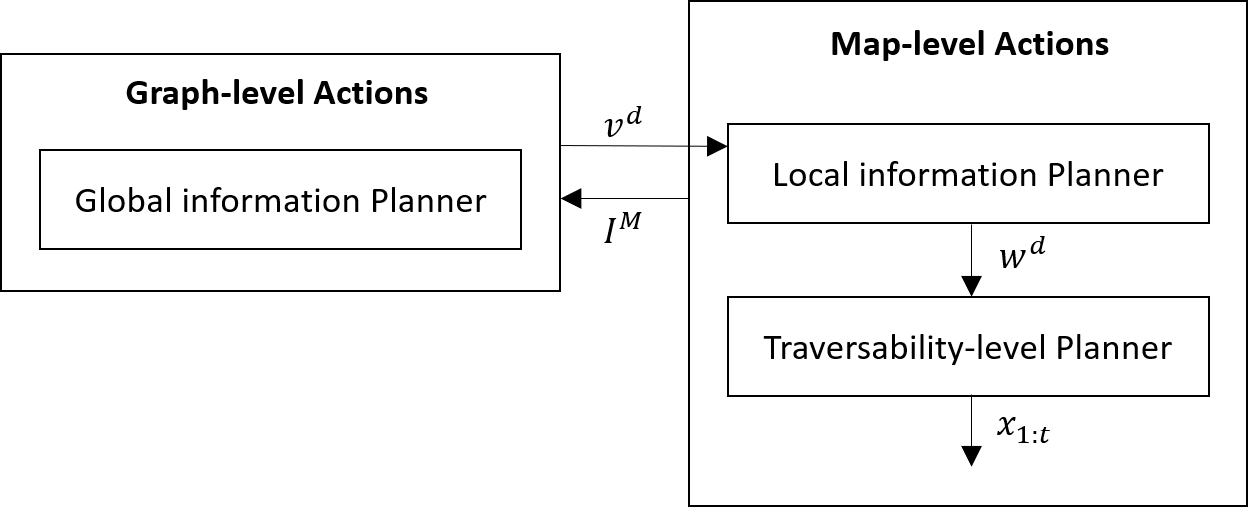
\includegraphics[width=.48\textwidth]{figures/structure_v2.png}
%   \label{fig:architecture}
% \end{figure*}

\ph{Graph Definition}
We employ a sparse graph structure $G = (V, E)$ captures the connectivity of the free space in the environment.  We refer to this graph as the IRM (information roadmap) as its nodes ($V$) and edges ($E$) are enriched by various environmental and robot-related properties.  In general, we consider a graph of sampled beliefs, i.e. where $V=\{v|v\in\mathbb{B}\}$ and edges $E$ are a set of actions and measurements the robot can take to transition between two belief nodes. Constructing a graph which densely samples the full beliefs space suffers from the curse of dimensionality and may be intractable.  Instead, we incrementally sample the belief space \textit{locally}.  We grow the IRM graph as the robot explores, creating new nodes, both leaf nodes and internal nodes.  We distinguish between two types of nodes:  breadcrumb nodes and frontier nodes.  Roughly speaking, breadcrumb nodes $b\in B \subset V$ encode the connectivity of free and traversible space where the robot has explored already, and frontier nodes $f\in F\subset V$ encode additional information about the value of exploring new locations, with $F\cup B = V$ (see Figure \ref{fig:irm_large}).

\ph{Belief graph notation}
For ease of notation we make the following definitions.  For a given node $v_i$ with belief $b_i = p(M,x)$, we say the node is \textit{centered at} a location $x^i\in\mathbb{X}$ when $p(d(x,x^i)>r_x)<\epsilon$, for some distance metric $d(\cdot,\cdot)$, \textit{breadcrumb radius} $r_x>0$, and probability threshold $\epsilon\in(0,1]$.  Similarly, we consider a robot with belief $b_t$ to be \textit{at} a node $v_i$ when $p(d(x,x^i)>r_x)<\epsilon$.  Finally, we assume that the IRM contains the latest belief of the map $M_t$ at each node, i.e. $v_i=p(M_t,x^i),\,\forall t$.  We can therefore use the notation $v_i$ to denote the location the node is centered at $x^i$, since we assume the map belief at each node is the most recent belief.

\begin{figure}[ht!]
  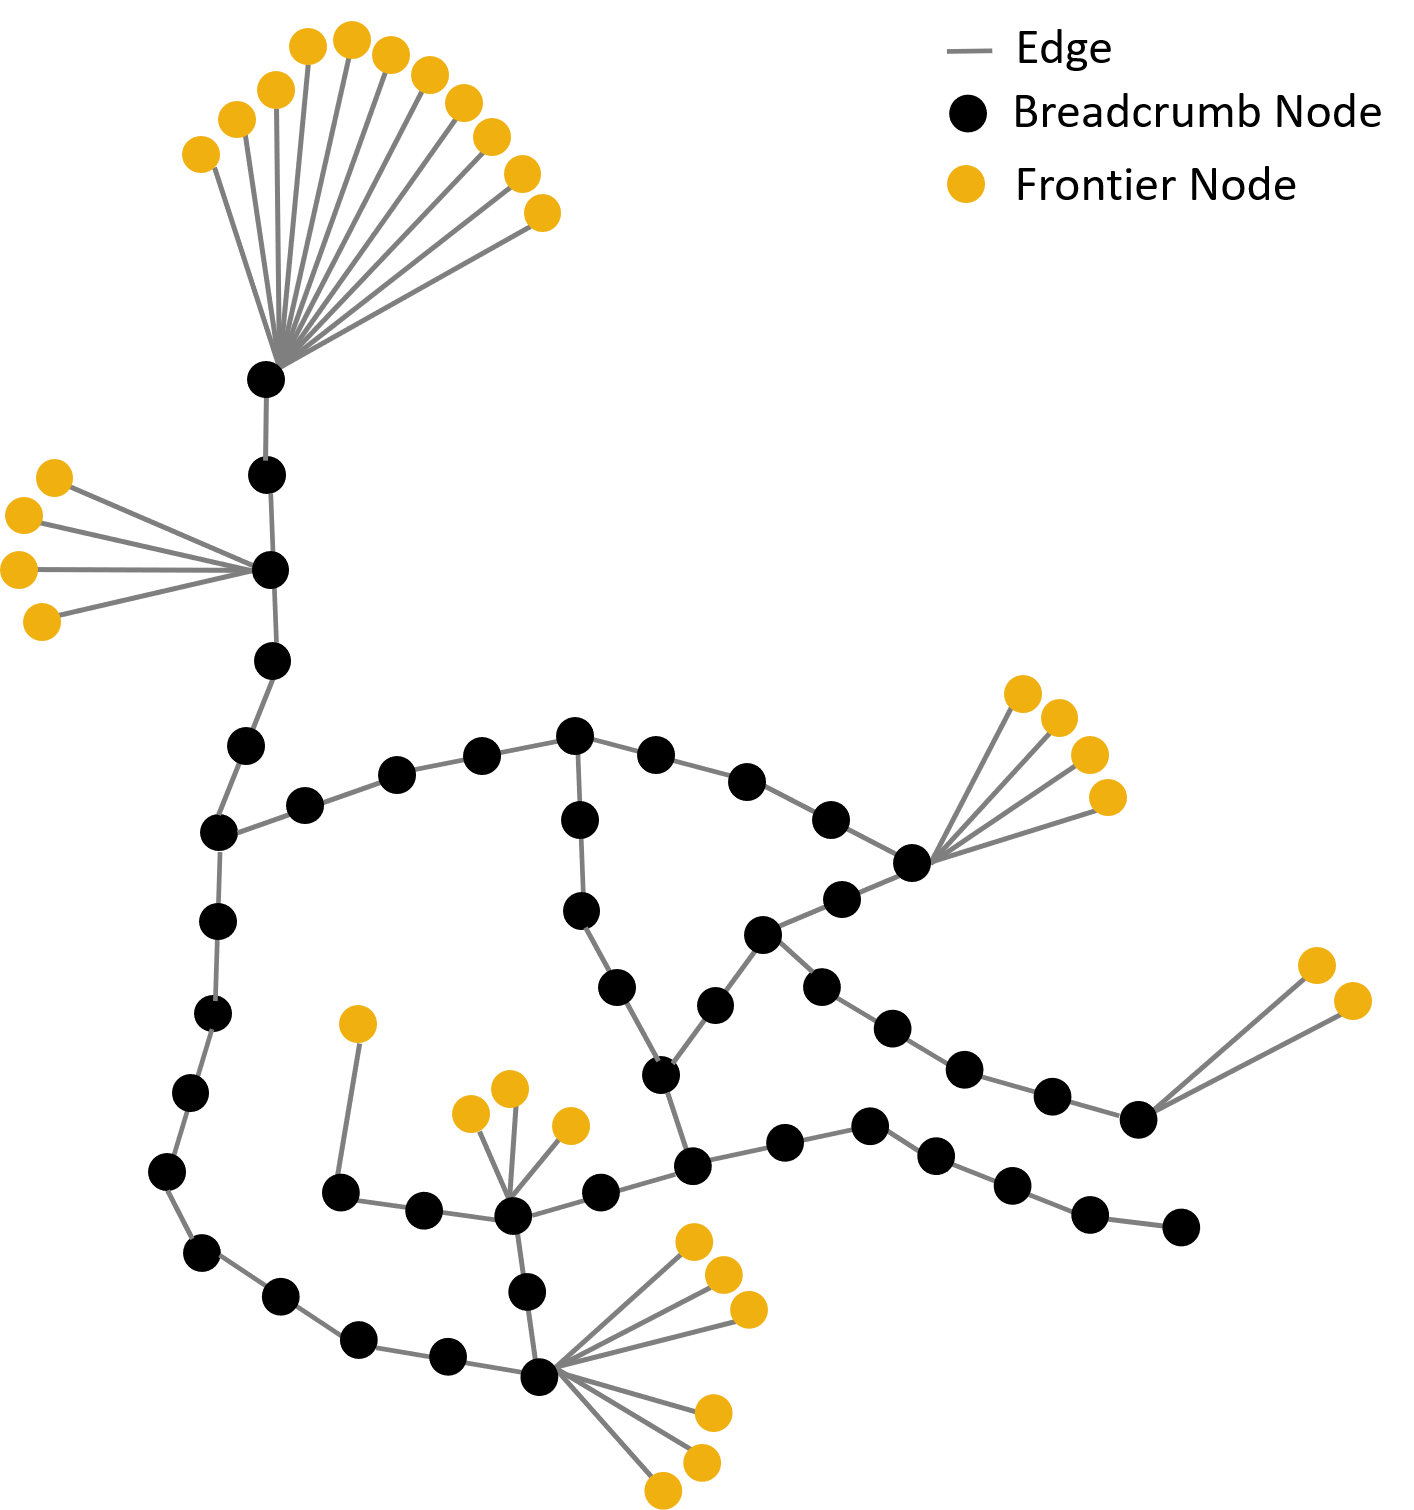
\includegraphics[width=.48\textwidth]{figures/irm.png}
  \caption{Information Roadmap consisting of breadcrumbs and frontiers for belief-space planning over large environments and timescales.}
  \label{fig:irm_large}
\end{figure}

\begin{figure}[ht!]
  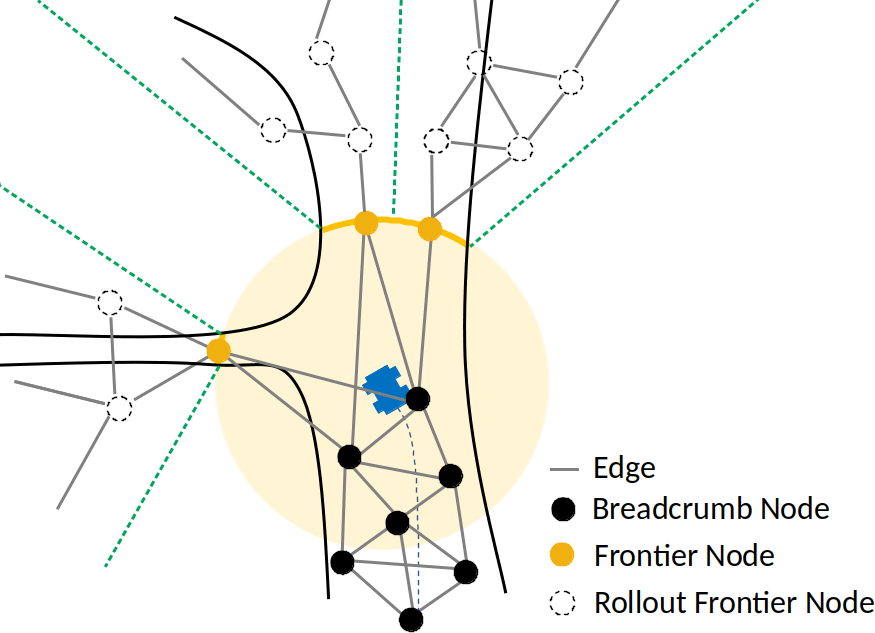
\includegraphics[width=.48\textwidth]{figures/irm_breadcrumbs_frontiers.png}
  \caption{Breadcrumbs (black dots) denote explored regions and help to define to connectivity of free space.  The yellow circle denotes the sensing range.  Yellow dots are new frontier nodes, which encode locations of high potential for information gain.  This potential can be evaluated through rollouts of simulated additional frontier nodes (dotted circles).  In this work we employ an information gain heuristic to approximate these rollouts, as a function of uniquely unexplored territory (area between dashed green lines).}
  \label{fig:breadcrumbs_frontiers}
\end{figure}

\ph{Breadcrumb nodes}
% We refer to leaf nodes as frontiers $f\in F\subset V$ and internal nodes as breadcrumbs $b\in B \subset V$ with $F\cup B = V$.  New internal nodes capture the connectivity of free space to allow for efficient future traversal. 
Breadcrumb nodes $b\in B \subset V$ are nodes centered at locations where \textit{no changes to the map belief will occur}.  This means that we consider breadcrumb nodes to be locations where the map is fully explored.  Note that this does not require the exact location to have been visited before (see Figure \ref{fig:breadcrumbs_frontiers}). 

\ph{Frontier nodes (1-step lookahead)}
We define a frontier node $f\in F\subset V$ as a node centered at a location where we expect to see changes to the map belief.  We can generate these frontiers by applying a look-ahead policy (a rollout).  This rollout simulates how the graph will grow by taking multiple actions into the future, and can be constructed using simulations derived from models of the environment, heuristics, etc.  For the frontier $f$ with planning depths $k$, we can write the belief of the frontier to be $b_{f,k} = p(M_k, x_k = x_f)$.

\ph{Frontiers can encode a k-step lookahead}
In this work, we because we assume that we have limited sensing range in a completely unknown environment, we add frontiers to the graph with a one-step look-ahead only.  By adding frontiers on the boundary of known vs. unknown space, we avoid adding large numbers of spurious nodes which could be located inside obstacles, walls, etc.  However, to account for higher planning depths and avoid myopic behavior, we treat each one-step lookahead frontier as a representative of an entire isolated lookahead  subtree which extends from the frontier, and which excludes the branch coming back to IRM breadcrumb node.  In doing so, we assume the robot may move to a frontier, grow a subtree of new nodes and explore them, then return to the original frontier.  We encode in the frontier the expected change to the belief from exploring the whole subtree as a bonus to the expected information gain, as will be shown later.

% \note{(Sung) I suggest we define `frontier nodes' as `virtual/simulated nodes from one-step look-ahead (rollout)', which would be more coherent to the original meaning. The breadcrumb nodes with connected frontier nodes are the original leaf nodes, but we expand our graph by one-step look-ahead at every leaf node, and we solve for the graph policy on the expanded graph (where the frontier nodes are now the leaf nodes).}
% \hn{Frontier nodes is better, since it keeps the discussion generic. Technically, the current method herein is not 'virtual/simulated nodes from one-step look-ahead (rollout)'... Since your past papers didn't care about ignoring entire processes for 'generative models', why not remove rollout and just call it 'generative model'?}
% \note{(Sung) Actually I meant two things at the same time here, and was not that clear.
% But beforehand, we need to clearly distinguish $v \in V$ and $b = p(M, x) \in \mathbb{B}$, where $x \in V$ on the IRM approximately, in this dicussion as well as in the whole text.
% Now what I meant to say:
% i) Frontier node pose $x_f \in \mathbb{X}$ is generated from one-step look-ahead (from ray casting, a generative model, or whatsoever), and
% ii) a frontier belief node $b_{f,k} = p(M_k, x_k = x_f)$ on the belief tree at planning depth $k$ is a representative of the whole subtree excluding the branch coming back to IRM breadcrumb node.
% It is for the abstraction that can leave our framework generic without opting for a specific approach (heuristic, generative model, deep learning, etc.).
% @Henry: I would like a further discussion about the capability of estimating $J(b_{f,k})$ for given parameters such as a planning depth into the subtree and a flag to return to the original pose $x_f$ at the end of the subtree.}


%We first introduce Information Roadmap (IRM) which is a sparse graph that encodes the connectivity of the free space in the environment and other abstract information such as node-to-node traversability.

%\subsection{Information Roadmap (IRM)}

% \begin{align}
%     u = \pi(b) = \pi^{traversability} (\pi^{EntropyMaximizer} ( \pi^{graph} (b) ) )
% \end{align}

% \begin{align}
%     u = \pi(b) = \pi^{T} (\pi^{M} ( \pi^{G} (b) ) )
% \end{align}
%\todo{Do we want to define multiple edges between nodes?}


% \subsubsection{IRM construction/update}

% \ph{Breadcrumb node generation} Breadcrumbs are generated...

% \ph{Breadcrumb node wiring}

% \ph{IRM update at loop closure}
% Automatic IRM edge updates on loop closure ensures that the IRM topology matches with the underlying pose graph after a loop closure has occurred.

% \begin{figure}[ht!]
%   \includegraphics[width=.48\textwidth]{example-image}
%   \centering
%   \caption{IRM}
%   \label{fig:irm}
% \end{figure}


\ph{Frontier detection and pruning}
The frontier detection/pruning process in our framework serves as an encoder of the mapping information to a graph level.
From the local occupancy grid map, it keeps track of the border of the known free and unknown spaces, so-called \textit{frontiers}, and updates the frontier nodes on the IRM accordingly.
This enables the IRM to effectively capture the information of the coverage of the whole environment, while keeping its simple representation structure.


\ph{Graph policy}
We define the graph-level policy $\pi^g \in \Pi^g$ as a function that returns a controller-specific parameter vector $\theta\in\Theta\subseteq\mathbb{R}^{n_\theta}$ given the current node $v \in V$.
\begin{align}
    \pi^g(v): V\rightarrow \Theta
\end{align}
For example, $\theta$ could represent the location of the next node to reach, specific gains for an LQR controller, weights of a neural network, etc.

\ph{Map policy}
We define the map-level policy $\pi^M \in \Pi^M$ as a function that uses a controller-specific parameter vector $\theta\in\Theta\subseteq\mathbb{R}^{n_\theta}$ given the current belief $b$, and returns a local action.
\begin{align}
    \pi^M(b;\theta): \mathbb{B}\times\Theta\rightarrow \mathbb{A}
    % \pi^M: b(s)\rightarrow a
\end{align}
% \note{$\pi^M(b ; v) = RHC(b; v,m)~~OR~~ LQG(b; v,m)$}

\ph{Overall policy}
We define an overall policy $\pi \in \Pi$ generated by combining the graph-level policy $\pi^g$ and the map-level policy $\pi^M$.
\begin{align}
    \pi(b;v):\mathbb{B}\times V\rightarrow \mathbb{A}
\end{align}
Given the current node, the graph-level policy chooses the next local controller, and the map-level policy generates the corresponding local control signal at belief $b(s)$. This overall policy is stated as follows:
\begin{align}
    \pi(b;v) = \pi^M(b; \pi^g(v))
\end{align}

At the graph-level, we assume that $\pi^M$ is fixed and thus only optimize over $\pi^g$, which implies optimizing at the node-to-node level. However later we will show how we optimize over $\pi^M$ as well.

\subsection{Graph-Level Planning}

\ph{Graph edge transition}
Given a graph-level policy $\pi^{g}(v_i)$, control signals generated by the map-level policy will induce a  transition from nodes $v_i$ to $v_j$ with some probability:
\begin{align}
    T^{g} (v_i, \pi^g(v_i), v_j) = \prod_{t}^{t+\tau} T(x_t,\pi(b_t;v_i),x_{t+1})
\end{align}
where $\tau\in\mathbb{N}$ is the number of timesteps the policy $\pi^M(b;\pi^g(v_i))$ is executed for, and where we assume that $x_{t+\tau}$ is at the goal node $v_j$.  Note that $\tau$ may vary depending on $v_i$ and $\pi(\cdot;v_i)$.

\ph{Graph edge information reward}
We define the graph action information reward $I^g(v, \pi^M): V \times \Pi^M \to \mathbb{R}$ as the amount of information gain when moving from a node $v_i$ under a policy $\pi^M$.
\begin{align}
    I^g(v_i,\pi^M) = \mathbb{E}_{\pi^M(\pi^g(v_i))}\left[\sum_{t}^{t+\tau}  I(b_t,a_t)+\hat{I}^{g}(v_j)\right]
    \label{eq:graph_action_info_reward}
\end{align}

where $\hat{I}^{g}(v_j)$ is the graph expansion reward, defined as follows:

\ph{Graph expansion reward for frontier nodes}
The graph expansion information reward associated with a frontier node $v_j \in F$ encodes the value of expanding the IRM by the addition of frontier child nodes. We denote the expected value of a frontier node by $\hat{I}^{g}(v_j)$.

There are several ways to compute $\hat{I}^{g}(v_j)$, $\forall v_j \in F$:
i) based on the collected information so far (e.g., the frontier cell segment size),
ii) based on the domain knowledge or heuristic estimation, or
iii) via Monte Carlo simulations (i.e., rollouts) beyond the leaf nodes based on the prior or learned models.
Note that for unknown complex environments, it is hard to construct reliable prior or learned models for the third approach.

\ph{Graph edge reward}
We define the graph reward as the reward gained by executing the graph-level policy $\pi^g$ from node $v$ as a function $R^g(v, \pi^g): V \times \Pi^g \to \mathbb{R}$.  For example, the reward could be a function of information gain, risk, or time of travel:
\begin{multline}
    R^g(v, \pi^g(v)) = f(I^g(v,\pi^M(\pi^g(v))),\\
    \rho(v,\pi^M(\cdot,\pi^g(v))),\tau(v,\pi^M(\cdot,\pi^g(v)))
\end{multline}
where $\rho$ and $\tau$ are possible functions to encode information about risk and time taken along the trajectory, and $f$ combines the information to produce a reward value.

\ph{Planning horizon on the graph}
Recall the total time horizon for the problem in Eq. (\ref{eq:artifactopt_cost}) is $L$.  We wish to discretize this into $K$ larger chunks of time on the graph.  For example, if we assume a fixed time to traverse between any two nodes of $\tau$, then $K$ can be the number of transitions to optimize over on the graph: $K=ceil(L/\tau)$.  When $\tau$ varies depending on the node and policy, then we may approximate $K$ with some heuristic.

\ph{Time-varying graph policy}
Up to this point we have omitted the time dependence of the policy $\pi^g(v)$ from the notation, however because we wish to solve a finite horizon problem, the policy needs to be time-varying.  With a slight abuse of notation, let $k=0,\cdots,K$ indicate the graph-level timesteps, and we write our time-varying graph policy as $\pi^g_k(v)$. 

\ph{Graph value function}
Next we define the graph value function $J^g(v,k;\pi^g_{k:K})$ as the sum of future expected rewards on the graph for a graph-level policy $\pi^g$ as:
\begin{align}
    % U^g(b) = f(I^E, c(b, \pi^g)) \\
    J^g(v_i,k;\pi^g_{k:K}) &= \mathbb{E}_{\nu_{k'}\sim T^g,\, \nu_k=v_i} \left[ \sum_{k'=k}^K R^g(\nu_{k'}, \pi^g_{k'}(\nu_{k'})) \right]
    \label{eq:graphvaluefn}
\end{align}

\ph{Graph-level optimization problem}
We wish to find the optimal graph level policy $\pi^g_{k:K}$ over timesteps $k$ to $K$ in a receding horizon manner that maximizes the value function over the space of possible policies $\Pi^g_{k:K}$:
\begin{equation}
    \pi^{g*}_{k:K}(v)=\max_{\Pi^g_{k:K}} J^g(v,k;\pi^g_{k:K}).
    \label{eq:graphoptprob}
\end{equation}


% \begin{equation}
%     J^{g*}(v_i,\pi^g_{i:\infty})=\max_{\Pi^g_{i:\infty}} J^g(v_i;\pi^g(v_i)).
%     \label{eq:graphoptprob}
% \end{equation}

% The Bellman equation is used to find the optimal graph-level policy $\pi^g$ that maximizes the value function over the space of possible policies $\Pi^g$:
% \begin{align}
% \pi^{g*}(v_i)
%     &= \argmax_{\Pi_{0:\infty}^g} \Big[R^g(v_i, \pi^g(v_i)) \nonumber \\
%     &\quad\quad + \sum_{v_j \in V} T^g(v_i, \pi^g(v_i),v_j) J^{g*}(v_j) \Big]
%     %\\ &s.t.~~J^{g*}(v_j) = \hat{J}^{g*}(v_j),~~\forall~ v_j \in F \nonumber
%   \label{eq:bellman_opt_approx}
% \end{align}

% \noindent where $\hat{J}^{g}(v_j)$ is the expected graph value for frontier nodes, as detailed below. 


\ph{Graph planner - belief tree search}
Now we describe how we can solve Eq.~(\ref{eq:graphoptprob}).
Since $J^g(v_i,k; \pi^g)$ depends on the \textit{sequence} of actions as defined in Eq.~(\ref{eq:graphvaluefn}), we cannot use a simple value iteration on the IRM (as in the MDP setting), which accepts the Bellman update in any arbitrary order.
Instead, we need to construct a tree structure, called a \textit{belief tree}, rooted at the current given node $v_i$ at timestep $k$, and growing until reaching a leaf node or the finite horizon.
% \note{When thinking of probabilistic occupancy state estimation (i.e., we may not get rid of occupancy state uncertainty by a single visit), then we may end up having an infinite-horizon belief tree. So, we should not say we can solve for infinite horizons even with i) or ii) scheme.}
%
This tree structure will unroll the graph with possible loops, and encodes the dependency on the history
(e.g., revisiting a leaf node multiple times will not provide a multiple of the leaf node's original information gain).

% \begin{figure}[ht!]
%   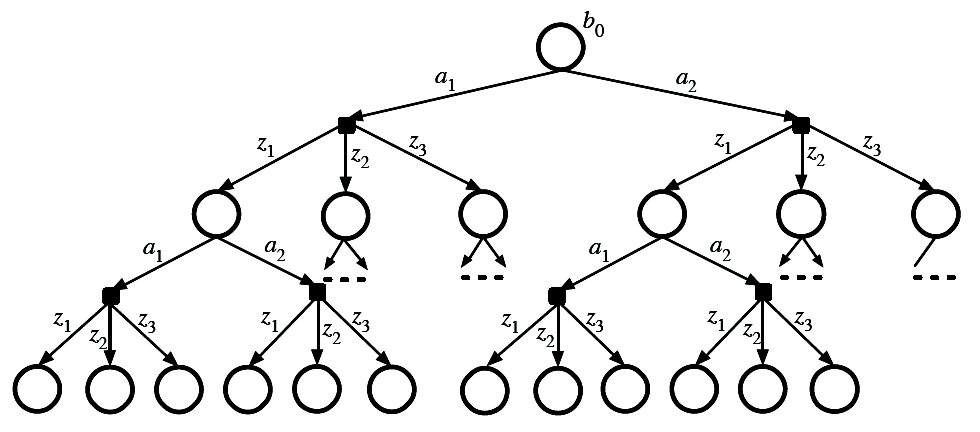
\includegraphics[width=.48\textwidth]{figures/search_tree.png}
%   \caption{Because the expected information gain will change after taking an action, we must construct a decision tree with time dependencies.}
%   \label{fig:search_tree}
% \end{figure}

\ph{Algorithm description}
In order to solve Eq.~(\ref{eq:graphoptprob}), we need a belief tree search algorithm.
At a high level, we need to i) construct a belief tree that contains all the reachable nodes from the root node, and ii) update the expected value for each node by value backpropagation from the leaf nodes.
iii) Once the expected value for each action for each node converges after enough iterations of i) and ii), we return the best action for each node that maximizes the expected value.
% \todo{We can add a pseudo-code algorithm.\!\!}


\begin{figure}[ht!]
  \centering
  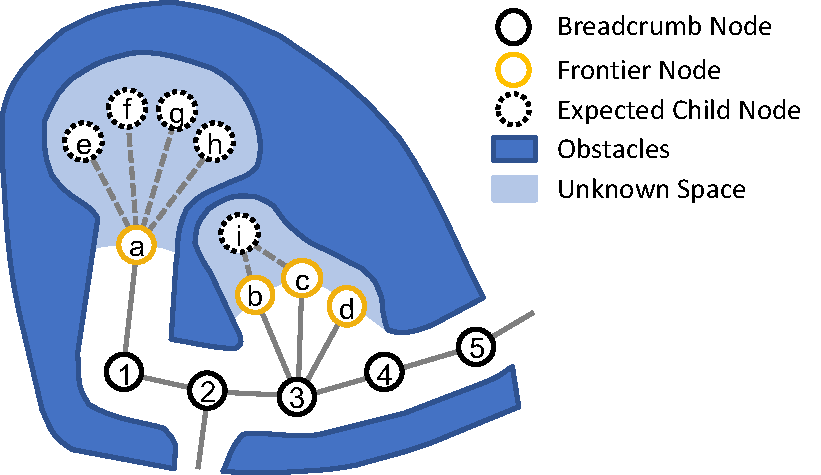
\includegraphics[width=.8\columnwidth]{figures/bts_example/bts_irm.pdf}
  \caption{Toy example: IRM}
  \label{fig:bts_irm}
\end{figure}
\begin{figure}[ht!]
  \centering
  \subfloat[$M_{0}$]{%
    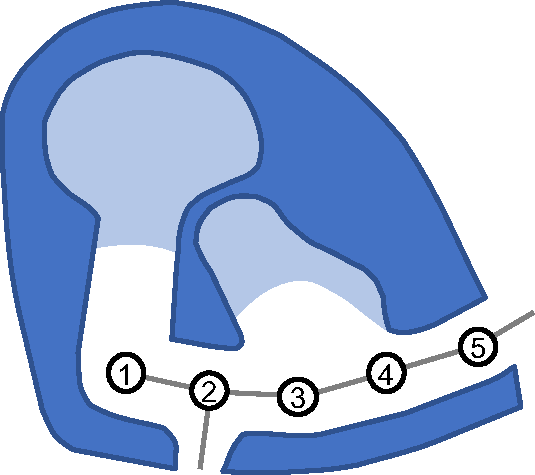
\includegraphics[width=0.3\columnwidth]{figures/bts_example/bts_map0.pdf}
  }
  \subfloat[$M_{01}$]{%
    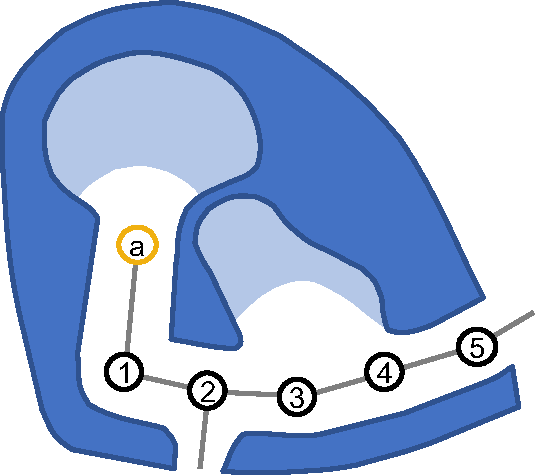
\includegraphics[width=0.3\columnwidth]{figures/bts_example/bts_map01.pdf}
  }
  \subfloat[$M_{1}$]{%
    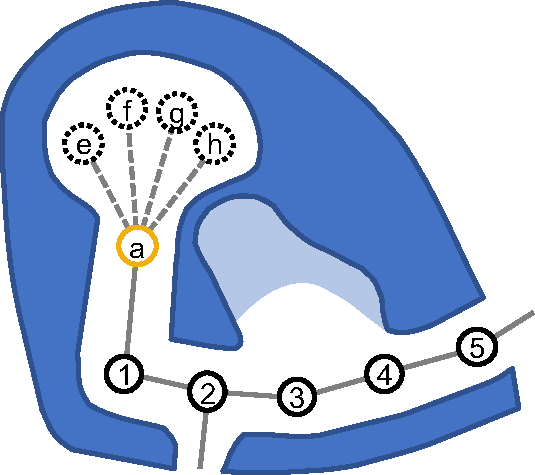
\includegraphics[width=0.3\columnwidth]{figures/bts_example/bts_map1.pdf}
  }
  \\ 
  \subfloat[$M_{02}$]{%
    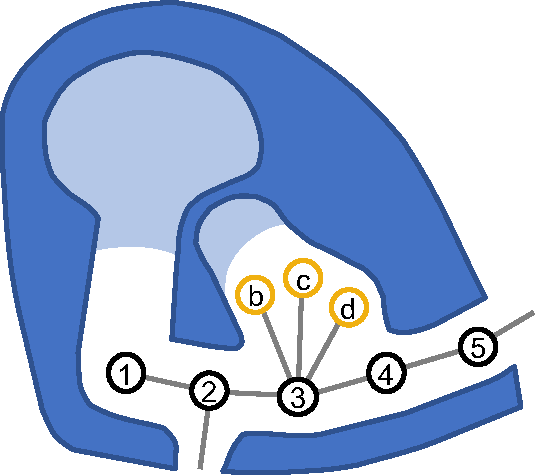
\includegraphics[width=0.3\columnwidth]{figures/bts_example/bts_map02.pdf}
  }
  \subfloat[$M_{2}$]{%
    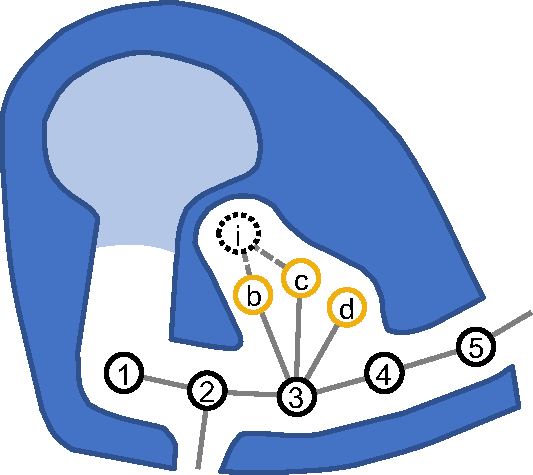
\includegraphics[width=0.3\columnwidth]{figures/bts_example/bts_map2.pdf}
  }
  \subfloat[$M_{3}$]{%
    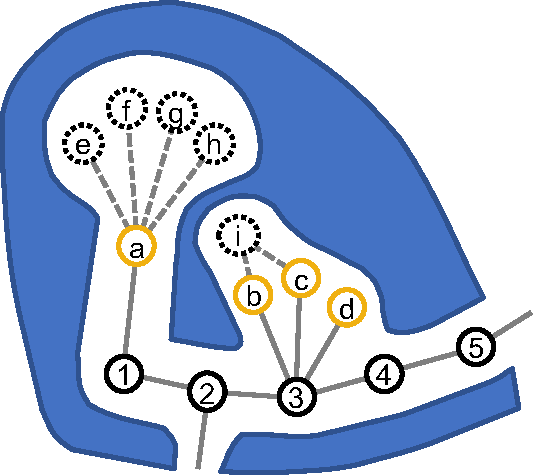
\includegraphics[width=0.3\columnwidth]{figures/bts_example/bts_map3.pdf}
  }
  \caption{Toy example: Map beliefs depending on history.}
  \label{fig:bts_maps}
\end{figure}
\begin{figure}[ht!]
  \centering
  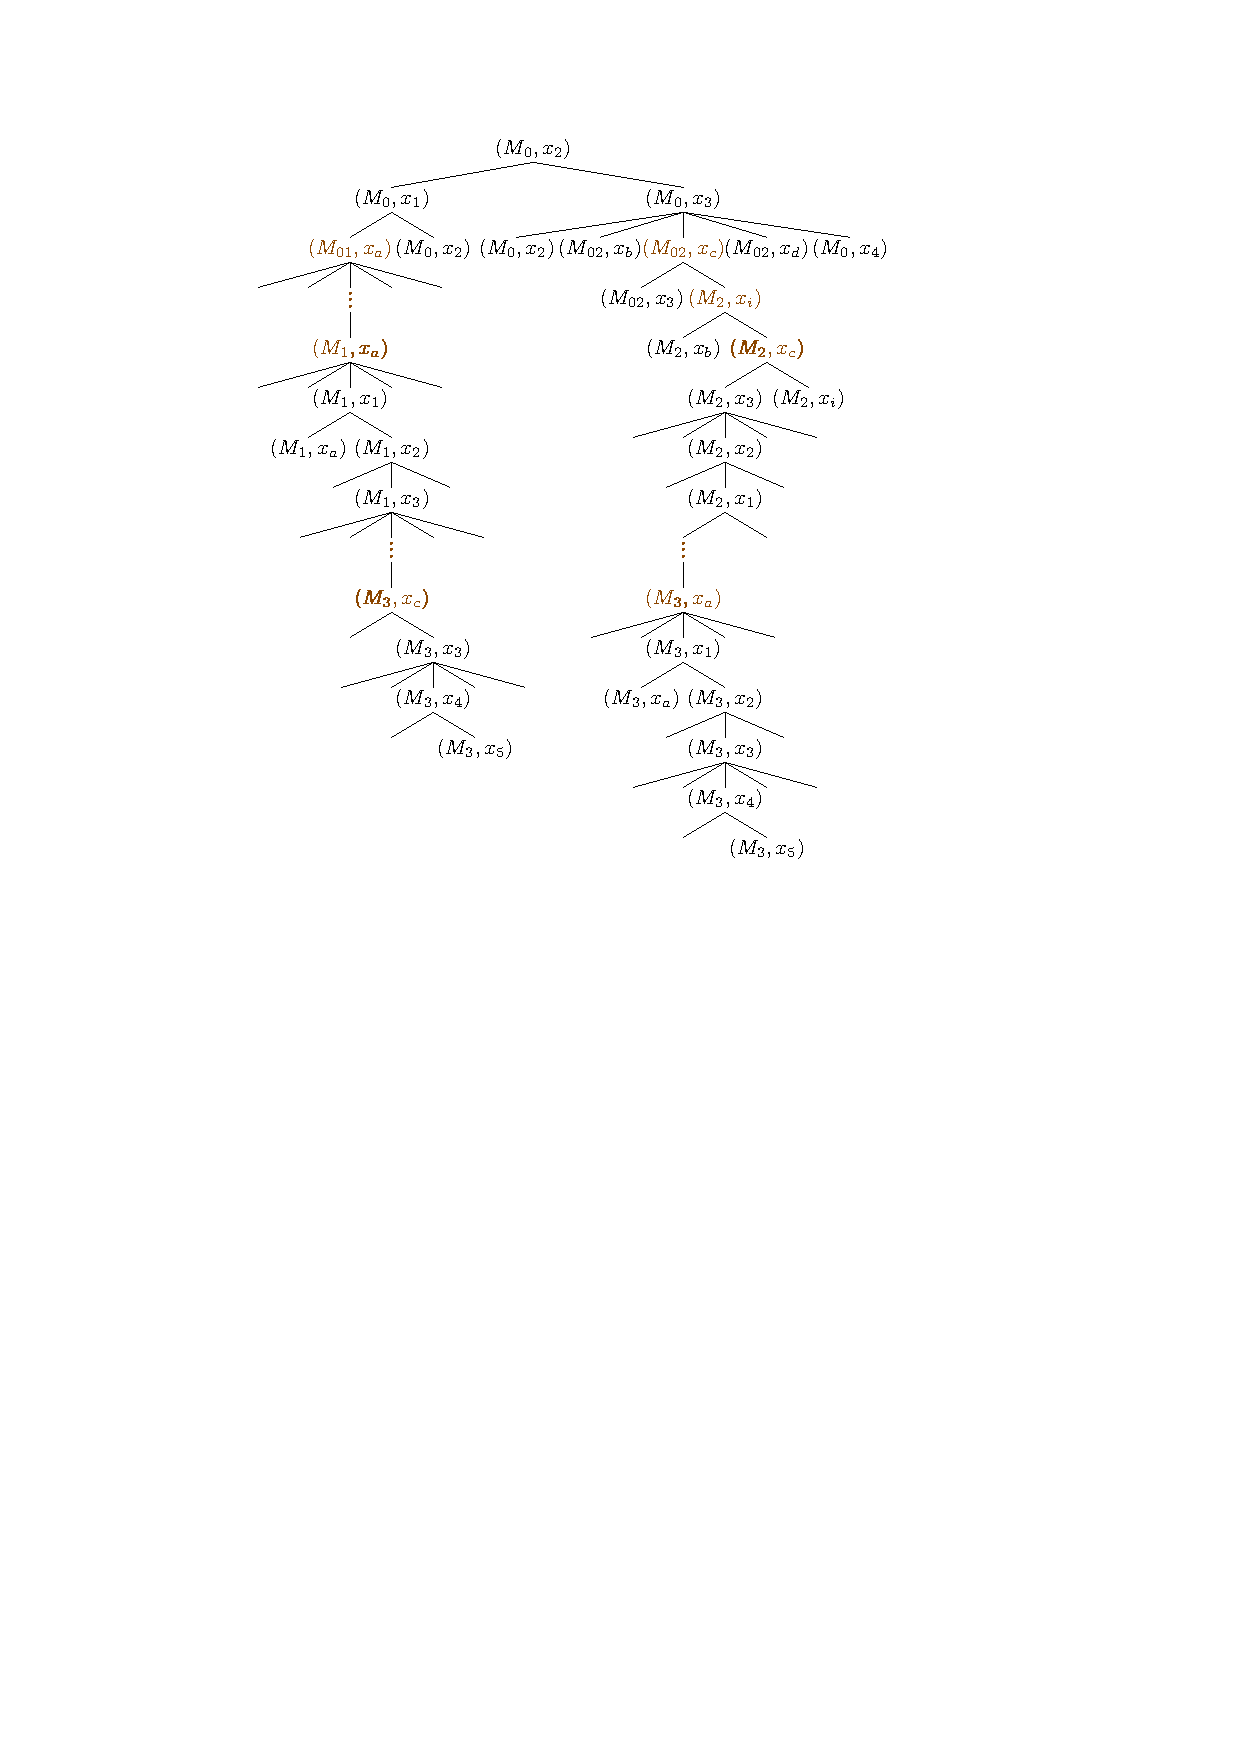
\includegraphics[width=\columnwidth]{figures/bts_example/bts_example.pdf}
  \caption{Toy example: Belief tree search}
  \label{fig:bts_example}
\end{figure}

\ph{Toy example}
We describe the belief tree search process for a simple toy example.
Herein, let us consider the maximum likelihood state as a belief state and assume the observations to be deterministic.
The current IRM is as shown in Figure~\ref{fig:bts_irm}, and the robot is expected to be at the breadcrumb node 2, i.e., $x_2 \in \mathbb{X}$, with the latest map estimation $M_0$ in Figure~\ref{fig:bts_maps}.

Taking the current belief $b_0 = (M_0, x_2)$ as the root node, we can construct a belief tree as shown in Figure~\ref{fig:bts_example}.
From the root node, there are two possible actions; moving to $x_1$ or $x_3$, while both of them will not be able to reduce the map uncertainty.
In the case the robot moves from $x_3$ to $x_c$ and to $x_i$, a part of the map is uncovered, and the map belief is updated from $M_0$ to $M_{1}$.
On the way back to $x_3$, the map belief will not change.

Once a belief tree along the possible actions and updated beliefs is constructed up to a finite horizon, we can compute the graph value function for each node by backpropagating the value of the leaf node and the graph edge rewards along the branch.
In this example, we can decide to move to $x_1$ from the current state since it can provide the same amount of information gain for a smaller action cost.


\ph{Remark} We can improve the efficiency of this process in various ways \cite{silver2010monte,somani2013despot,bonet1998learning,kim2019pomhdp}.
For example, we interleave the belief tree construction and belief tree search, so that we first focus on the subset of the tree that is likely to be included in the optimal policy tree. As for the planning horizon, we can use a fixed (discounted) horizon if $K$ is too large, but it can be useful to incorporate a variable finite horizon that can scale over different sizes and structures of the IRM.

% \ph{Graph planner}

% \begin{itemize}
% \item \ph{Expected value for open-ended leaf nodes}
% % \item \ph{Graph expansion information reward}
% With incomplete exploration of the environment, the IRM is also incomplete---there are open-ended leaf nodes (i.e., frontier nodes) whose successor nodes are expected to exist but not yet created. \todo{Needs better wording here.\!\!}
% We denote the expected value of an open-ended leaf node $v_j \in F$ by $\hat{J}^{g}(v_j)$.

% There are several ways to compute $\hat{J}^{g}(v_j)$, $\forall v_j \in F$;
% i) based on the collected information so far (e.g., the frontier cell segment size),
% ii) based on the domain knowledge or heuristic estimation, or
% iii) via Monte Carlo simulations (i.e., rollouts) beyond the leaf nodes based on the prior or learned models.
% Note that for unknown complex environments, it is hard to construct reliable prior or learned models for the third approach.

% % We notate the expected value of an open-ended leaf node $v_j$ as:
% % \begin{align}
% %     % I^G(v_i,v_j) = \sum_{s\in e_{ij}} I(s,\pi^M(s)) \\
% %     I^V(v_j) = I^{future}(v_j)
% % \end{align}
% % where $I^{future}(v_j)$ is the expected future information gain which results from the ability to add new nodes to the graph after executing a policy $\pi^g(v_j)$.

% \item \ph{Belief tree search algorithm}

% \emph{Reason for belief tree search:}
% Now we describe how we can solve Eq.~(\ref{eq:graphoptprob}).
% Since $J^g(v_i, \pi^g)$ depends on the \textit{sequence} of actions as defined in Eq.~(\ref{eq:graphvaluefn}), we cannot use a simple value iteration on the IRM (as in the MDP setting), which allows the Bellman update in any arbitrary order.
% Instead, we need to construct a tree structure, called a \textit{belief tree}, rooted at the current given node $v_i$ at $k=0$, and growing until reaching a leaf node or the finite horizon.
% % \note{When thinking of probabilistic occupancy state estimation (i.e., we may not get rid of occupancy state uncertainty by a single visit), then we may end up having an infinite-horizon belief tree. So, we should not say we can solve for infinite horizons even with i) or ii) scheme.}
% %
% This tree structure will unroll the graph with possible loops, and encodes the dependency on the history
% (e.g., revisiting a leaf node multiple times will not provide a multiple of the leaf node's original information gain).

% \emph{Algorithm description:}
% In order to solve Eq.~(\ref{eq:graphoptprob}), we need a belief tree search algorithm.
% Basically, we need to i) construct a belief tree that contains all the reachable nodes from the root node, and ii) update the expected value for each node by value backpropagation from the leaf nodes.
% \todo{We can add a pseudo-code algorithm.\!\!}

% We can improve the efficiency of this process in various ways \cite{silver2010monte,somani2013despot,kurniawati-isrr13}.
% For example, we interleave the belief tree construction and belief tree search, so that we first focus on the subset of the tree that is likely to be included in the optimal policy tree.

% As for the planning horizon, we can use a fixed (discounted) horizon, but it can be useful to incorporate a variable finite horizon that can scale over different sizes and structures of the IRM.

% \end{itemize}

% At each step, we can solve the simple one-step optimization via the Bellman equation:
% \begin{align}
% \pi^{G*}(v_i)
%     &= \argmax_{\Pi_{0:\infty}^g} \Big[U^g(v_i, \pi^G(v_i)) \nonumber \\
%     &\quad\quad + \sum_{v_j \in V} T^g(v_i, \pi^G(v_i),v_j) J^{g*}(v_j) \Big] \\
%     &s.t.~~J^{g*}(v_j) = I^V(v_j),~~\forall~ v_j \in F
%   \label{eq:bellman_opt_approx}
% \end{align}

% Every frontier is an attractor, and serves as the root of a tree. Given that there's multiple frontiers in a graph, the IRM is a forest that changes with every iteration....


% \ph{Computational tractability}
% Because we have a finite graph with sparse connectivity, finding an optimal cost-to-go $J^{G*}(v_j)$ is much easier than maximizing Eq. (\ref{eq:artifactopt_cost}) and can be efficiently computed via Breadth First Search.


% \todo{
% \begin{enumerate}
%     \item need some node cost or cost of traversal?  time to travel?
% \end{enumerate}
% }

% New frontier nodes capture the boundary between explored and unexplored regions and allow for efficient exploration action selection.

%%%%%%%%%%%%%%%%%%%%%%%%%%%%
% \subsection{Unorganized Stuff for now}

% \begin{align}
%   \pi_{0:T}^*(b)
%   & = \argmax_{\Pi_{0:T}} \mathbb{E} \left[ \sum_{t=0}^T I^M(b_t; \pi_t(b_t)) \right]
%   \label{eq:globalopt}
%   \\
%   & \approx \sum_{t=0}^T \argmax_{\Pi_{t}} \mathbb{E} \left[ \frac{I^M(b_t; \pi_t(b_t))}{c_t^M(b_t; \pi_t(b_t))} \Delta t \right]
%   \label{eq:recedinghorizon}
%   \\
%   & \approx \sum_{t=0}^T \pi_b^{G*}(b) \Delta t.
%   \label{eq:hierarchical}
% \end{align}
% Note that we approximated Eq.~(\ref{eq:globalopt}) to Eq.~(\ref{eq:recedinghorizon}) based on receding horizon planning scheme, and Eq.~(\ref{eq:recedinghorizon}) to Eq.~(\ref{eq:hierarchical}) based on hierarchical optimization scheme.

\subsection{Map-Level Planning}
In this section, we propose a local planner that gathers local map information and takes the traversability information into account. The local planner interacts with the graph planner to maintain the global sense of the information and decision making.  Recall that our graph planner $\pi^g(v_i)$ produces a controller specific parameter vector $\theta$, which encodes information for reaching nearby nodes.  Here we show how to find the map-level policy $\pi^M(b;\theta)$ given $\theta$.

\ph{Action reward}
We define the action reward as the reward gained by executing the map-level policy $\pi^M$ at each timestep as a function $R^M(b_t, \pi^M(b_t;\theta)): \mathbb{B} \times \mathbb{A} \to \mathbb{R}$.  
% $R^M(b_t, \pi^M(b_t;\theta)): \mathbb{B} \times \mathbb{A} \to \mathbb{R}$
% $R^M(b_t, \pi^M(\cdot)): \mathbb{B} \times \Pi^M \to \mathbb{R}$
Similar to the graph reward, the action reward can be a function of information gain, risk, or distances:
\begin{align}
    R^M(b_t, \pi^M(b_t;\theta)) = \hat{f}(I(b_t,\pi^M),\rho(b_t,\pi^M),d(b_t,\pi^M,\theta))
\end{align}
where $\rho$ encodes information about risk and $d(\cdot)$ may encode distance traveled, distance from the goal node, etc.

\ph{Map-level value function}
We define the map-level value function $J^M(b_t, \pi^M): \mathbb{B} \times \Pi^M \to \mathbb{R}$ as the sum of future expected rewards for a trajectory with $\tau$ timesteps as:
\begin{align}
  J^M(b_t,\pi^M(b_t;\theta)) &= \mathbb{E} \left[ \sum_{t'=t}^{t+\tau} R^M(b_{t'},\pi^M(b_{t'};\theta))\right], \label{eq:localplan_cost}
\end{align}

\ph{Map Policy}
We optimize the value function above to determine the best map-level policy.  The problem can be formulated as:
\begin{align}
  \pi^{M*}(b_t;\theta) &= \argmax_{\pi^M(\cdot,\theta)} J^M(b_t;\pi^M(\cdot,\theta))
  \nonumber \\
  s.t.~&~\rho(b_t,\pi^M(\cdot,\theta)) < \psi(k)
  \label{eq:mapopt}
\end{align}
where $\rho(b_t,\pi^M(\cdot,\theta))$ is the risk of the trajectory traversing from $b_t$ under policy $\pi^M(\cdot,\theta)$ and $\psi(t)$ is a time-varying acceptable risk threshold.  As the duration of the mission progresses, the risk threshold $\psi(k)$ can increase to allow for riskier actions.


% \section{Bridge section (abstraction of simplifications)}
% \todo{move next section hacks here, but pull out some more general idea of why we do these hacks.}

%%%%%%%%%%%%%%%%%%%%%%%%%%%%%%%%%%%%%%%%%%%%%%%%%%%%%%%%%%%%%%%%%%%%%%%%%%%%%%%%
\section{Algorithmic Assumptions} \label{sec:hierarchical}

In this section, we present implementation details about the hierarchical information-based planner for autonomous exploration in large unknown environments.

\subsection{Grid Representation}
We first describe how we specifically determine information gain in the context of occupancy grid mapping.  In this work, we assume that the artifact object detection works perfectly, and decouple perception from our optimization framework.
In other words, we assume all artifact objects will be detected if the occupancy grid map has been fully covered.

\subsubsection{Occupancy Grid Mapping}
We assume that $\textbf{m}_i$ is associated with a binary occupancy value indicating whether cell is occupied or free.  We restrict the underlying map state space to $\mathbb{M}=\{occupied, free\}$. Calculating the posterior for every single map is intractable, therefore, the problem can be formulated as the posterior over a single grid cell: 
\begin{align}
    p(\textbf{m}_i | z_{1:t},x_{1:t})
\end{align}
Here, we are estimating a fixed, binary state that does not change over time. The posterior is only a function of measurements when a state is time-invariant:
\begin{align}
    p(\textbf{m}_i | z_{1:t},x_{1:t}) = p(\textbf{m}_i | z_{1:t})
    \label{static}
\end{align}
We update the occupancy grid by the Log-Odds method. The \emph{odds} of a state $\textbf{m}_i$ is defined as the ratio of the probability that the cell is free to the probability that the cell is occupied:
\begin{align}
    \frac{p(\textbf{m}_i | z_{1:t},x_{1:t})}{1-p(\textbf{m}_i | z_{1:t},x_{1:t})}
    \label{odd}
\end{align}
The \emph{log-odds} is the logarithm of this ratio:

\begin{align}
    l_{t,i} = \log\frac{p(\textbf{m}_i | z_{1:t},x_{1:t})}{1-p(\textbf{m}_i | z_{1:t},x_{1:t})}
    \label{log_odd}
\end{align}
We can rearrange the \emph{log-odds} ratio to expose the posterior over the grid cell:
\begin{align}
    p(\textbf{m}_i | z_{1:t},x_{1:t}) = 1-\frac{1}{1+\exp(l(\textbf{m}_i))}
\end{align}
Using Bayes filtering, the \emph{log-odds} ratio can be recursively computed using the following expression: 
% \begin{align}
%     l_{t,i} &= \log\frac{p(\textbf{m}_i | z_{1:t-1}, x_{1:t-1})}{1-p(\textbf{m}_i | z_{1:t-1}, x_{1:t-1})} + \log\frac{p(\textbf{m}_i | z_{t},x_{t})}{1-p(\textbf{m}_i | z_{t},x_{t})} \nonumber \\
%     &\quad - \log\frac{p(\textbf{m}_i)}{1-p(\textbf{m}_i)} \nonumber \\
%     &= l_{t-1,i} + \log\frac{p(\textbf{m}_i | z_{t},x_{t})}{1-p(\textbf{m}_i | z_{t},x_{t})} - l_{0,i}
% \end{align}
\begin{align}
    l_{t,i} = l_{t-1,i} + \log\frac{p(\textbf{m}_i | z_{t},x_{t})}{1-p(\textbf{m}_i | z_{t},x_{t})} - l_{0,i}
\end{align}
\noindent where $l_{t-1,i}$ is the previous log-odds value, $l_{0,i}$ is the log-odds representation of the occupancy prior $p(\textbf{m}_i)$, and $p(\textbf{m}_i | z_{t},x_{t})$ is the inverse sensor model.

There are drawbacks of the Log-Odds method, namely the formulation does not reflect dependencies among neighboring cells, and only a single number is stored per cell.  While in the past we have examined mapping algorithms for richer settings \cite{agha2019confidence}, for simplicity we restrain ourselves to the binary occupancy setting in this work.

\subsubsection{Information Gain}
Entropy is a measure for the uncertainty of a posterior. The entropy $H_p(x)$ of a probability distribution $p$ is the expected information $E[-\log p]$. The entropy of the occupancy grid map posterior is
\begin{align}
    H_p(\textbf{m}_i) = -p(\textbf{m}_i) \log p(\textbf{m}_i) - (1-p(\textbf{m}_i)) \log(1-p(\textbf{m}_i))
\end{align}
\noindent and the expected entropy after measuring is $E[H_{p}(\textbf{m}_i)]$. Then the expected information gain when sensing a grid cell $\textbf{m}_i$ is: 
\begin{align}
    I_i = H_p(\textbf{m}_i) - E[H_{p}(\textbf{m}_i)]
\end{align}


\subsection{Frontier detection and pruning}

\begin{figure}[t!]
  \centering
  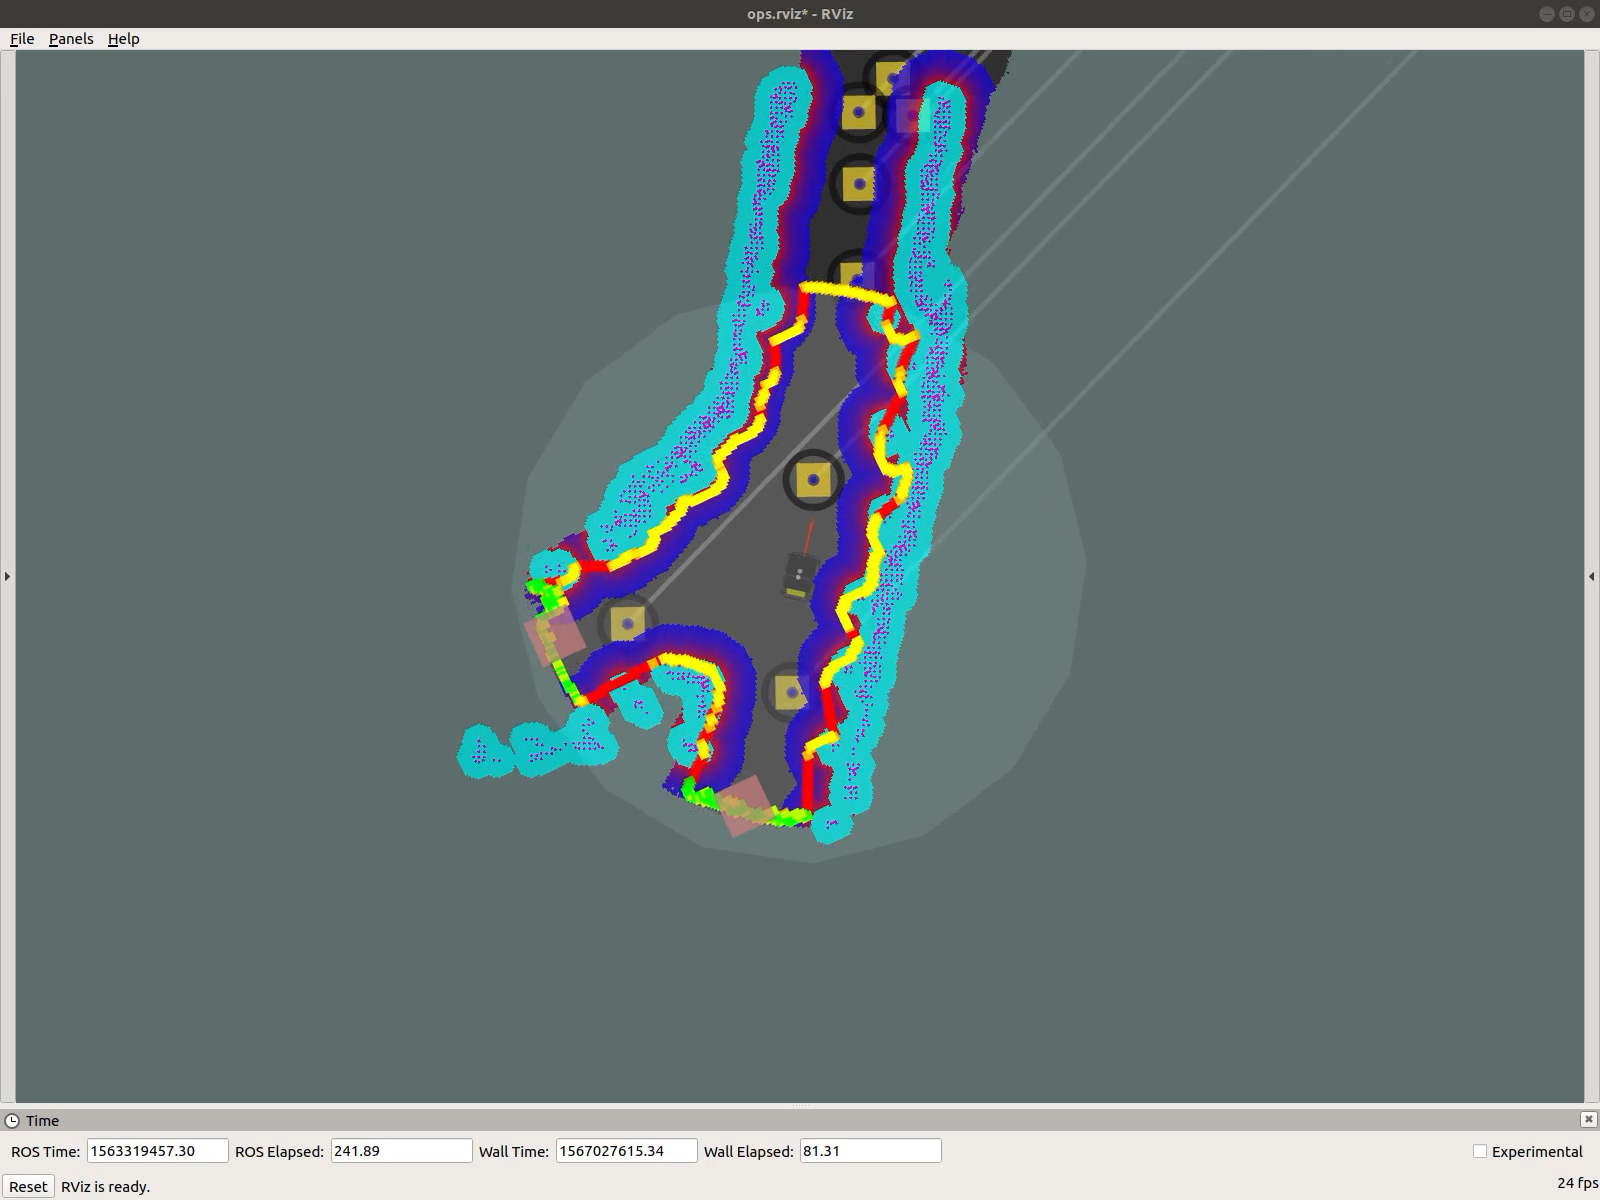
\includegraphics[trim={7cm 9cm 10cm 5cm},clip,width=.48\textwidth,angle=180]{figures/frontier_detection.png}
  \caption{Illustration of frontier detection process.
    From sensor ray end-points (yellow), we extract sensor contour (yellow, red, and green), and detect frontier cells (green) that are adjacent to unknown cells. Then, we sample frontier nodes (pink squares) from the frontier cells.}
  \label{fig:frontiering}
\end{figure}

The frontier detection/pruning process takes an input from the recent range sensor readings and returns a set of frontier nodes to be added or deleted on the IRM.

Frontier detection is composed of several steps, frontier cell detection, frontier node sampling and filtering, and registration to the IRM.

\ph{Frontier cell detection}
Frontier cell detection is based on Fast Frontier Detection algorithm \cite{keidar2012robot} (see Figure~\ref{fig:frontiering}).
From sensor ray end-points (yellow), we extract sensor contour (yellow, red, and green) that connect all the end-points in a sequential order.
Then we detect frontier cells (green) that are adjacent to unknown cells.

\ph{Frontier node sampling}
A frontier node sampled from the detected frontier cells (pink square) as an approximation of the frontier cells.
We determine the frontier node position by computing the centroid of the frontier cells.
If the centroid is not in the known free space, we project it to the nearest frontier cell as an alternative. 

\ph{Frontier node filtering}
In order to prevent having duplicate frontier nodes on the IRM, we filter out new frontiers if they are closer to existing frontier nodes than a threshold.
Additionally, we exclude new frontier nodes if they are near to the pose graph nodes that are generated by other robots.
This is to ensure that new frontiers are not generated where any other robots have explored already.

\ph{Registration of frontier nodes}
Finally, we add the new frontiers to the IRM.
They are connected to the breadcrumb that is closest to the current robot position to encode the visibility for the frontier nodes on the IRM.
We save the relative position to the underlying pose graph node, so that we can keep the same topological structure after loop closure events.

Frontier pruning process also starts from the cell-level validity checking and then updates the nodes on the IRM.

\ph{Frontier cell pruning}
We run raycasting from the current robot pose and update the occupancy state of the local occupancy grid map.
If a frontier cell is no longer adjacent to unknown cells, we prune the frontier cell.

\ph{Removal of frontier nodes}
After pruning all frontier cells on the local occupancy grid map, we check if any frontier node have only a few remaining frontier cells associated with it.
If it is so, we prune the frontier node from the IRM. 


\subsection{Graph-level Planning}

% \subsubsection{Information Reward Encoder (??)}

\ph{Graph policy output}
We let the output of the graph policy $\pi^g(v_i)$ be a nearby node $\theta=v_j$, which is connected via a short path through free space.

\ph{Graph edge transition}
We assume that $\pi^{g}(v_i)$ induces a  transition from nodes $v_i$ to $v_j$ with probability 1:
\begin{align}
    T^{g} (v_i, \pi^g(v_i), v_j) = 1
\end{align}

\ph{Graph action information reward}
We can approximate the graph action information reward $I^g(v, \pi^g)$ by the number of unknown cells within a 5m radius of the goal node $\pi^g(v_i)=v_j$.  This is an effective approximation when we assume a perfect sensor model which changes the probability of occupancy from 0.5 to either 1 or 0.  

\ph{Graph reward}
We can define the graph reward as:
\begin{align}
    R^g(v_i, \pi^g) = \frac{I^g(v_i,\pi^g)}{\alpha_\tau \cdot \tau(v,\pi^g)}
\end{align}
where $\tau$ is the time to reach the goal node $v_j$, and $\alpha_\tau$ weighs the cost of traversal $\tau(v,\pi^g)$ against the expected new information gain $I^g(v_i,\pi^g)$ when executing a policy $\pi^g(v_i)$.  

\ph{Frontier rollout}
To assign a value to $\hat{I}^{g}(v_j)$, the graph expansion reward, we can employ a "space filling" heuristic.  We can compute Voronoi regions around each frontier to determine the maximum candidate region that frontier uniquely encodes.  Then, within the region we can compute the number of unknown cells, divided by the expected time it takes to traverse the area (assuming no obstacles).  See Figure \ref{fig:info_heuristic}.

\begin{figure}[ht!]
  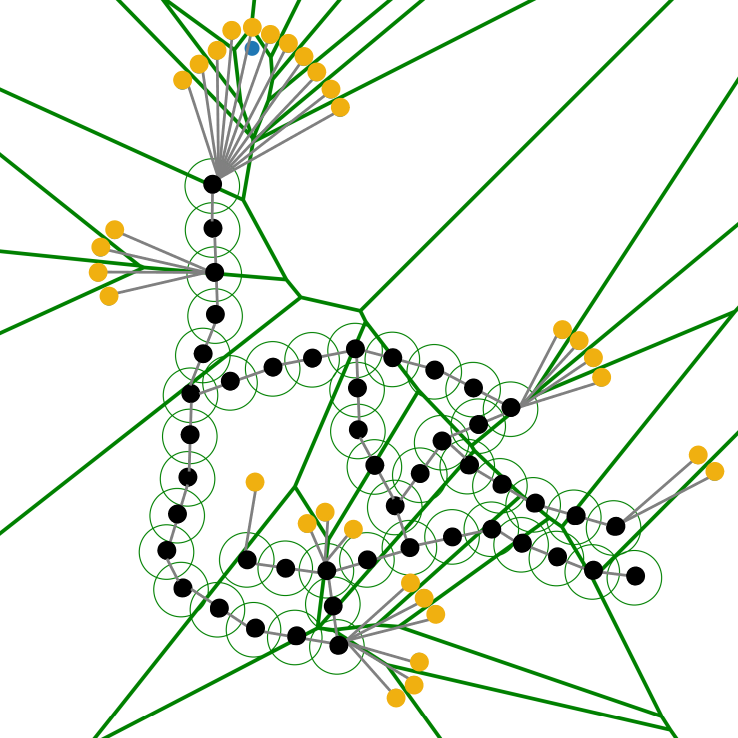
\includegraphics[width=.45\textwidth]{figures/irm_voronoi_combined.png}  \caption{Information gain heuristic.  Green circles around breadcrumbs indicate explored areas.  Green lines indicate limits of areas to compute expected information gain, for each frontier within it.}
  \label{fig:info_heuristic}
\end{figure}

\ph{Belief tree search overview}
We employ POMCP \cite{silver2010monte} for the belief tree search.
It basically uses Monte Carlo tree search (MCTS), but the $\epsilon$-greedy action selection is altered by the UCT algorithm by explicitly considering the number of visits during search.
It has several advantages for our problem compared to other tree search algorithms such as Q-learning \cite{watkins1992q} or RTDP \cite{barto1995learning}.
It has a low bias in action selection, so it can search for a wide set of branches of the tree, and it does not require admissible heuristic functions. % while it may converge more slowly.

\ph{Belief tree search details}
A brief description of the belief tree search algorithm is presented in Algorithm~\ref{alg:pomcp}.
A robot maintains a belief tree where each node represents a belief state and each edge represents a graph action by the robot. We define the root node of our tree as the node closest to the robot's current pose. The tree incrementally grows from the root node through four phases: selection, expansion, simulation, and backpropagation. During selection, successive child nodes are selected until a leaf node is reached. If this leaf node is not terminal, then one or more child nodes are created according to the available actions at the leaf node. In the simulation phase, the utility of the expanded node is estimated by performing the \emph{frontier rollout} policy. During backpropogation, all node rewards along the path are updated according to the rollout evaluation. The visit count is also updated accordingly. For more details, refer to \cite{silver2010monte}.

\begin{algorithm}[t!]
\caption{Belief Tree Search Algorithm}
\label{alg:pomcp}
\begin{algorithmic} 
  \STATE Start from the current belief state
  \WHILE{the planning time remains}
    \WHILE{the finite horizon or a terminal node is not yet reached}
      \STATE Select the best action that maximizes the value function but with some exploration bonus
      \STATE Get the successor node (from the IRM or a generative model)
      \STATE Add the new successor node to the tree
    \ENDWHILE
    \STATE Update the values and the number of visits by backpropagation from the leaf node to the root node
  \ENDWHILE
\end{algorithmic}
\end{algorithm}



\subsection{Grid-level Planning}

\ph{Map reward}
We implement the map reward function as:
\begin{align}
    R^M(b_t, \pi^M(b_t;v_j) = I(b_t,\pi^M) + \alpha_d d(x_t,v_j)
\end{align}
where we weigh the information gain with the distance from the goal $v_j$ with $\alpha_d$.

\ph{Risk Definition}
We define risk  $\rho(b_t,\pi^M(\cdot,\theta)) = \rho(v_i,\pi^M(\cdot,v_j))$ as the probability of failing to safely traverse from node $v_i$ to $v_j$.  To calculate this probability we compute the probability of safety traversing each cell in the map.  Within each grid cell, there may exist multiple risk factors.  Denote the number of risk factors as $n_\rho$.  Each risk factor may be due to a different source of potential failure, e.g. rough terrain, proximity to obstacles, slope, slippery/muddy terrain, etc.  We can then compute the probability of failing to traverse a cell $\rho_c(m^i)$ as:
\begin{align}
    \rho_c(m^i) = 1-\prod_{r=1}^{n_\rho} (1-\rho_r(m^i))
\end{align}
We then compute the risk of the entire path from node $v_i$ to node $v_j$ as the aggregate risk of traversing the cells along the path:
\begin{align}
    \rho(v_i,\pi^M(\cdot,v_j))=1-\prod_t^{t+\tau}(1-\rho_c(m^{i_t}))
\end{align}
which we want to constrain to be below some graph-level risk threshold $\psi(k)$.

\ph{Planner implementation}
To find the optimal path from node $v_i$ to $v_j$, we can optimize Eq. (\ref{eq:mapopt}) with any approximate method.  A wide range of approximations exist for solving the general information maximization problem.  A low fidelity approximation might be to reduce the problem to a simple $A^*$ search by finding the highest-reward path between node $v_i$ and $v_j$.  To disentangle the effect of updating the map belief after taking an action, we can make the approximation that the information to be gained at each grid cell is simply the number of unknown cells within the local sensing radius.  Then we can employ $A^*$ search on grid cells which are below a desired risk threshold.

\begin{figure}[t!]
  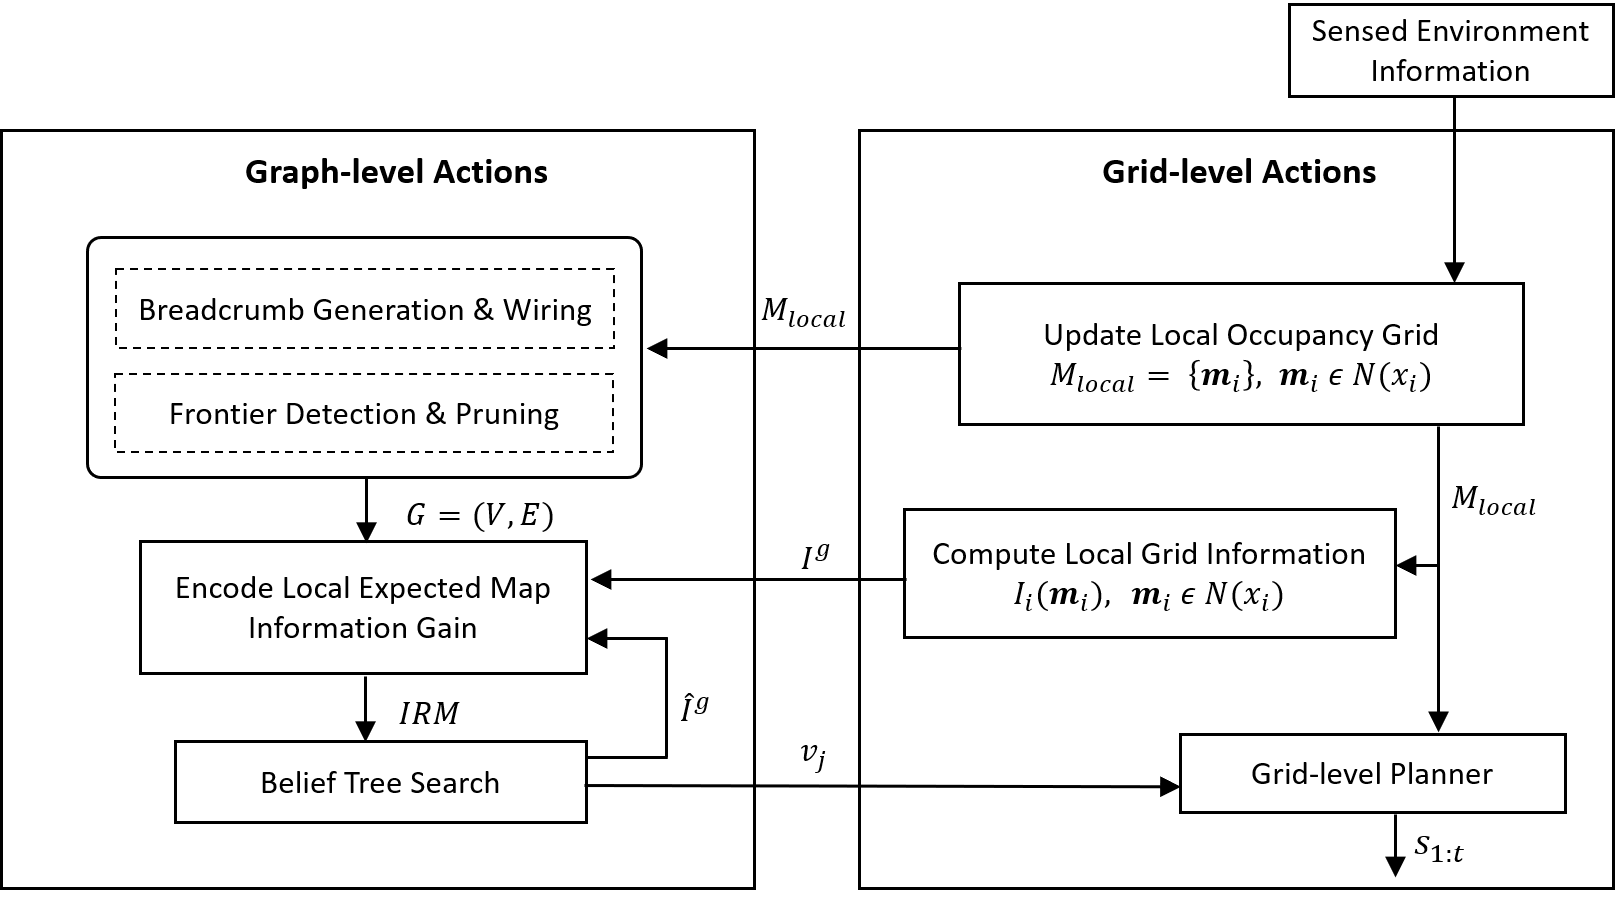
\includegraphics[width=.48\textwidth]{figures/structure_v5.png}
  \centering
  \caption{Hierarchical Information-based Planner Architecture}
  \label{fig:architecture}
\end{figure}

\section{Experimental Validation}\label{sec:urban}

\ph{CoRL expts}
\begin{enumerate}
    \item Sim (mission)
    \item toy example (rosbag expt)
    % \item Hardware test (Spot, Caltech outdoor garden)
\end{enumerate}

\ph{metrics}
\begin{itemize}
    \item Use metrics from monthly demos
\end{itemize}

We evaluated the proposed method during the Urban Circuit of the DARPA Subterranean Challenge in February 2020. Two multi-level courses (Alpha and Beta) were configured in an unfinished power plant station. A team of robots, comprising two quadraped Spot and two differential-drive wheeled Husky robots, were allowed one hour to explore each course. Below we present our multi-resolution exploration planner implemented during the Challenge. As a first iteration simplification, we classify graph planning as either local or global. 

\subsubsection{Local Graph-level policy}
The local graph-level policy maps the graph $G$ and node $v_i$ associated with the robot's current state to a frontier node $v_j$:
\begin{align}
  \pi^g: (G,v_i) \rightarrow v_j,~~ v_j \in F
\end{align}
We define the graph-level reward as:
\begin{align}
    J^{g}(v_i, \pi^g) &= \theta_{bearing}(v_i, I^g(v_i,\pi^g)) 
\end{align}
The output of a graph policy $\pi^g$ is a frontier node $v_j$. The expected information gain $I^g$ is evaluated by the creation of frontier nodes, and serves an an input to the cost of traversal function $\theta_{bearing}$. We use bearing angle, or the relative planar angle between the robot's heading direction and a frontier, as the graph-level cost as it is correlated with the time required to execute a graph policy. Specifically, graph policies (i.e. frontier goals) that minimize velocity changes are associated with lower execution times, and therefore are preferable.  

We then define the optimal graph policy as:
\begin{align}
    \pi^{g*} &= \arg\min_{\pi^g \in \Pi} J^{g}(v_i, \pi^g) \nonumber \\
    ~s.t.,~~~ & \rho(v_i,\pi^M(\cdot,v_j)) > \psi(t) \nonumber \\
    & |\theta_{bearing}(v_i, v_j)| < \pi/2 
    \label{eq:local_constraint}
\end{align}
where $\rho(v_i,\pi^M(\cdot,v_j))$ is the probability of a traversal between $v_i$ and $v_j$. While the first constraint ensures that the selected frontier is traversable, the latter constraint on the bearing angle $\theta_{bearing}(v_i, v_j)$ results in a depth-first exploration behavior. A global graph-level policy is adopted if no local graph-level policy exists satisfying these constraints

\subsubsection{Global Graph-level policy}
Frontier nodes are clustered according to the minimum number of edges connecting any two sets of observations through a hierarchical agglomerative clustering strategy. The number of frontiers in a cluster $F^d$ is denoted by $|F^d|$, and the minimum number of edges between a node $v_i$ and cluster $F^d$ is $n_E(v_i,F^d)$. 

The global graph-level policy maps the graph $G$ and node $v_i$ associated with the robot's current pose to the frontier node closest to the centroid of a frontier cluster $F^d$:
\begin{align}
  \pi^g&: (G,v_i) \rightarrow v_{j} \nonumber \\
  ~s.t.,~~~ &v_j= \arg\min_{v_j \in F} dist(v_{j}, centroid(F^d))
\end{align}
We define the graph-level information gain $I^g$ and cost $\tau$ for a graph-level policy as:
\begin{align}
    I^g(v_i,\pi^g) &= |F^d| \nonumber \\
    \tau(v_i,\pi^g) &= n_E(v_i,F^d) 
\end{align}
The expected information gain for a given graph policy is cluster size $|F^d|$ as it is indicative of an unexplored region's expanse. Then given a starting node $v_i$, we define the graph-level reward $J^g$ associated with a graph-level policy $\pi^g$ as: 
\begin{align}
    J^{g}(v_i, \pi^g) &= I^g(v_i,\pi^g) + \alpha~\tau(v_i,\pi^g)^{-1}
\end{align}
where $\alpha$ weighs the cost of traversal against new information gain for a given frontier cluster. We then define the optimal graph policy as:
\begin{align}
    \pi^{g*} &= \arg\min_{\pi^g \in \Pi} J^{g}(v_i, \pi^g) \nonumber
\end{align}

\subsubsection{Grid-level policy}
Within the grid-level policy $\pi^M$ we did not consider information gain directly.  Instead, we compute the risk of traversal for each grid cell via a traversability analysis which looks at ground surface normals and step height of obstacles.  It identifies lethal vs non-lethal regions which are then inflated by the footprint of the robot.  $A^*$ is used to plan low-risk paths between the robot's current position and the goal $\pi^g$.  The robot tracks this $A^*$ path with an underlying kinodynamic controller which samples trajectories in velocity space.

\subsubsection{Overall policy}
Given a graph-level policy, overall policy is:
\begin{align}
  \pi_t(G, v_j) = 
  \begin{dcases*}
    % \pi_t^{M*}(v_i, \pi^g(v_i)) & if $v_j \in \mathbb{N}(v_i)$ \\
    a_t^g(G, \pi^g(v_i)) & otherwise 
  \end{dcases*},
\end{align}
where $\mathbb{N}(v_i)$ denotes the neighborhood of the node $v_i$ associated with the robot's current state. $\pi_t^{M*}$ is an optimal policy in the map level given that the graph-level policy outputs a node $v_j$ in the neighborhood of $v_i$, and $a_t^G(G, v_i)$ is the shortest sequence of IRM edges to $v_j$.


\fi % COMMENTED







\section{Experimental Results}

\subsection{Experimental Setup}

baseline algorithms (name, approach, ...)

system config

experiment environment
- sim (AWS, ...)
- robot

...




Figure \ref{fig:beta_map} shows the map constructed during exploration of the Beta course. The ground floor of the course was mapped within 30 minutes.  

\begin{figure}[h!]
\centering
    \begin{tikzpicture}
	    \node[anchor=south west,inner sep=0] (image) at (0,0) {\includegraphics[width=0.48\textwidth]{figures/map_snapshots_combined_cropped.png}};
	    \begin{scope}[x={(image.south east)},y={(image.north west)}]
	    
	    	% Annotations
	    	\node [font=\scriptsize,above left,align=right,white] at (0.12,0.66) {1.8 min};
	    	\node [font=\scriptsize,above left,align=right,white] at (0.45,0.66) {3.6 min};
	    	\node [font=\scriptsize,above left,align=right,white] at (0.78,0.66) {6.6 min};
	    	\node [font=\scriptsize,above left,align=right,white] at (0.12,0.33) {9.6 min};
	    	\node [font=\scriptsize,above left,align=right,white] at (0.46,0.33) {14.4 min};
	    	\node [font=\scriptsize,above left,align=right,white] at (0.79,0.33) {15.6 min};
	    	\node [font=\scriptsize,above left,align=right,white] at (0.13,0.005) {24.6 min};
	    	\node [font=\scriptsize,above left,align=right,white] at (0.44,0.005) {27 min};
	    	\node [font=\scriptsize,above left,align=right,white] at (0.77,0.005) {60 min};
	    	
	        % helpers
	       % \draw[help lines,xstep=.1,ystep=.1] (0,0) grid (1,1);
	       % \foreach \x in {0,1,...,9} { \node [anchor=north] at (\x/10,0) {0.\x}; }
	       % \foreach \y in {0,1,...,9} { \node [anchor=east] at (0,\y/10) {0.\y}; }
	       
	    \end{scope}
	\end{tikzpicture}	
\caption{Sequential snapshots of map generated during exploration of Beta course during Urban Circuit of DARPA Subterranean Challenge. Four robots participated. An axis denotes each robot's location. The course runtime associated with each snapshot is given in the bottom left corner.} \label{fig:beta_map} 
\end{figure}


\begin{figure}[ht!]
  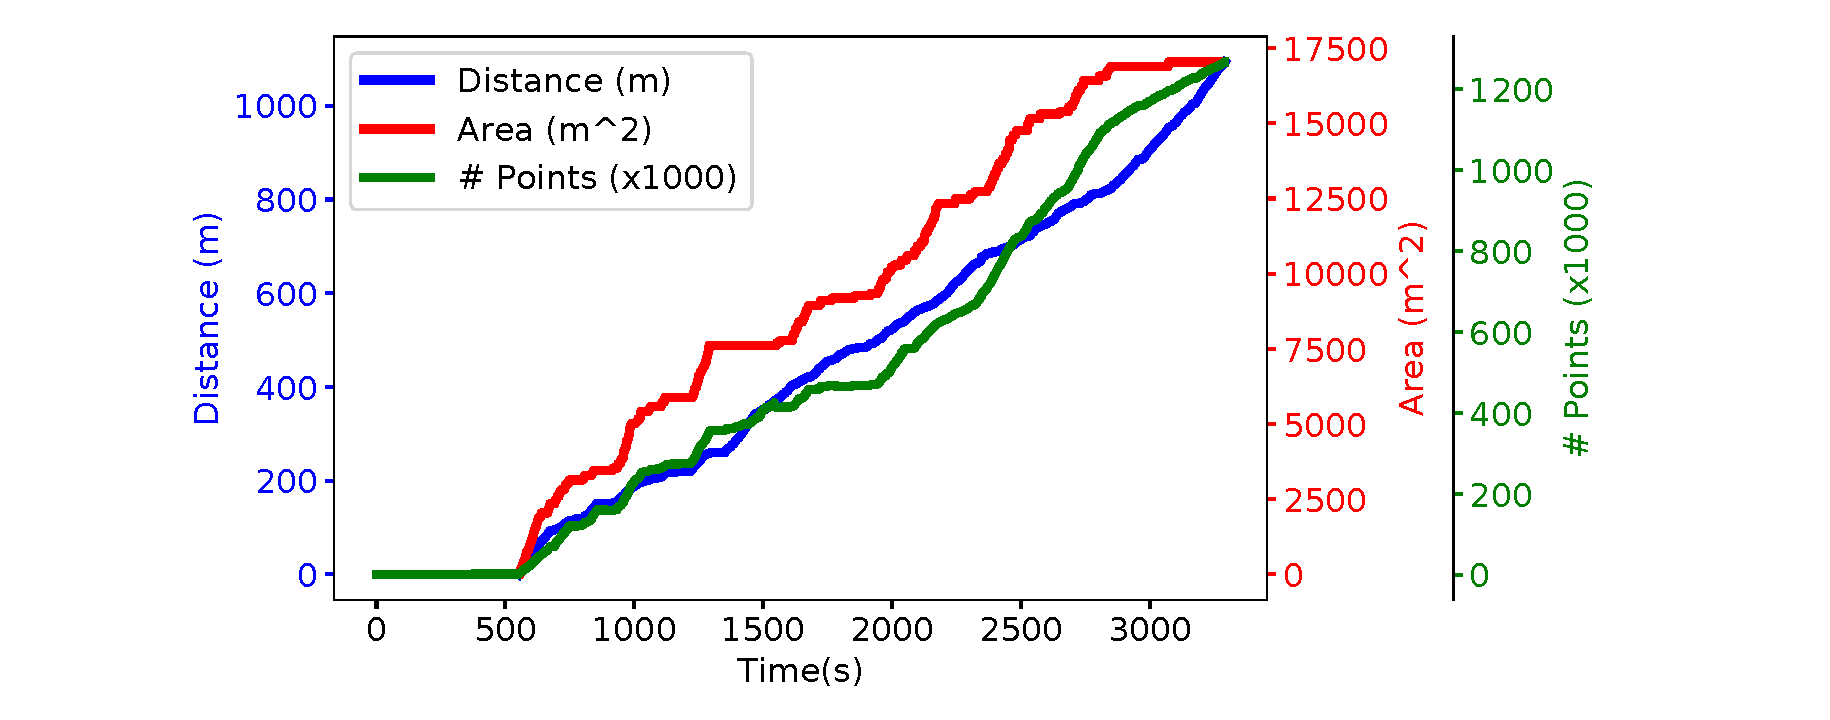
\includegraphics[width=.48\textwidth,trim=3cm 0 4cm 0, clip]{figures/dist_traveled.pdf}
  \centering
  \caption{Total distance traveled, total area covered, and total number of pointcloud points added to the 3D LiDAR map (at 10m resolution) vs.  time, during Team CoSTAR's second run on the Beta course in the DARPA Subterranean Challenge Urban Circuit.}
  \label{fig:dist_traveled}
\end{figure}

\begin{figure}[ht!]
  \includegraphics[width=.48\textwidth,angle=90]{figures/paths_on_map.png}
  \centering
  \caption{Overlay of paths traveled by robots over time on the ground truth pointcloud of the competition course.  Color indicates time at which the path was traversed, from purple ($t=0$) to yellow ($t=60min$).}
  \label{fig:paths_on_map}
\end{figure}


% \section{Old stuff, move to implementation}

% \begin{figure}[ht!]
%   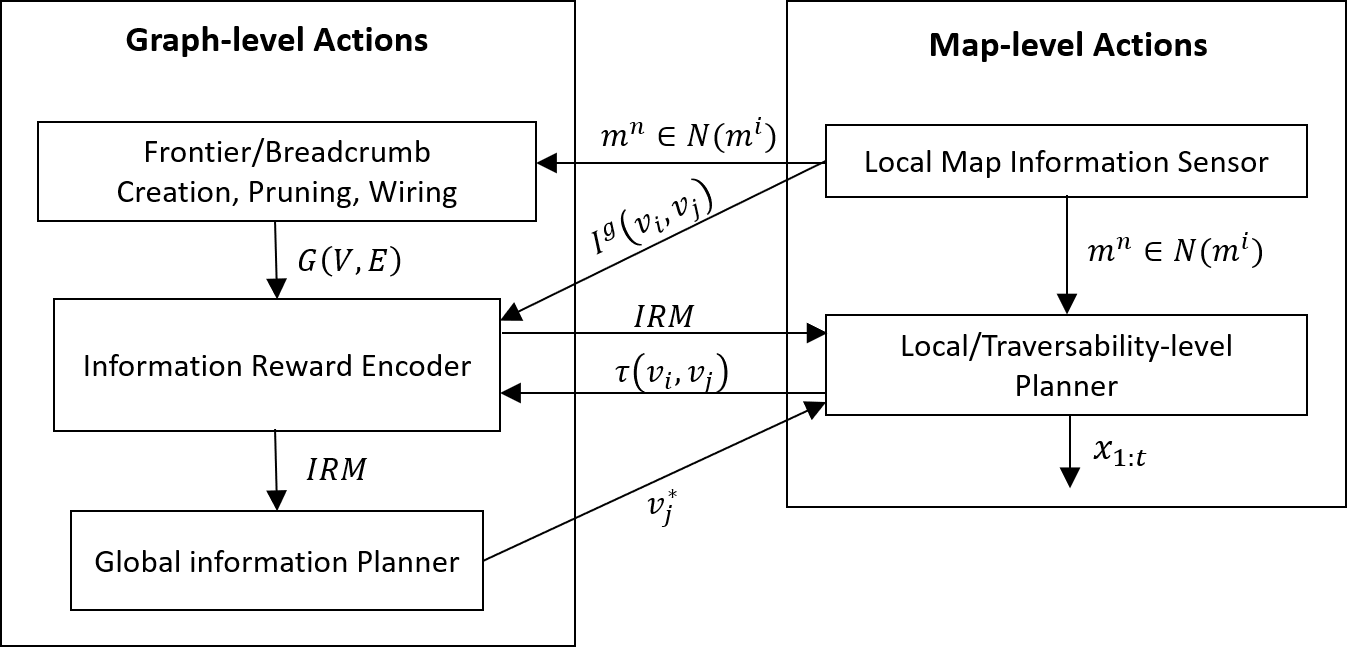
\includegraphics[width=.48\textwidth]{figures/structure_v3.png}
%   \centering
%   \caption{Implementation Architecture}
%   \label{fig:architecture}
% \end{figure}


% \ph{Defining expected value of frontiers (pt.2)}

% \begin{figure}[ht!]
%   \centering
%   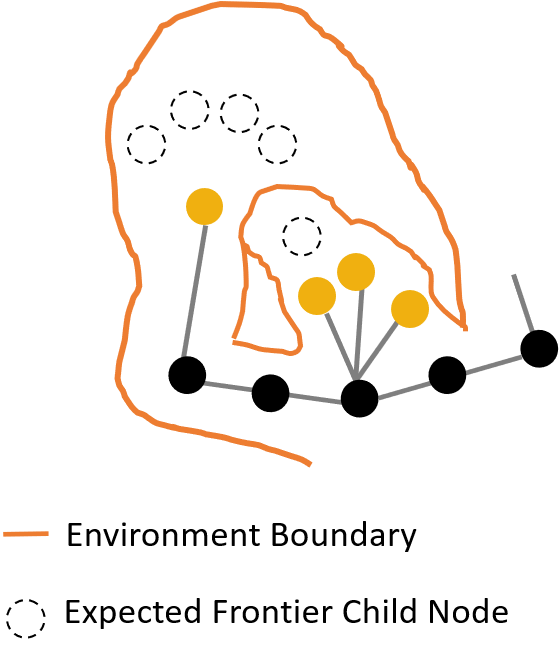
\includegraphics[width=.3\textwidth]{figures/irm_frontier_expected_value.png}
%   \caption{}
%   \label{fig:info_heuristic2}
% \end{figure}


% \ph{Possibly outdated}
% Our proposed framework is composed of receding-horizon planners in three hierarchical levels--graph, map, and traversability levels.
% Graph-level planning is conducted on the IRM, using the embedded information in its nodes and edges.
% Map-level planning uses a local occupancy grid map (20m$\times$20m) that is centered at the current robot pose.
% Traversability-level planning uses a smaller local occupancy grid map (5m$\times$5m) and the corresponding point cloud sensor data for the robot-specific traversability analysis.
% In order to ensure the robots continue autonomous exploration over time, we additionally impose a constraint regarding the risk level on each optimization problem.


% \subsubsection{Graph-level Receding-horizon Planning}

% \begin{align}
%   \pi_t^{G*}(b) &= \argmax_{\Pi_t^G} \mathbb{E} \left[ \frac{I^G(b; \pi_t^G(b))}{c_t^G(b; \pi_t^G(b))} \right]
%   \nonumber \\
%   s.t.~&~\rho_t^G(b; \pi_t^G(b))< \psi^G(t).
%   \label{eq:graphopt}
% \end{align}
% where $I^G(b; \pi_t^G(b))$ is the information gain in the graph level,
% $c_t^G(b; \pi_t^G(b))$ is a cost function that returns a time to execute an action under $\pi_t^G$.
% $\rho_t^G(b; \pi_t^G(b))$ is a risk measure for taking an action at $b$ under $\pi_t^G$, and
% $\psi^G(t)$ is a time-varying threshold for allowable risk at time $t$.
% (For example, $\psi^G(t)$ gets higher as $t$ gets closer to $T$, the total allowed time for exploration, in order to allow riskier actions.)

% \ph{Breadcrumb}
% Breadcrumb $x\in \mathbb{X}$ is a sampled state in the robot pose space. $C(x)\in M$ denotes a subset of the occupancy map comprised of cells in the radius $r$ of the breadcrumb $x$.

% \ph{Frontier}
% Breadcrumb $F\in \mathbb{X}$ is a sampled state in the robot pose space. $C(F)\in M$ denotes a subset of the occupancy map comprised of cells in the radius $r$ of the breadcrumb $F$.

% %\ph{Frontier cluster}

% \ph{Graph-level policy}
% We define the graph-level policy as follows.
% \begin{align}
%   \pi_t^G(b): (G,b) \rightarrow F^d
% \end{align}

% \begin{align}
%   \pi_t^G(b) = 
%   \begin{dcases*}
%     \pi_t^{M*}(b; F^d) & if $b \in C(F^d)$ \\
%     a_t^G(b; F^d) & otherwise 
%   \end{dcases*},
% \end{align}
% where $F^d$ is the desired frontier cluster (\todo{TODO: need more explanation}\!\!) based on $\pi_t^G$, and
% $\mathbb{N}(F^d)$ stands for the neighborhood belief states of $F^d$.
% $\pi_t^{M*}(b; F^d)$ is an optimal policy in the map level for $b$ given $F^d$, and
% $a_t^G(b; F^d)$ is an abstract graph-level action to reach $F^d$ following the shortest path IRM edges.
% \note{We may add another low-level optimization that solves for the concrete robot trajectory $x_{0:k}$ for the given $a_t^G$, which is effectively the mobility service in our implementation.}
% \hn{If the low-level service is already in operation, would it need to be modified function with this particular graph level policy?}


% \subsubsection{Local Information-gain Receding-horizon Planning}
% \todo{Bounded Map!}
% \begin{align}
%   \pi_t^{M*}(b; F^d) &= \argmax_{\Pi_t^M} \mathbb{E} \left[ \frac{I^M(b; \pi_t^M(b; F^d))}{c_t^M(b; \pi_t^M(b; F^d))} \right]
%   \nonumber \\
%   s.t.~&~\rho_t^M(b; \pi_t^M(b; F^d))< \psi^M(t).
%   \label{eq:mapopt}
% \end{align}
% where the notations are the same with Eq.~(\ref{eq:graphopt}) except that those with the superscript $M$ are for the map level.

% Similarly, we define the map-level policy as follows.
% \begin{align}
%   \pi_t^M(b; F^d) = \pi_t^{T*}(b; F^d, x^d),
% \end{align}
% where $x^d$ is the desired robot pose based on $\pi_b^M$.


% \subsubsection{Traversability-level Receding-horizon Planning}

% \begin{align}
%   \pi_t^{T*}(b; F^d, x^d)
%   &= \argmin_{\Pi_t^T} \mathbb{E} \left[ c^T(b; \pi_t^T(b; F^d, x^d)) \right]
%   \nonumber \\
%   s.t.~&~\rho_t^T(b; \pi_t^T(b; F^d, x^d))< \psi^T(t).
%   \label{eq:travopt}
% \end{align}
% where the notations are the same with Eq.~(\ref{eq:graphopt}) except that those with the superscript $T$ are for the traversability level.

% The traversability-level policy returns a desired robot trajectory $x_{t, 0:K}$, where the subscript $k$ denotes the time sub-step, dividing a single time step between $t$ and $t+1$ by $K$ sub-steps.

% The cost function in this level can be defined as follows.
% \begin{align}
%   c^T(b; \pi_t^T(b; F^d, x^d)) = c_l \sum_{k=0}^{K-1} d(x_k, x_{k+1}) + c_\rho \sum_{k=0}^K \rho_t^T(x_k),
% \end{align}
% where $d(x_k, x_{k+1})$ is a distance measure between two poses, $x_k$ and $x_{k+1}$.


% \todo{
% Things to do:
% \begin{enumerate}
%     \item Details of computing $I^E(v_i,\pi^G)$
%     \item Details of computing $I^V(v_j)$
%     \item How to compute risk $\rho$
%     \item Details of IRM planner implementation
%     \item Details of Local planner implementation
%     \item Details of Graph expansion
%     \item Details of 
% \end{enumerate}
% }



%%%%%%%%%%%%%%%%%%%%%%%%%%%%%%%%%%%%%%%%%%%%%%%%%%%%%%%%%%%%%%%%%%%%%%%%%%%%%%%%
\section{Conclusion}

In this work, we have developed a framework for exploring unknown environments in a POMDP framework in extremely large environments.  
To obtain a tractable solution we discretize the belief space into a robot and task-relevant graph structure which reduces our search space for good policies.  We call this graph structure an Information Roadmap (IRM).  We demonstrate these capabilites in the DARPA Subterranean Challenge.  Future work includes learning based methods for graph expansion information gain estimation, multi-robot policy search, and a richer incorporation of risk and time into the graph planning framework.




% \clearpage
% %%%%%%%%%%%%%%%%%%%%%%%%%%%%%%%%%%%%%%%%%%%%%%%%%%%%%%%%%%%%%%%%%%%%%%%%%%%%%%%%
% \section{Problem Formulation}
% Let $s$, $\pi_f$, and $M$ denote the robot's state, a move-to-frontier action, and map, respectively. We formulate the coverage objective function as the ratio of newly sensed map information ($B$) to the temporal cost of sensing this information ($c_t$), both of which are functions of the transition function $T(s,\pi_f,M)$.

% \begin{align}
%     J^{cov}(s,\pi_f,M) &= \frac{B[T(s,\pi_f,M)]}{c_t[T(s,\pi_f,M)]} \\ \nonumber \\ 
%     T &\colon s \times \pi_f \times M\to \tau \nonumber \\
%     B &\colon \tau\to \Delta n_{bc} \nonumber \\
%     c_t &\colon s \times \pi_f \times M\to \Delta t \nonumber 
% \end{align}

% \noindent where, for a given the move-to-frontier action $\pi_f$, $\tau$ is the robot trajectory, $\Delta t$ is duration of traversal, and $\Delta n_{bc}$ is the number of new breadcrumbs added to the IRM. We select an action $\pi_f$ which maximizes our coverage objective function:
% \begin{align}
%     % f^* &= \arg\max_{f\in F}_{~~\tau \in \Gamma} J^{cov}(s,f,M) \\
%     \pi_f^* &= \arg\max_{\substack{\pi_f\in \Pi_f \\ \tau \in T}} J^{cov}(s,f,M) \\
%     s.t.~~&~\textrm{risk}(s,\pi_f,M)< \psi(t)
% \end{align}

% \noindent The risk (or probability of traversal) associated with the optimal action is required to be smaller than a time adaptive threshold. As the duration of the mission progresses, the risk threshold $\psi(t)$ increases to allow for riskier actions.

% % Let $x_k$, $u_k$, and $z_k$ denote the robot state, action, and observation at the $k$-th time step.
% % \begin{align}
% %     \pi^* &= \arg\min_{\pi\in \Pi} J(?, ?, \pi) \\
% %     s.t.~~&~constraint 1 \\
% %     ~ &~constraint 2
% % \end{align}

% \subsection{Defining risk}
% It is easier to define risk as the probability of success, rather than the probability of failure, since for the mission to succeed, we require the intersection of multiple successful events.  Let $r(s,\pi_f,M,t)$ be the probability of success associated at each (timestep?  transition?), which we define as the probability that the robot does not fail or crash for that interval.  We define the total \emph{mission risk} $R$ as the probability that the robot does not fail over the entire mission.  For a given mission duration $D$, the mission risk is given by:
% \begin{equation}
%     R= \prod_{t=0}^D risk(s,\pi_f,M,t)
% \end{equation}
% In general, risk may be a function of the state $s$, actions $\pi_f$, and map $M$.  We can make the simplifying assumption that is is a function each grid cell within the map $m_i$.  (is $m_i$ the occupancy value or the grid itself?  or is $i$ indication the grid?)  Let $m_i(t)$ be the grid cell that the robot occupies at time $t$.  Then we have $risk(m_i(t)) = \prod_{k} r_k(m_i(t))$ where we have $k$ risk factors.  Each risk factor may be due to a different source of potential failure, e.g. rough terrain, proximity to obstacles, slope, slippery/muddy terrain, etc.  For computational tractability we can compute the log mission risk: 
% \begin{equation}
%     \log R=\bigg[\sum_{t=0}^D\sum_{k} \log(r_k(m_i(t)))\bigg] > \Phi
% \end{equation}
% which we want to constrain to be above some total acceptable mission risk threshold $\Phi$.
% \section{Problem Solution}

% \subsection{Local Selection}

% \begin{itemize}
%   \item Objective 1: Connect local to global coverage
%   \begin{itemize}
%   \item In-depth path planning to selected frontier
%   \item Expectation Model or leaf-node heuristic function
%   \end{itemize}
%   \item Objective 2: More robust traversability (no oscillations!)
%   \begin{itemize}
%   \item Way-point assignments 
%   \end{itemize}
% \end{itemize}


% %%%%%%%%%%%%%%%%%%%%%%%%%%%%%%%%%%%%%%%%%%%%%%%%%%%%%%%%%%%%%%%%%%%%%%%%%%%%%%%%
% \section{Environment representation}
% \subsection{Occupancy Grid Mapping}
% Given a set of observations taken at known robot poses, the posterior over maps is given by:
% \begin{align}
%     p(m | z_{1:t},x_{1:t})
% \end{align}
% \noindent where $m$ is the map, $z_{1:t}$ is the set of all measurements up to time $t$, and $x_{1:t}$ is path of robot. 
% Occupancy grid map is composed of grid cells:
% \begin{align}
%     m = \{\textbf{m}_i\}
% \end{align}
% \noindent where $\textbf{m}_i$ is associated with a binary occupancy value indicating whether cell is occupied or free. Calculating the posterior for every single map is intractable, therefore, problem can be formulated as the posterior over a single grid cell: 
% \begin{align}
%     p(\textbf{m}_i | z_{1:t},x_{1:t})
% \end{align}
% Here, we are estimating a fixed, binary state that does not change over time. When the state is static, posterior is only function of measurements:
% \begin{align}
%     p(\textbf{m}_i | z_{1:t},x_{1:t}) = p(\textbf{m}_i | z_{1:t})
%     \label{static}
% \end{align}
% This problem can be addressed by the Binary Bayes filter. The \emph{odds} of a state $\textbf{m}_i$ is defined as the ratio of the probability that the cell is free to that of the cell being occupied:
% \begin{align}
%     \frac{p(\textbf{m}_i | z_{1:t},x_{1:t})}{1-p(\textbf{m}_i | z_{1:t},x_{1:t})}
%     \label{odd}
% \end{align}
% The \emph{log odds} is the logarithm of this ratio:

% \begin{align}
%     l_{t,i} = \log\frac{p(\textbf{m}_i | z_{1:t},x_{1:t})}{1-p(\textbf{m}_i | z_{1:t},x_{1:t})}
%     \label{log_odd}
% \end{align}
% An inverse measurement model, $p(\textbf{m}_i | z_{1:t},x_{1:t})$, which specifies the distribution over the binary state variable $\textbf{m}_i$ as a function of the measurement $z_{1:t}$, is used since the measurements are much more complex than the binary state. 
% \noindent By rearranging Eq.~(\ref{log_odd}), the posterior over the grid cell is exposed:
% \begin{align}
%     p(\textbf{m}_i | z_{1:t},x_{1:t}) = 1-\frac{1}{1+\exp(l(\textbf{m}_i))}
% \end{align}
% \noindent Eq.~(\ref{log_odd}) can be expanded in accordance with Bayes filter:
% \begin{align}
%     l_{t,i} &= \log\frac{p(\textbf{m}_i | z_{1:t-1}, x_{1:t-1})}{1-p(\textbf{m}_i | z_{1:t-1}, x_{1:t-1})} + \log\frac{p(\textbf{m}_i | z_{t},x_{t})}{1-p(\textbf{m}_i | z_{t},x_{t})} \nonumber \\
%     &\quad - \log\frac{p(\textbf{m}_i)}{1-p(\textbf{m}_i)} \nonumber \\
%     &= l_{t-1,i} + \log\frac{p(\textbf{m}_i | z_{t},x_{t})}{1-p(\textbf{m}_i | z_{t},x_{t})} - l_{0,i}
% \end{align}
% \noindent where $l_{t-1,i}$ is the previous log-odds value, $l_{0,i}$ is the log-odds representation of the occupancy prior $p(\textbf{m}_i)$, and $p(\textbf{m}_i | z_{t},x_{t})$ is the inverse sensor model.

% However, this formulation does not reflect dependencies among neighboring cells. 

% \subsection{Information Gain}
% Entropy is a measure for the uncertainty of a posterior. The entropy $H_p(x)$ of a probability distribution $p$ is the expected information $E[-\log p]$. The entropy of the occupancy grid map posterior is
% \begin{align}
%     H_p(\textbf{m}_i) = -p(\textbf{m}_i) \log p(\textbf{m}_i) - (1-p(\textbf{m}_i)) \log(1-p(\textbf{m}_i))
% \end{align}
% \noindent and the expected entropy after measuring is $E[H_{p}(\textbf{m}_i)]$. Then the expected information gain when sensing a grid cell $\textbf{m}_i$ is: 
% \begin{align}
%     I_i = H_p(\textbf{m}_i) - E[H_{p}(\textbf{m}_i)]
% \end{align}



% \subsection{Receding-horizon Hierarchical Optimization}


% % We employ two strategies to solve our optimization problem; receding-horizon planning and hierarchical optimization.
% %
% % Due to the curse of history in POMDPs, the problem complexity increases exponentially with the planning horizon \cite{Pineau03}.
% % Receding-horizon planning is a common scheme to tackle such a challenge by interleaving execution and replanning for a finite horizon.
% %
% % Hierarchical optimization is also a useful methodology to solve large-scale problems in accordance with the divide-and-conquer paradigm.
% % \todo{TODO: add references for each.}

% Our proposed framework is composed of receding-horizon planners in three hierarchical levels--graph, map, and traversability levels.
% Graph-level planning is conducted on the IRM, using the embedded information in its nodes and edges.
% Map-level planning uses a local occupancy grid map (20m$\times$20m) that is centered at the current robot pose.
% Traversability-level planning uses a smaller local occupancy grid map (5m$\times$5m) and the corresponding point cloud sensor data for the robot-specific traversability analysis.
% In order to ensure the robots continue autonomous exploration over time, we additionally impose a constraint regarding the risk level on each optimization problem.


% \subsubsection{Graph-level Receding-horizon Planning}

% \begin{align}
%   \pi_t^{G*}(b) &= \argmax_{\Pi_t^G} \mathbb{E} \left[ \frac{I^G(b; \pi_t^G(b))}{c_t^G(b; \pi_t^G(b))} \right]
%   \nonumber \\
%   s.t.~&~\rho_t^G(b; \pi_t^G(b))< \psi^G(t).
%   \label{eq:graphopt}
% \end{align}
% where $I^G(b; \pi_t^G(b))$ is the information gain in the graph level,
% $c_t^G(b; \pi_t^G(b))$ is a cost function that returns a time to execute an action under $\pi_t^G$.
% $\rho_t^G(b; \pi_t^G(b))$ is a risk measure for taking an action at $b$ under $\pi_t^G$, and
% $\psi^G(t)$ is a time-varying threshold for allowable risk at time $t$.
% (For example, $\psi^G(t)$ gets higher as $t$ gets closer to $T$, the total allowed time for exploration, in order to allow riskier actions.)

% % \ph{Breadcrumb}
% % Breadcrumb $x\in \mathbb{X}$ is a sampled state in the robot pose space. $C(x)\in M$ denotes a subset of the occupancy map comprised of cells in the radius $r$ of the breadcrumb $x$.

% % \ph{Frontier}
% % Breadcrumb $F\in \mathbb{X}$ is a sampled state in the robot pose space. $C(F)\in M$ denotes a subset of the occupancy map comprised of cells in the radius $r$ of the breadcrumb $F$.

% %\ph{Frontier cluster}

% \ph{Graph-level policy}
% We define the graph-level policy as follows.
% \begin{align}
%   \pi_t^G(b): (G,b) \rightarrow F^d
% \end{align}

% \begin{align}
%   \pi_t^G(b) = 
%   \begin{dcases*}
%     \pi_t^{M*}(b; F^d) & if $b \in C(F^d)$ \\
%     a_t^G(b; F^d) & otherwise 
%   \end{dcases*},
% \end{align}
% where $F^d$ is the desired frontier cluster (\todo{TODO: need more explanation}\!\!) based on $\pi_t^G$, and
% $\mathbb{N}(F^d)$ stands for the neighborhood belief states of $F^d$.
% $\pi_t^{M*}(b; F^d)$ is an optimal policy in the map level for $b$ given $F^d$, and
% $a_t^G(b; F^d)$ is an abstract graph-level action to reach $F^d$ following the shortest path IRM edges.
% \note{We may add another low-level optimization that solves for the concrete robot trajectory $x_{0:k}$ for the given $a_t^G$, which is effectively the mobility service in our implementation.}


% \subsubsection{Local Information-gain Receding-horizon Planning}
% \todo{Bounded Map!}
% \begin{align}
%   \pi_t^{M*}(b; F^d) &= \argmax_{\Pi_t^M} \mathbb{E} \left[ \frac{I^M(b; \pi_t^M(b; F^d))}{c_t^M(b; \pi_t^M(b; F^d))} \right]
%   \nonumber \\
%   s.t.~&~\rho_t^M(b; \pi_t^M(b; F^d))< \psi^M(t).
%   \label{eq:mapopt}
% \end{align}
% where the notations are the same with Eq.~(\ref{eq:graphopt}) except that those with the superscript $M$ are for the map level.

% Similarly, we define the map-level policy as follows.
% \begin{align}
%   \pi_t^M(b; F^d) = \pi_t^{T*}(b; F^d, x^d),
% \end{align}
% where $x^d$ is the desired robot pose based on $\pi_b^M$.


% \subsubsection{Traversability-level Receding-horizon Planning}

% \begin{align}
%   \pi_t^{T*}(b; F^d, x^d)
%   &= \argmin_{\Pi_t^T} \mathbb{E} \left[ c^T(b; \pi_t^T(b; F^d, x^d)) \right]
%   \nonumber \\
%   s.t.~&~\rho_t^T(b; \pi_t^T(b; F^d, x^d))< \psi^T(t).
%   \label{eq:travopt}
% \end{align}
% where the notations are the same with Eq.~(\ref{eq:graphopt}) except that those with the superscript $T$ are for the traversability level.

% The traversability-level policy returns a desired robot trajectory $x_{t, 0:K}$, where the subscript $k$ denotes the time sub-step, dividing a single time step between $t$ and $t+1$ by $K$ sub-steps.

% The cost function in this level can be defined as follows.
% \begin{align}
%   c^T(b; \pi_t^T(b; F^d, x^d)) = c_l \sum_{k=0}^{K-1} d(x_k, x_{k+1}) + c_\rho \sum_{k=0}^K \rho_t^T(x_k),
% \end{align}
% where $d(x_k, x_{k+1})$ is a distance measure between two poses, $x_k$ and $x_{k+1}$.
% $c_l$ and $c_\rho$ are the weights for the path length and the risk measure, respectively.

% %%%%%%%%%%%%%%%%%%%%%%%%%%%%%%%%%%%%%%%%%%%%%%%%%%%%%%%%%%%%%%%%%%%%%%%%%%%%%%%%
% \section{Risk quantification}
% In this section, we discuss how we associate risk and cost values to a given trajectory in the environment.

% %%%%%%%%%%%%%%%%%%%%%%%%%%%%%%%%%%%%%%%%%%%%%%%%%%%%%%%%%%%%%%%%%%%%%%%%%%%%%%%%
% \section{Frontier-based Coverage Planning}

% \subsection{IRM}



% \subsection{Frontier Detection}

% \subsubsection{Frontier map}
% \todo{David} How we represent 3D lidar data in 2D frontier map
% \begin{itemize}
%     \item We want to capture traversability information here
%     \item We can include a full discussion about traversability analysis, computing risk metrics for traversal, and capturing known vs. unknown regions
%     \item We can fold in the current writeup on traversability here, then add additional risk/traversability metrics
% \end{itemize}
% \subsubsection{Frontier detection}
% \todo{Sung} Frontier detection algorithm


% \subsection{Frontier Maintenance}
% \todo{Sung} Frontier node maintenance details

% %%%%%%%%%%%%%%%%%%%%%%%%%%%%%%%%%%%%%%%%%%%%%%%%%%%%%%%%%%%%%%%%%%%%%%%%%%%%%%%%
% \section{Experiments}




% %%%%%%%%%%%%%%%%%%%%%%%%%%%%%%%%%%%%%%%%%%%%%%%%%%%%%%%%%%%%%%%%%%%%%%%%%%%%%%%%
% \section{Instructions}
% \ph{Paragraph header} Please start every single paragraph with a paragraph header, summarizing the intention of that paragraph. This is mainly for iterations during the paper preparation. We will remove most of them for the final report.

% %%%%%%%%%%%%%%%%%%%%%%%%%%%%%%%%%%%%%%%%%%%%%%%%%%%%%%%%%%%%%%%%%%%%%%%%%%%%%%%%
% \section{Introduction}
% \ph{Real world example} Consider a robot tasked to map a GPS-denied area in moving under time constraints. 

% %%%%%%%%%%%%%%%%%%%%%%%%%%%%%%%%%%%%%%%%%%%%%%%%%%%%%%%%%%%%%%%%%%%%%%%%%%%%%%%%
% \section{Problem Formulation}
% Let $x_k$, $u_k$, and $z_k$ denote the robot state, action, and observation at the $k$-th time step.


% %%%%%%%%%%%%%%%%%%%%%%%%%%%%%%%%%%%%%%%%%%%%%%%%%%%%%%%%%%%%%%%%%%%%%%%%%%%%%%%%
% \section{Map Representation}


% %%%%%%%%%%%%%%%%%%%%%%%%%%%%%%%%%%%%%%%%%%%%%%%%%%%%%%%%%%%%%%%%%%%%%%%%%%%%%%%%
% \section{Something of Map Posterior}

% %%%%%%%%%%%%%%%%%%%%%%%%%%%%%%%%%%%%%%%%%%%%%%%%%%%%%%%%%%%%%%%%%%%%%%%%%%%%%%%%
% \section{Planning}

% %%%%%%%%%%%%%%%%%%%%%%%%%%%%%%%%%%%%%%%%%%%%%%%%%%%%%%%%%%%%%%%%%%%%%%%%%%%%%%%%
% \section{Experiments}


% %%%%%%%%%%%%%%%%%%%%%%%%%%%%%%%%%%%%%%%%%%%%%%%%%%%%%%%%%%%%%%%%%%%%%%%%%%%%%%%%
% \section{Conclusion}



% % \section*{APPENDIX}


% %%%%%%%%%%%%%%%%%%%%%%%%%%%%%%%%%%%%%%%%%%%%%%%%%%%%%%%%%%%%%%%%%%%%%%%%%%%%%%%%
% \section{Background}

% \subsection{Partially Observable Markov Decision Process (POMDP)}

% %% (excerpted from Sung's thesis)

% In this section we briefly introduce generic POMDP formulation.
% For a detailed information, see e.g.,~\cite{Bertsekas05,TBF05,RN10}.

% Let $\mathbb{S}$, $\mathbb{A}$, and $\mathbb{Z}$ denote the state, action, and observation spaces, respectively.
% We denote the motion model $T(s, a, s') = P(s'\,|\,s, a)$, which defines the probability of being at state $s'$ after taking an action $a$ in state $s$.
% The observation model $Z(s, a, z) = P(z\,|\,s, a)$ is the probability of receiving observation $z$ after taking action $a$ in state $s$. 

% A belief $b(s)$ is a posterior distribution over all possible states given the past actions and observations, i.e., $b_{t}(s) = P(s \,|\, a_{0:t-1}, z_{1:t})$ where the subscript $t$ denotes the time step.
% Note that a POMDP problem can be formulated as a \textit{Belief MDP} by taking $b(s)$ as an MDP state, also referred to as a \textit{belief state} $b \in \mathbb{B}$, where $\mathbb{B}$ is referred to as \textit{belief space}.

% Given $a_{t-1}$, $z_t$, and $b_{t-1}(s)$,
% the updated belief $b_t(s)$ can be computed by Bayesian filtering, which can be divided into two sub-steps as follows.
% \begin{align}
%   b_{t-1}(s; a_{t-1}) &= \sum_{s' \in \mathbb{S}} T(s, a_{t-1}, s') b_{t-1}(s),
%   \label{eq:prediction}
%   \\
%   b_t(s; a_{t-1}, z_t) &= \eta Z(s, a_{t-1}, z_t) b_{t-1}(s; a_{t-1}),
%   \label{eq:correction}
% \end{align}
% where $\eta$ is a normalizing constant.
% % For notational convenience, let us denote $b_{t-1}(s; a) = b_{t-1}^a$ and $b_t(s; a, z) = b_t = b_{t-1}^{a z}$ hereafter.

% A policy $\pi : \mathbb{B} \rightarrow \mathbb{A}$ maps each belief state $b$ to a desirable action $a$.
% The expected cost of an action for the true state can be represented as a cost function in a belief space, $c(b, a) \in \mathbb{R}^+$.
% Given a policy $\pi$ and a belief $b \in \mathbb{B}$, we can compute the value function,
% \begin{align}
%   J(b; \pi) = \mathbb{E} \left[ \sum_{t=0}^\infty \gamma^t c(b_t, \pi(b_t)) \right]\!,
%   \label{eq:trueV}
% \end{align}
% where $b_0$ is the initial belief state and 	$\gamma \in (0, 1]$ is a discount factor that reduces the effect of later costs.


% We can rewrite Eq.~(\ref{eq:trueV}) in a recursive form, which is called the Bellman equation.
% \begin{align}
% J(b; \pi) = c(b^i, \pi(b)) % \nonumber \\
%   + \gamma \sum_{b' \in \mathbb{B}} \tau(b, \pi(b), b') J(b'; \pi),
%   \label{eq:bellman}
% \end{align}
% where $\tau(b, \pi(b), b') = \sum_{z \in \mathbb{Z}} P(b'|b,\pi(b),z) P(z|b,\pi(b))$ is the transition probability from $b$ to $b'$ under $\pi$,
% which can be derived from Eq.~(\ref{eq:prediction}) and~(\ref{eq:correction}).
% For further details, see~\cite{Ross08}.

% It is often convenient to define the so-called Q-value function for an intermediate belief-action pair, $(b, a)$ or simply $b^a$, as follows.
% \begin{align}
%   Q(b^a; \pi) =\; & c(b, a) + \gamma \sum_{b' \in \mathbb{B}} \tau(b, a, b') J(b'; \pi).
%   \label{eq:qfunction}
% \end{align}
% Then Eq.~(\ref{eq:bellman}) can be written as follows.
% \begin{align}
% J(b; \pi) =\; & \min_{a \in \mathbb{A}} Q(b, a; \pi)
% \label{eq:minq}
% \end{align}

% We now restate our POMDP problem as an optimization problem.
% \begin{align}
%   \pi^*(b) & = \argmin_{\Pi_{0:\infty}} \mathbb{E} \left[ \sum_{t=0}^\infty \gamma^t c(b_t, \pi_t(b_t)) \right]
%   \nonumber \\ 
%   &  = \argmin_{\Pi_{0:\infty}} J(b_t; \pi_t).
%   \label{eq:pomdpopt}
% \end{align}


% \subsection{Occupancy Grid Mapping}

% An occupancy grid map is a discretized random field in multi-dimensional space, where each independent cell stores a probabilistic estimate of its occupancy state \cite{moravec1985high,elfes1990stochastic}.
% %
% Formally, an occupancy grid map is composed of grid cells:
% \begin{align}
%   M = (\mathbf{m}^1, \mathbf{m}^2, \dots, \mathbf{m}^{N_M}),
% \end{align}
% where $\mathbf{m}^i$ is a Bernoulli random variable for the binary occupancy state of the $i$-th cell,
% i.e., $\mathbf{m}^i \in \{occupied, free\}$, and
% $N_M$ is the total number of grid cells in the map.
% The value of $\mathbf{m}^i$ is often assumed to be static over time.
% \note{We can augment further grid cell attributes, such as traversability.}

% Occupancy grid mapping is to compute the posterior probability of occupancy of the whole map $M$, given the observations $z_{1:t}$ and robot trajectory $x_{1:t}$ up to time $t$:
% \begin{align}
%   p(M | z_{1:t}, x_{1:t}).
% \end{align}
% Unfortunately, it is usually intractable to compute directly from $M$ due to its complexity of $2^{|M|}$.
% So, it is often to assume the occupancy grid map to be a Markov random field of order 0 in which the occupancy probability of each grid cell is independent \cite{TBF05,elfes1990stochastic}.
% With the cell independence assumption, $p(M | z_{1:t}, x_{1:t})$ can be determined from the individual cell state probability, $p(\mathbf{m}^i | z_{1:t}, x_{1:t})$.

% Given a sensor model $p(z | \mathbf{m}^i, x)$, this probability can be computed recursively as follows.
% \begin{align}
%   p(\mathbf{m}^i | z_{1:t}, x_{1:t}) =
%   \frac{p(z_t | \mathbf{m}^i, x_{t}) p(\mathbf{m}^i | z_{1:t-1}, x_{1:t-1})}
%       {\sum_{\forall j} p(z_t | \mathbf{m}^j, x_{t}) p(\mathbf{m}^j | z_{1:t-1}, x_{1:t-1})}.
% \end{align}
% Note that the sensor model $p(z | \mathbf{m}^i, x)$ can be quite complex as it should consider all possible grid configurations.
% Thus, it is often handled by maximum likelihood estimation or Rao-Blackwellized particle filtering methods \cite{burgard2005coordinated,stachniss2005information}.

% Entropy can be used as a measure for the uncertainty of random variables.
% The entropy $H_p(x)$ of a probability distribution $p$ is the expected information, defined as $\mathbb{E}_p[-\log p(x)]$ \cite{cover2012elements}.
% The entropy of the occupancy state of the $i$-th cell can be written as follows.
% \begin{align}
%   H_p(\mathbf{m}^i) = -p_o \log_2 p_{o} - p_f \log_2 p_f,
% \end{align}
% where $p_o = p(\mathbf{m}^i = occupied)$ and $p_f = p(\mathbf{m}^i = free) = 1 - p_o$.
% If a grid cell is unknown for its occupancy with the initial prior of $p_o = p_f = 0.5$, $H_p(\mathbf{m}^i) = 1$, and if it is fully known to be either occupied or free, $H_{p}(\mathbf{m}^i) = 0$.
% %
% Then, under the cell independence assumption, the total entropy of the map $M$ is
% \begin{align}
%   H_p(M) = \textstyle \sum_{i = 1}^N H_{p}(\mathbf{m}^i).
% \end{align}

% Now we can introduce information gain $I^i$ obtained from a new observation $z_t$ and its corresponding robot pose $x_t$~\cite{cover2012elements}.
% \begin{align}
%   I^i(\mathbf{m}^i, z_t, x_t) = H_p(\mathbf{m}^i | z_{1:t-1}, x_{1:t-1}) - H_p(\mathbf{m}^i | z_{1:t}, x_{1:t}).
% \end{align}
% Similarly, we can compute the \textit{expected} information gain for an action $a_t \in \mathbb{A}$ in the planning phase, by averaging over all possible observations.
% \begin{align}
%   &\hat{I}^i(\mathbf{m}^i; a_t)
%   = \mathbb{E}_{z_{t+1}, x_{t+1}} [ I^i (\mathbf{m}^i, z_{t+1}, x_{t+1}; a_t) ] \nonumber \\
%   &\!\!= H_p(\mathbf{m}^i | z_{1:t}, x_{1:t}) - \mathbb{E}_{z_{t+1}, x_{t+1}} [ H_p (\mathbf{m}^i | z_{1:t+1}, x_{1:t+1}) ].
% \end{align}

% The total information gain from a scanning sensor can be computed from local updates as follows
% \cite{bourgault2002information}.
% \begin{align}
%   I(M, z_t, x_t) = \sum_{i \in S_t} I^i(\mathbf{m}^i, z_t, x_t),
%   \label{eq:infogain}
% \end{align}
% where $S_t$ is a set of indices of the grid cells within the region of sensor coverage at time $t$, which would depend on $x_t$.


% \subsection{EXTRA}
% \begin{align}
%   J(b;\pi) &= \mathbb{E} \left[ \sum_{t=0}^\infty \gamma^t I(b_t; \pi_t(b_t)) \right], \label{eq:artifactopt_cost}\\
%   \pi^*(b) & = \argmax_{\Pi} J(b;\pi), \label{eq:artifactopt}\\
%   J^*(b) &= \max_{\Pi} J(b;\pi) , \label{eq:artifactopt_value}
% \end{align}

% % \note{Here, we do not explicitly include the localization accuracy in the objective function, unlike some of SLAM formulations. If anyone has a good idea how to describe this, please feel free to contribute.}

% where $J(b;\pi)$ is the value function and $J^*(b)$ is the optimal value function.  Traditionally, this problem can be solved at each timestep using a dynamic programming approach, which decomposes the maximization over an infinite number of timesteps to a maximization over one timestep at a time.  We can rewrite Eq.~(\ref{eq:artifactopt_value}) in a recursive form, which is called the optimal Bellman equation.
% \begin{align}
% J^*(b) = \max_{\Pi} \left[I(b, \pi(b)) % \nonumber \\
%   + \gamma \sum_{b' \in \mathbb{B}} \tau(b, \pi(b), b') J^*(b')\right],
%   \label{eq:bellman_opt}
% \end{align}
% where $\tau(b, \pi(b), b') = \sum_{z \in \mathbb{Z}} P(b'|b,\pi(b),z) P(z|b,\pi(b))$ is the transition probability from $b$ to $b'$ under $\pi$,
% which can be derived from Eq.~(\ref{eq:prediction}) and~(\ref{eq:correction}) (For further details, see~\cite{Ross08}).  At each timestep we have the optimal policy in terms of the optimal value $J^*$:
% \begin{align}
% \pi^*(b) = \argmax_{\Pi} \left[I(b, \pi(b)) % \nonumber \\
%   + \gamma \sum_{b' \in \mathbb{B}} \tau(b, \pi(b), b') J^*(b')\right].
%   \label{eq:bellman_opt_policy}
% \end{align}

% The maximization is over one transition from $b$ to $b'$ rather than the entire infinite horizon, as long as we have an accurate $J^*$. For smaller problems, finding $J^*$ may be feasible via Monte-Carlo search or other exhaustive methods \todo{cite}.  

% To obtain a tractable... we discretize the belief $b=p(M,x)$.  In the next section we discretize the map $M$ with an occupancy grid map, and later we discuss discretizing $x\in\mathcal{S}$ by sampling, which we call Information Roadmap (IRM)...

% \subsection{EXTRA from Information Roadmap Planner}

% We restrict $\Pi$ to the set of policies defined by:
% \begin{align}
%     \Pi \triangleq \{\pi:V\rightarrow\mathbb{A}^\tau | \pi = \pi^M(\pi^g(v)),v\in V\}
% \end{align}
% where $\pi^g(v):V\rightarrow V$ \todo{extend to parameter} is a node-to-node graph policy within a class of node-to-node policies $\Pi^g$, and $\pi^M(v):V\rightarrow \mathbb{A}^\tau$ is local planner policy.  

% $\pi(v_i):V\rightarrow \mathbb{A}^\tau$ within a class of policies $\Pi$ which produces a sequence of map-level actions $\{a_t\}_{t=0}^\tau, a_t\in\mathbb{A}\forall t$.
% \begin{align}
%     \pi: b\rightarrow a\\
%     \pi(b,v) = \pi^M(b; \pi^g(v))
% \end{align}
% \todo{change output of graph-level policy to be another policy, also change to lowercase}
% We define a integrated/holistic-level policy $\pi(v_i):V\rightarrow \mathbb{A}^\tau$ within a class of policies $\Pi$ which produces a sequence of map-level actions $\{a_t\}_{t=0}^\tau, a_t\in\mathbb{A}\forall t$.  
% (In abuse of notation , $\tau$ can change.)  

% We restrict $\Pi$ to the set of policies defined by:
% \begin{align}
%     \Pi \triangleq \{\pi:V\rightarrow\mathbb{A}^\tau | \pi = \pi^M(\pi^g(v)),v\in V\}
% \end{align}
% where $\pi^g(v):V\rightarrow V$ \todo{extend to parameter} is a node-to-node graph policy within a class of node-to-node policies $\Pi^g$, and $\pi^M(v):V\rightarrow \mathbb{A}^\tau$ is local planner policy.  
% The target node $v_j$ is sent to the local planner policy.  

% \ph{Graph expansion information reward}
% We define the information gain from reaching a node $v_j$ as:
% \begin{align}
%     % I^G(v_i,v_j) = \sum_{s\in e_{ij}} I(s,\pi^M(s)) \\
%     I^V(v_j) = I^{future}(v_j)
% \end{align}
% where $I^{future}(v_j)$ is the expected future information gain which results from future actions after reaching the node, resulting from potential future information gain which results from potentially adding new nodes to the graph upon reaching that node.

% %\todo{information gain vs expected information - make sure this is consistent with background info}

% \ph{Graph action (total) reward}
% This is the total reward for having reached node $v_i$, then executing a single graph traversal action $\pi^G(v_i)$:
% \begin{multline}
%     I^G(v_{i}, \pi^G(v_{i})) = I^E(v_{i}, \pi^G(v_{i})) + \\
%     I^V(v_i) - \alpha c^E(v_i,\pi^G(v_i)) 
% \end{multline}
% \begin{multline}
%     R^G(v_{i}, \pi^G(v_{i})) = I^E(v_{i}, \pi^G(v_{i}))
%     - \alpha c^E(v_i,\pi^G(v_i)) 
% \end{multline}
% where $\alpha$ is some constant which trades off information gain with the cost of traversal.

% %%%%%%%%%%%%%%%%%%%%%%%%%%%%%%%%%%%%%%%%%%%%%%%%%%%%%%%%%%%%%%%%%%%%%%%%%%%%%%%%
% \section{Conclusion}


% \todo{Exponential rather than summed reward function? See [Navigation Strategies for Exploring Indoor Environments, H. H. Gonzalez-Banos and J.-C. Latombe, 2002], [Visual Saliency–aware Receding Horizon Autonomous Exploration with Application to Aerial Robotics, Tung Dang, Christos Papachristos, Kostas Alexis, 2018], [Receding Horizon “Next–Best–View” Planner for 3D Exploration, Andreas Bircher, Mina Kamel , Kostas Alexis , Helen Oleynikova, and Roland Siegwart, 2016]}

%\todo{information gain vs expected information - make sure this is consistent with background info}

% \ph{Graph action (total) reward}
% This is the total reward for having reached node $v_i$, then executing a single graph traversal action $\pi^G(v_i)$:
% \begin{multline}
%     I^G(v_{i}, \pi^G(v_{i})) = I^E(v_{i}, \pi^G(v_{i})) + \\
%     I^V(v_i) - \alpha c^E(v_i,\pi^G(v_i)) 
% \end{multline}
% \begin{multline}
%     R^G(v_{i}, \pi^G(v_{i})) = I^E(v_{i}, \pi^G(v_{i}))
%     - \alpha c^E(v_i,\pi^G(v_i)) 
% \end{multline}
% where $\alpha$ is some constant which trades off information gain with the cost of traversal.

% \ph{Graph Cost-to-go (Utility Function)}
% We define the cost-to-go as the sum of future expected information gain on the graph:
% \begin{align}
%   J^G(v_{0};\pi^G) &= \mathbb{E} \left[ \sum_{k=0}^\infty R^G(v_{k}, \pi^G(v_{k}))\right], \label{eq:artifactopt_cost}
% \end{align}



% %%%%%%%%%%%%%%%%%%%%%%%%%%%%%%%%%%%%%%%%%%%%%%%%%%%%%%%%%%%%%%%%%%%%%%%%%%%%%%%%
% \section{Questions}
% \begin{itemize}
%     \item what is the best map representation (continuous/grid)
%     \item what is the best representation for "occupancy" in the map - is it (free/unknown/occupied) vs risk (0,1)?  also include artifact presence or probability of artifact presence.
%     \item robot pose 3d? yaw?  quaternion?
%     \item information gain - how to interpret in IRM level?  total number of breadcrumbs?
%     \item 
% \end{itemize}

% \subsection{information gain brainstorming}
% \begin{itemize}
%     \item \# of breadcrumbs
%     \item 2d number of cells
%     \item 3d number voxels
%     \item mesh \# facets, surfaces (observed)
%     \item volume in 3d..
%     \item area of raytrace, area of coverage...
% \end{itemize}
% eventually we want to abstract this into IRM level.  need a happy marriage between high res info with irm abstraction.\\

% \subsection{How to decouple problem}
% \begin{itemize}
%     \item \# new breadcrumbs (current implementation)
%     \item 
% \end{itemize}

% %%%%%%%%%%%%%%%%%%%%%%%%%%%%%%%%%%%%%%%%%%%%%%%%
% \section{High-level instructions}
%
% \begin{verbatim}
%
% 1. What is the problem?
% 2. Why is it relevant?
% 3. Why is it hard?
% 4. What have others done?
% 5. What is missing?
% 6. What is our ONE key insight?
% 7. How do we compare against the state of the art?
% 8. What are our contributions?
% 9. What are our limitations?  
%
% @ Contribution
% - frontier-based autonomous exploration in large-scale unknown environments
%   : sparse-yet-informative graph representation of space for large-scale exploration
%     . resilient to localization error, loop closure, etc.
%     . abstract representation for less memory usage and easier data transfer
%   : frontier-based exploration in the real world
%     . frontier detection/filtering/pruning in complex 3D environment
%     . frontier-based coverage planner, aware of robot's traversability
%
% @ Structure
% - introduction
% - frontiering
%   : IRM - graphical space representation
%   : frontier segment detection
%   : frontier node sampling/filtering/pruning
% - coverage planner
%   : problem formulation
%   : local search
%   : global search
% - experimental results
% - conclusion
%
% \end{verbatim}
% \clearpage{}


%===============================================================================

% The maximum paper length is 8 pages excluding references and acknowledgements, and 10 pages including references and acknowledgements

\clearpage
% The acknowledgments are automatically included only in the final version of the paper.
\acknowledgments{If a paper is accepted, the final camera-ready version will (and probably should) include acknowledgments. All acknowledgments go at the end of the paper, including thanks to reviewers who gave useful comments, to colleagues who contributed to the ideas, and to funding agencies and corporate sponsors that provided financial support.}

%===============================================================================

% no \bibliographystyle is required, since the corl style is automatically used.
\textcolor{red}{CHECK REFERENCE FORMAT}
\bibliography{references}  % .bib


% IEEE / before CoRL
% \bibliographystyle{unsrt}
% \bibliography{references}


%%%%%%%%%%%%%%%%%%%%%%%%%%%%%%%%%%%%%%%%%%%%%%%%%%%%%%%%%%%%%%%%%%%%%%%%%%%%%%%%
%%%%%%%%%%%%%%%%%%%%%%%%%%%%%%%%%%%%%%%%%%%%%%%%%%%%%%%%%%%%%%%%%%%%%%%%%%%%%%%%
%%%%%%%%%%%%%%%%%%%%%%%%%%%%%%%%%%%%%%%%%%%%%%%%%%%%%%%%%%%%%%%%%%%%%%%%%%%%%%%%


% \clearpage{}
% \begin{figure}[H]
%   \centering
%   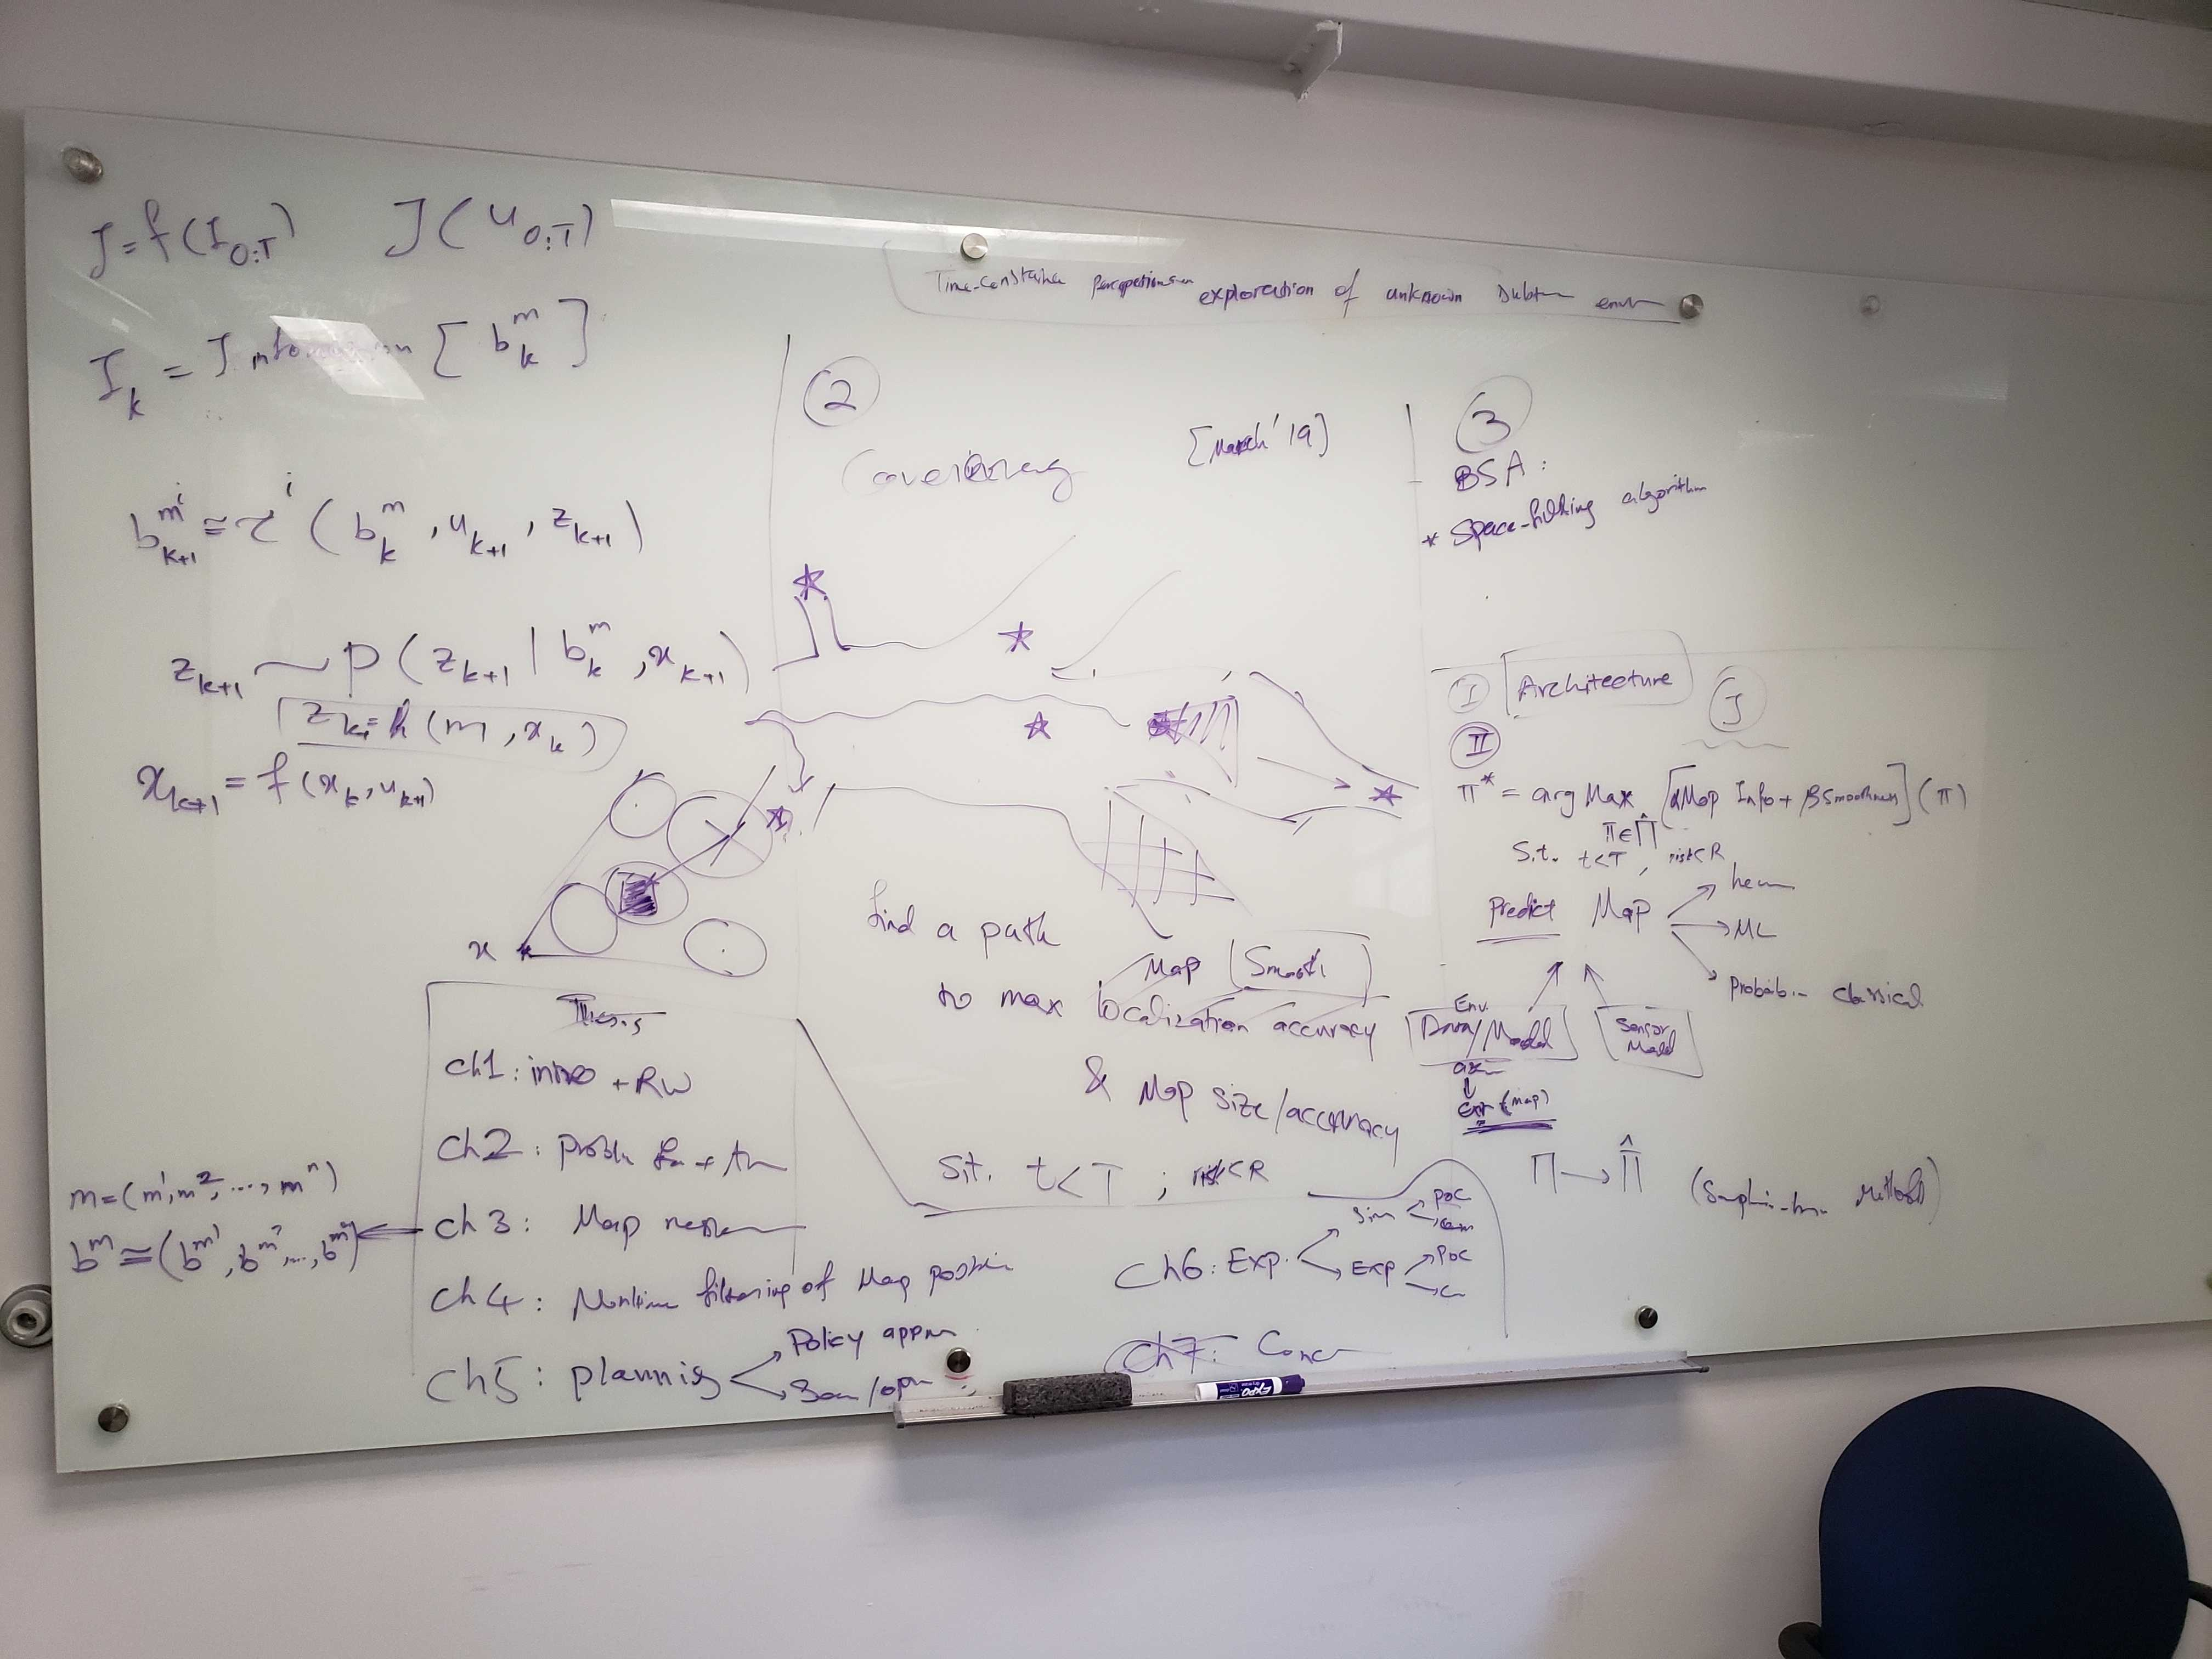
\includegraphics[width=.5\textwidth]{figures/whiteboard1.jpg}
%   \label{fig:whiteboard1}
% \end{figure}

% \begin{figure}[H]
%   \centering
%   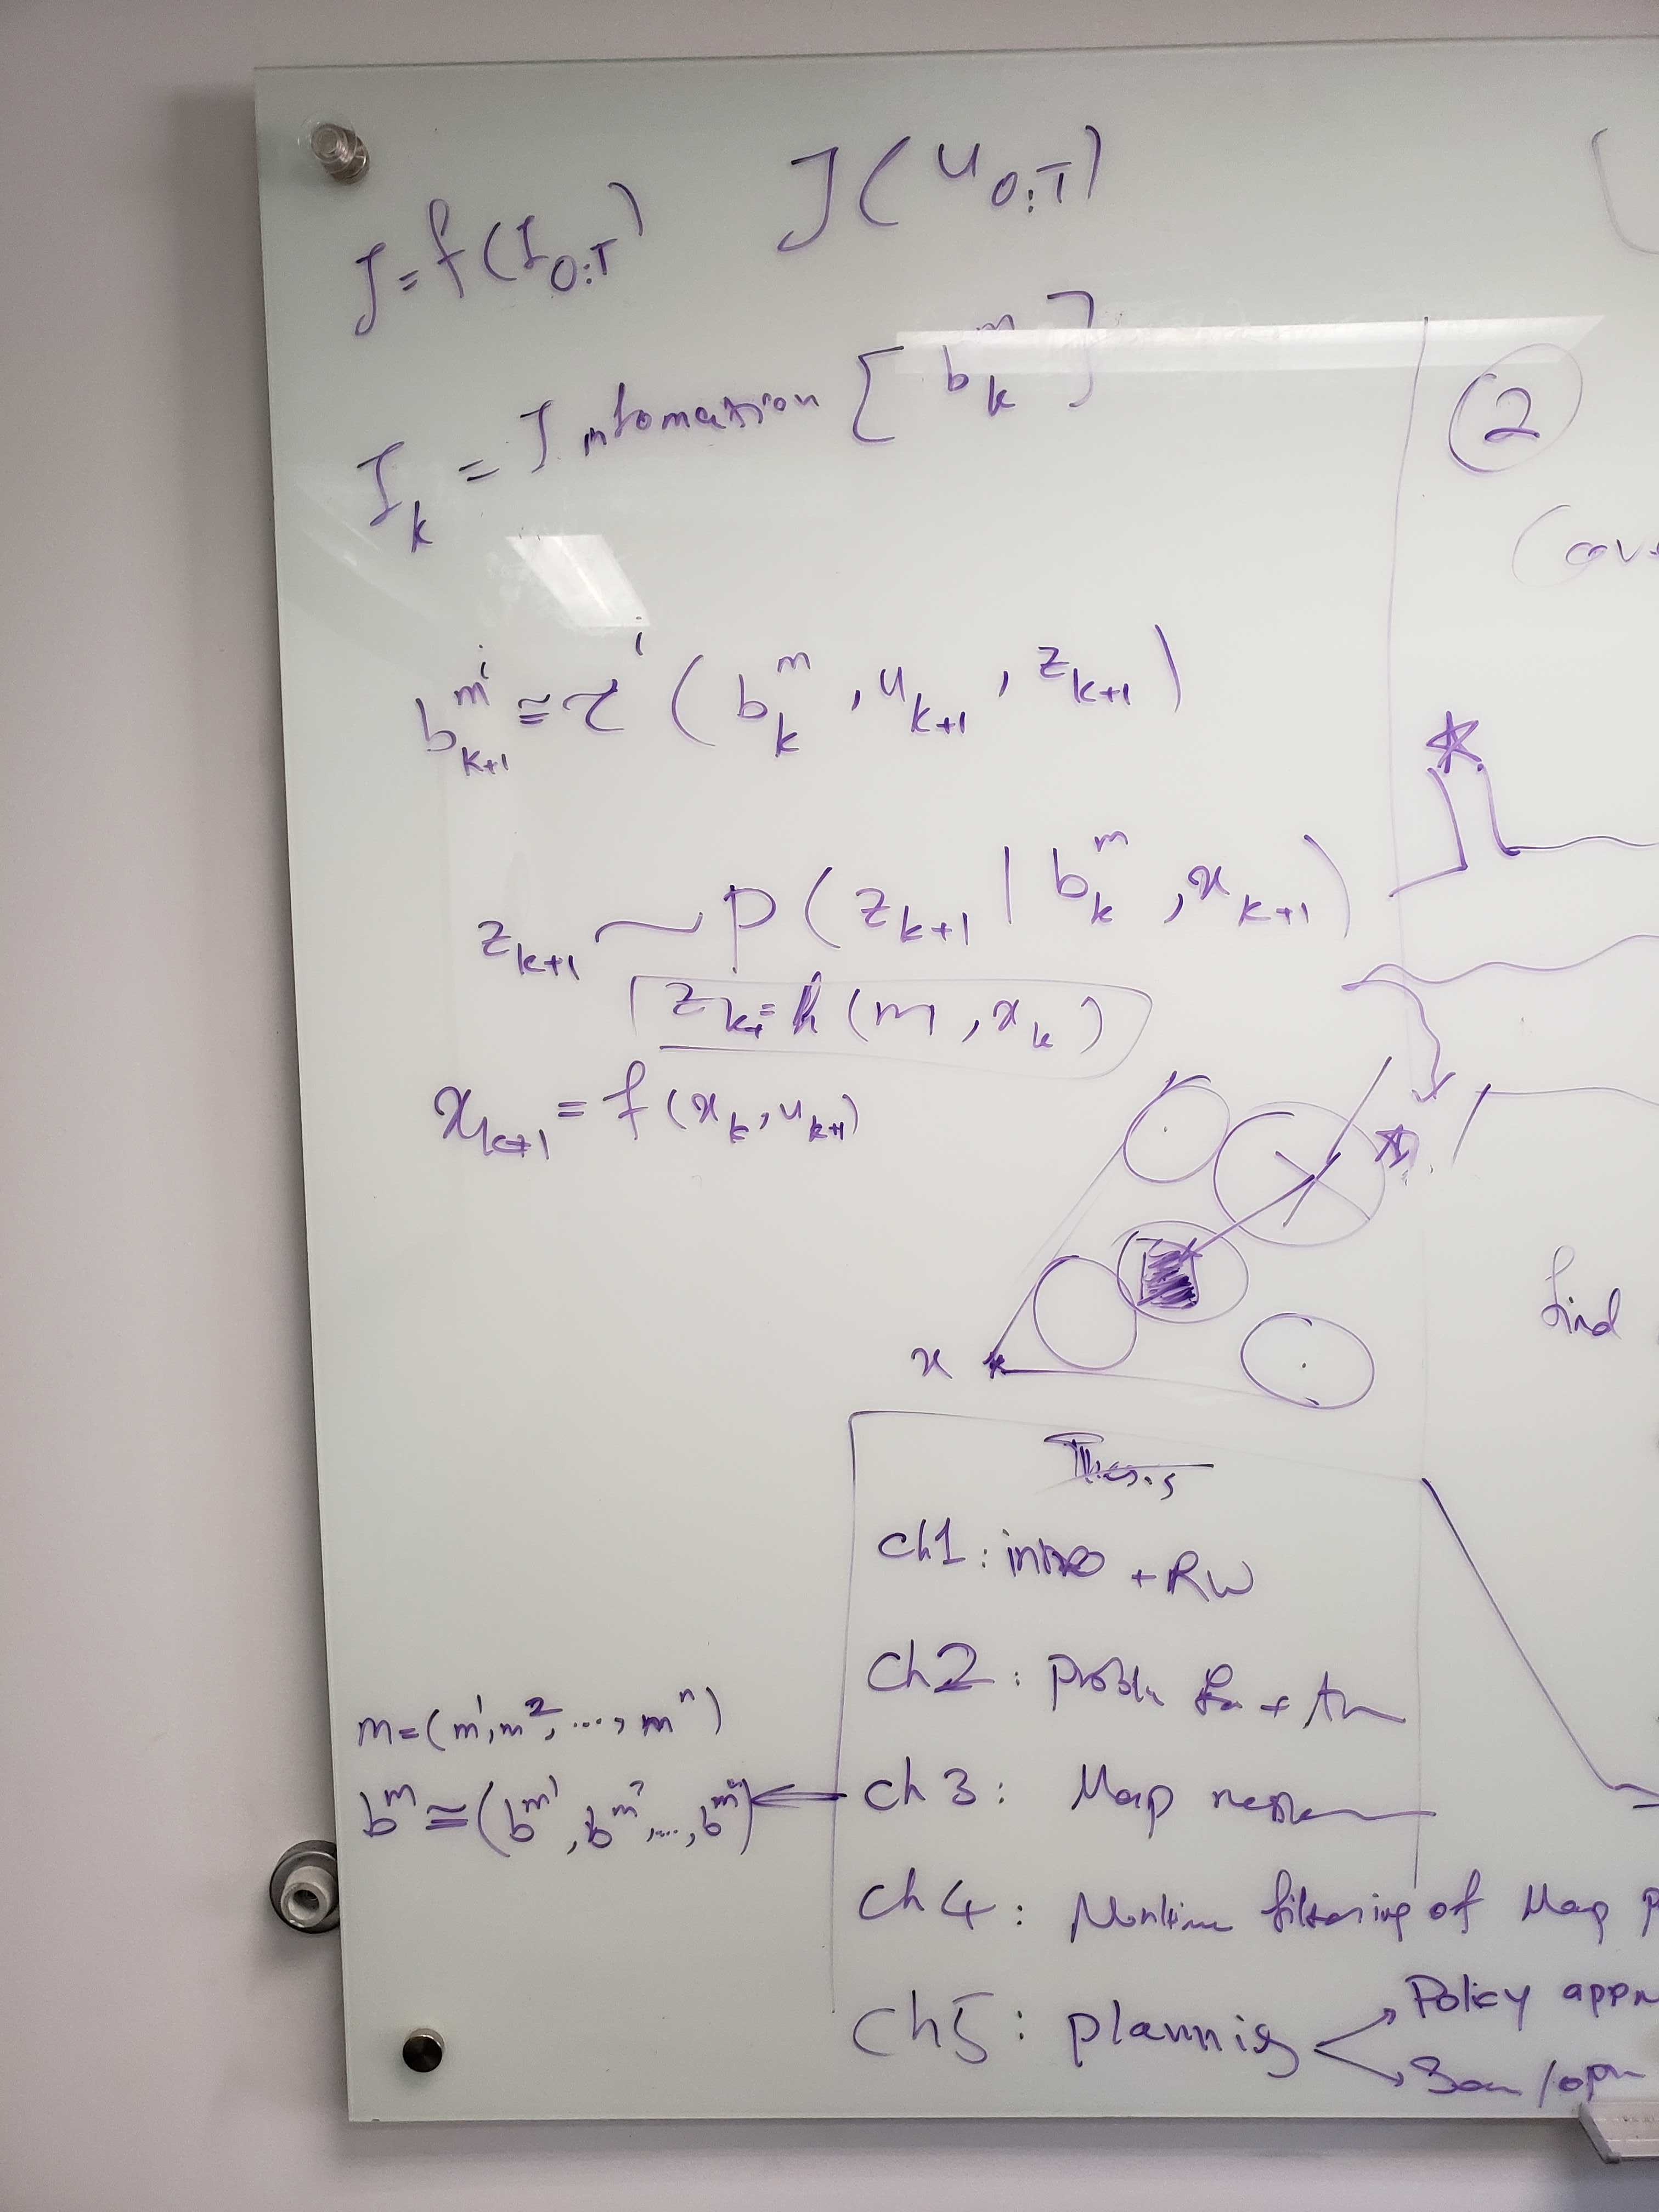
\includegraphics[width=.5\textwidth]{figures/whiteboard2.jpg}
%   \label{fig:whiteboard1}
% \end{figure}

% \begin{figure}[H]
%   \centering
%   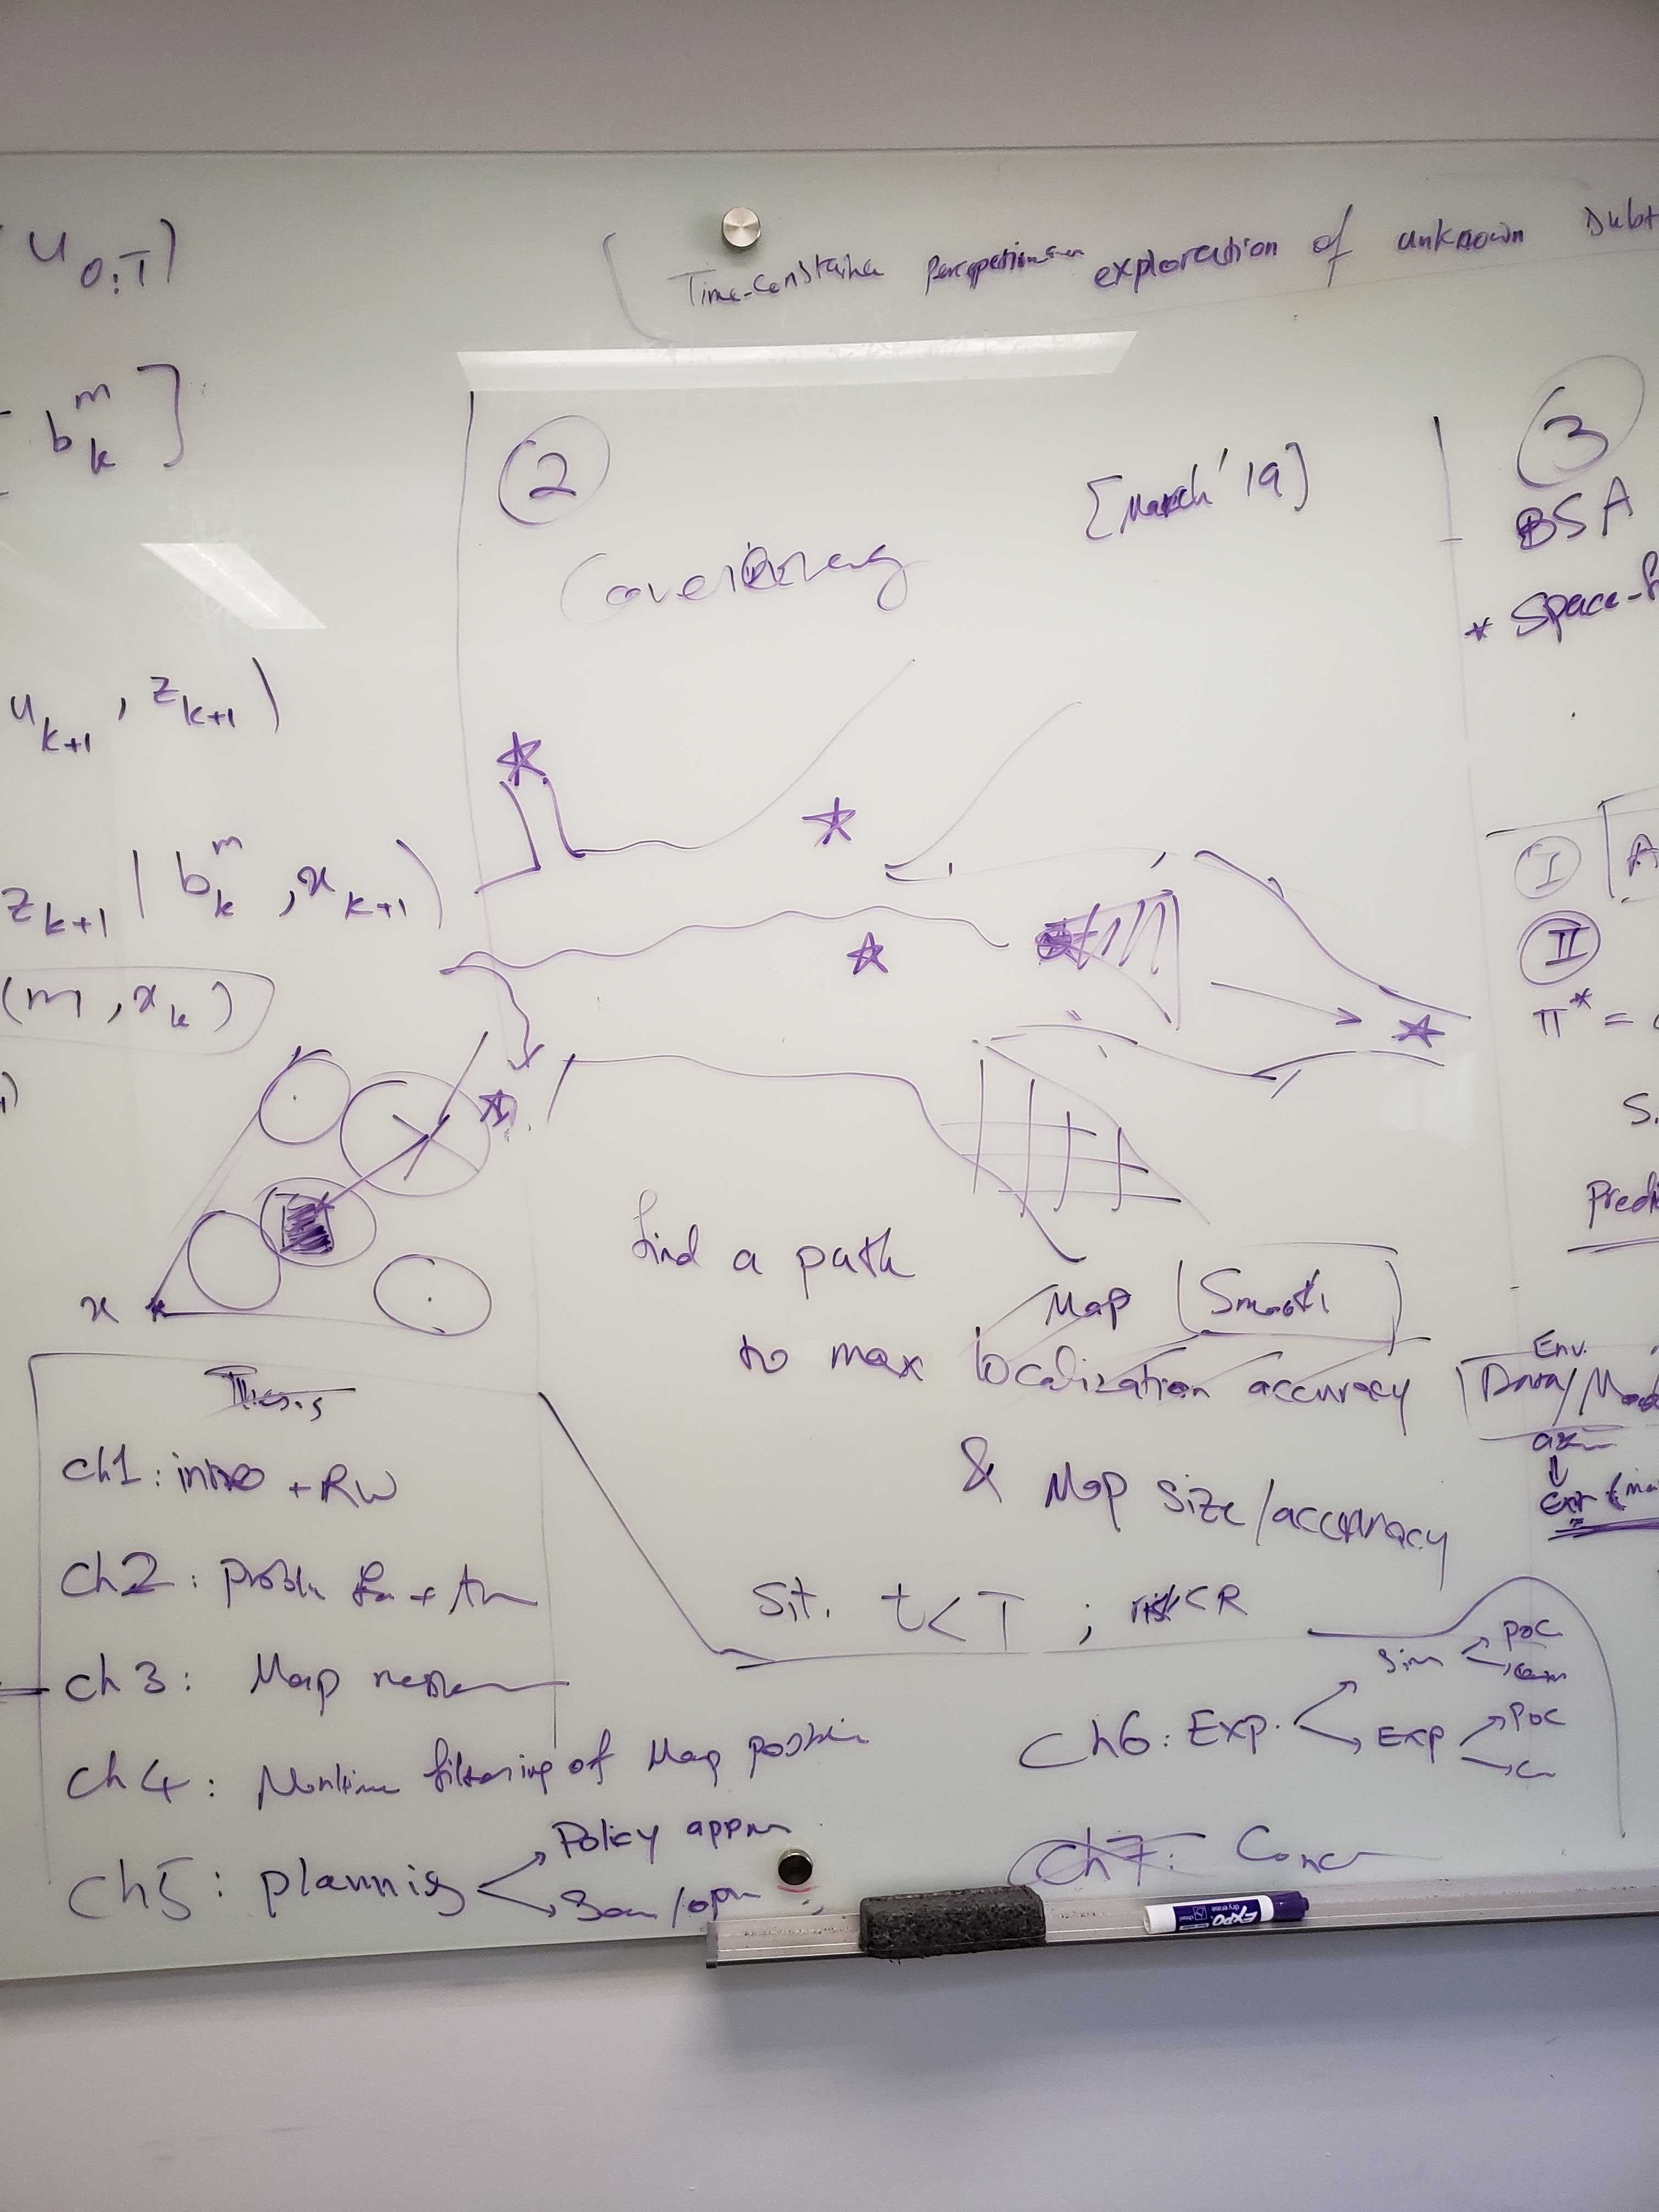
\includegraphics[width=.5\textwidth]{figures/whiteboard3.jpg}
%   \label{fig:whiteboard1}
% \end{figure}

% \begin{figure}[H]
%   \centering
%   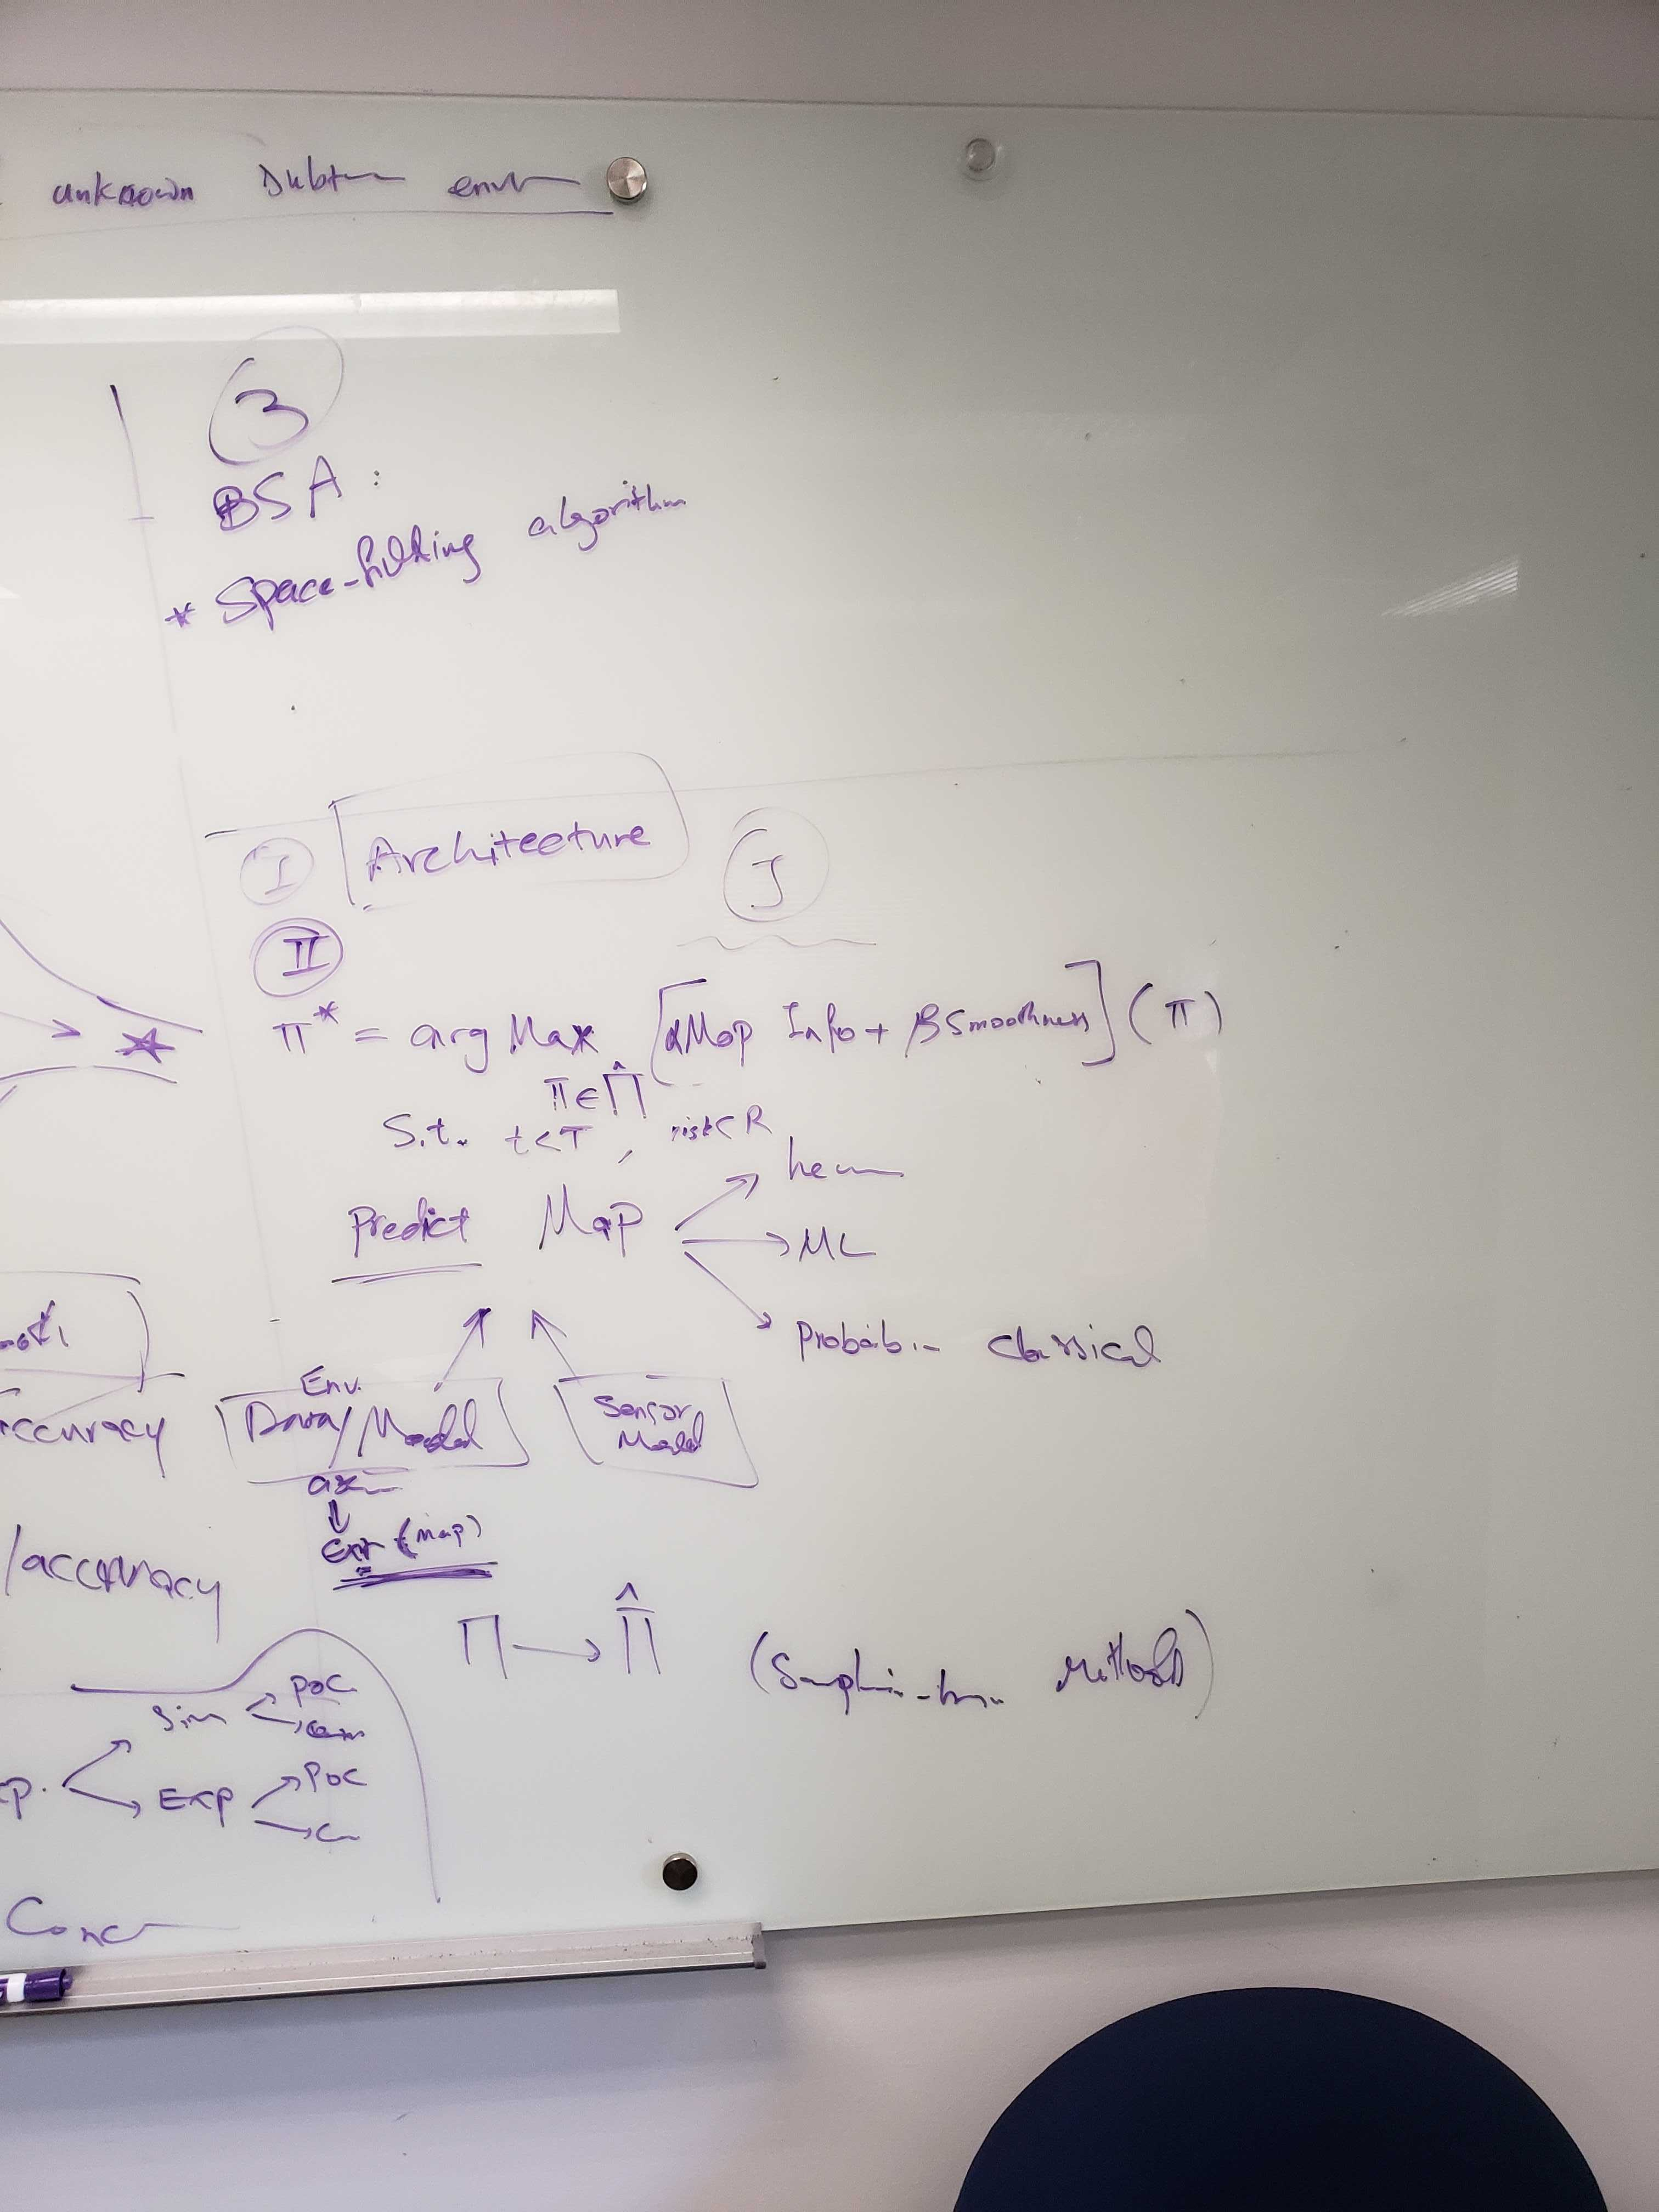
\includegraphics[width=.5\textwidth]{figures/whiteboard4.jpg}
%   \label{fig:whiteboard1}
% \end{figure}

% \clearpage
% \begin{figure}[H]
%   \centering
%   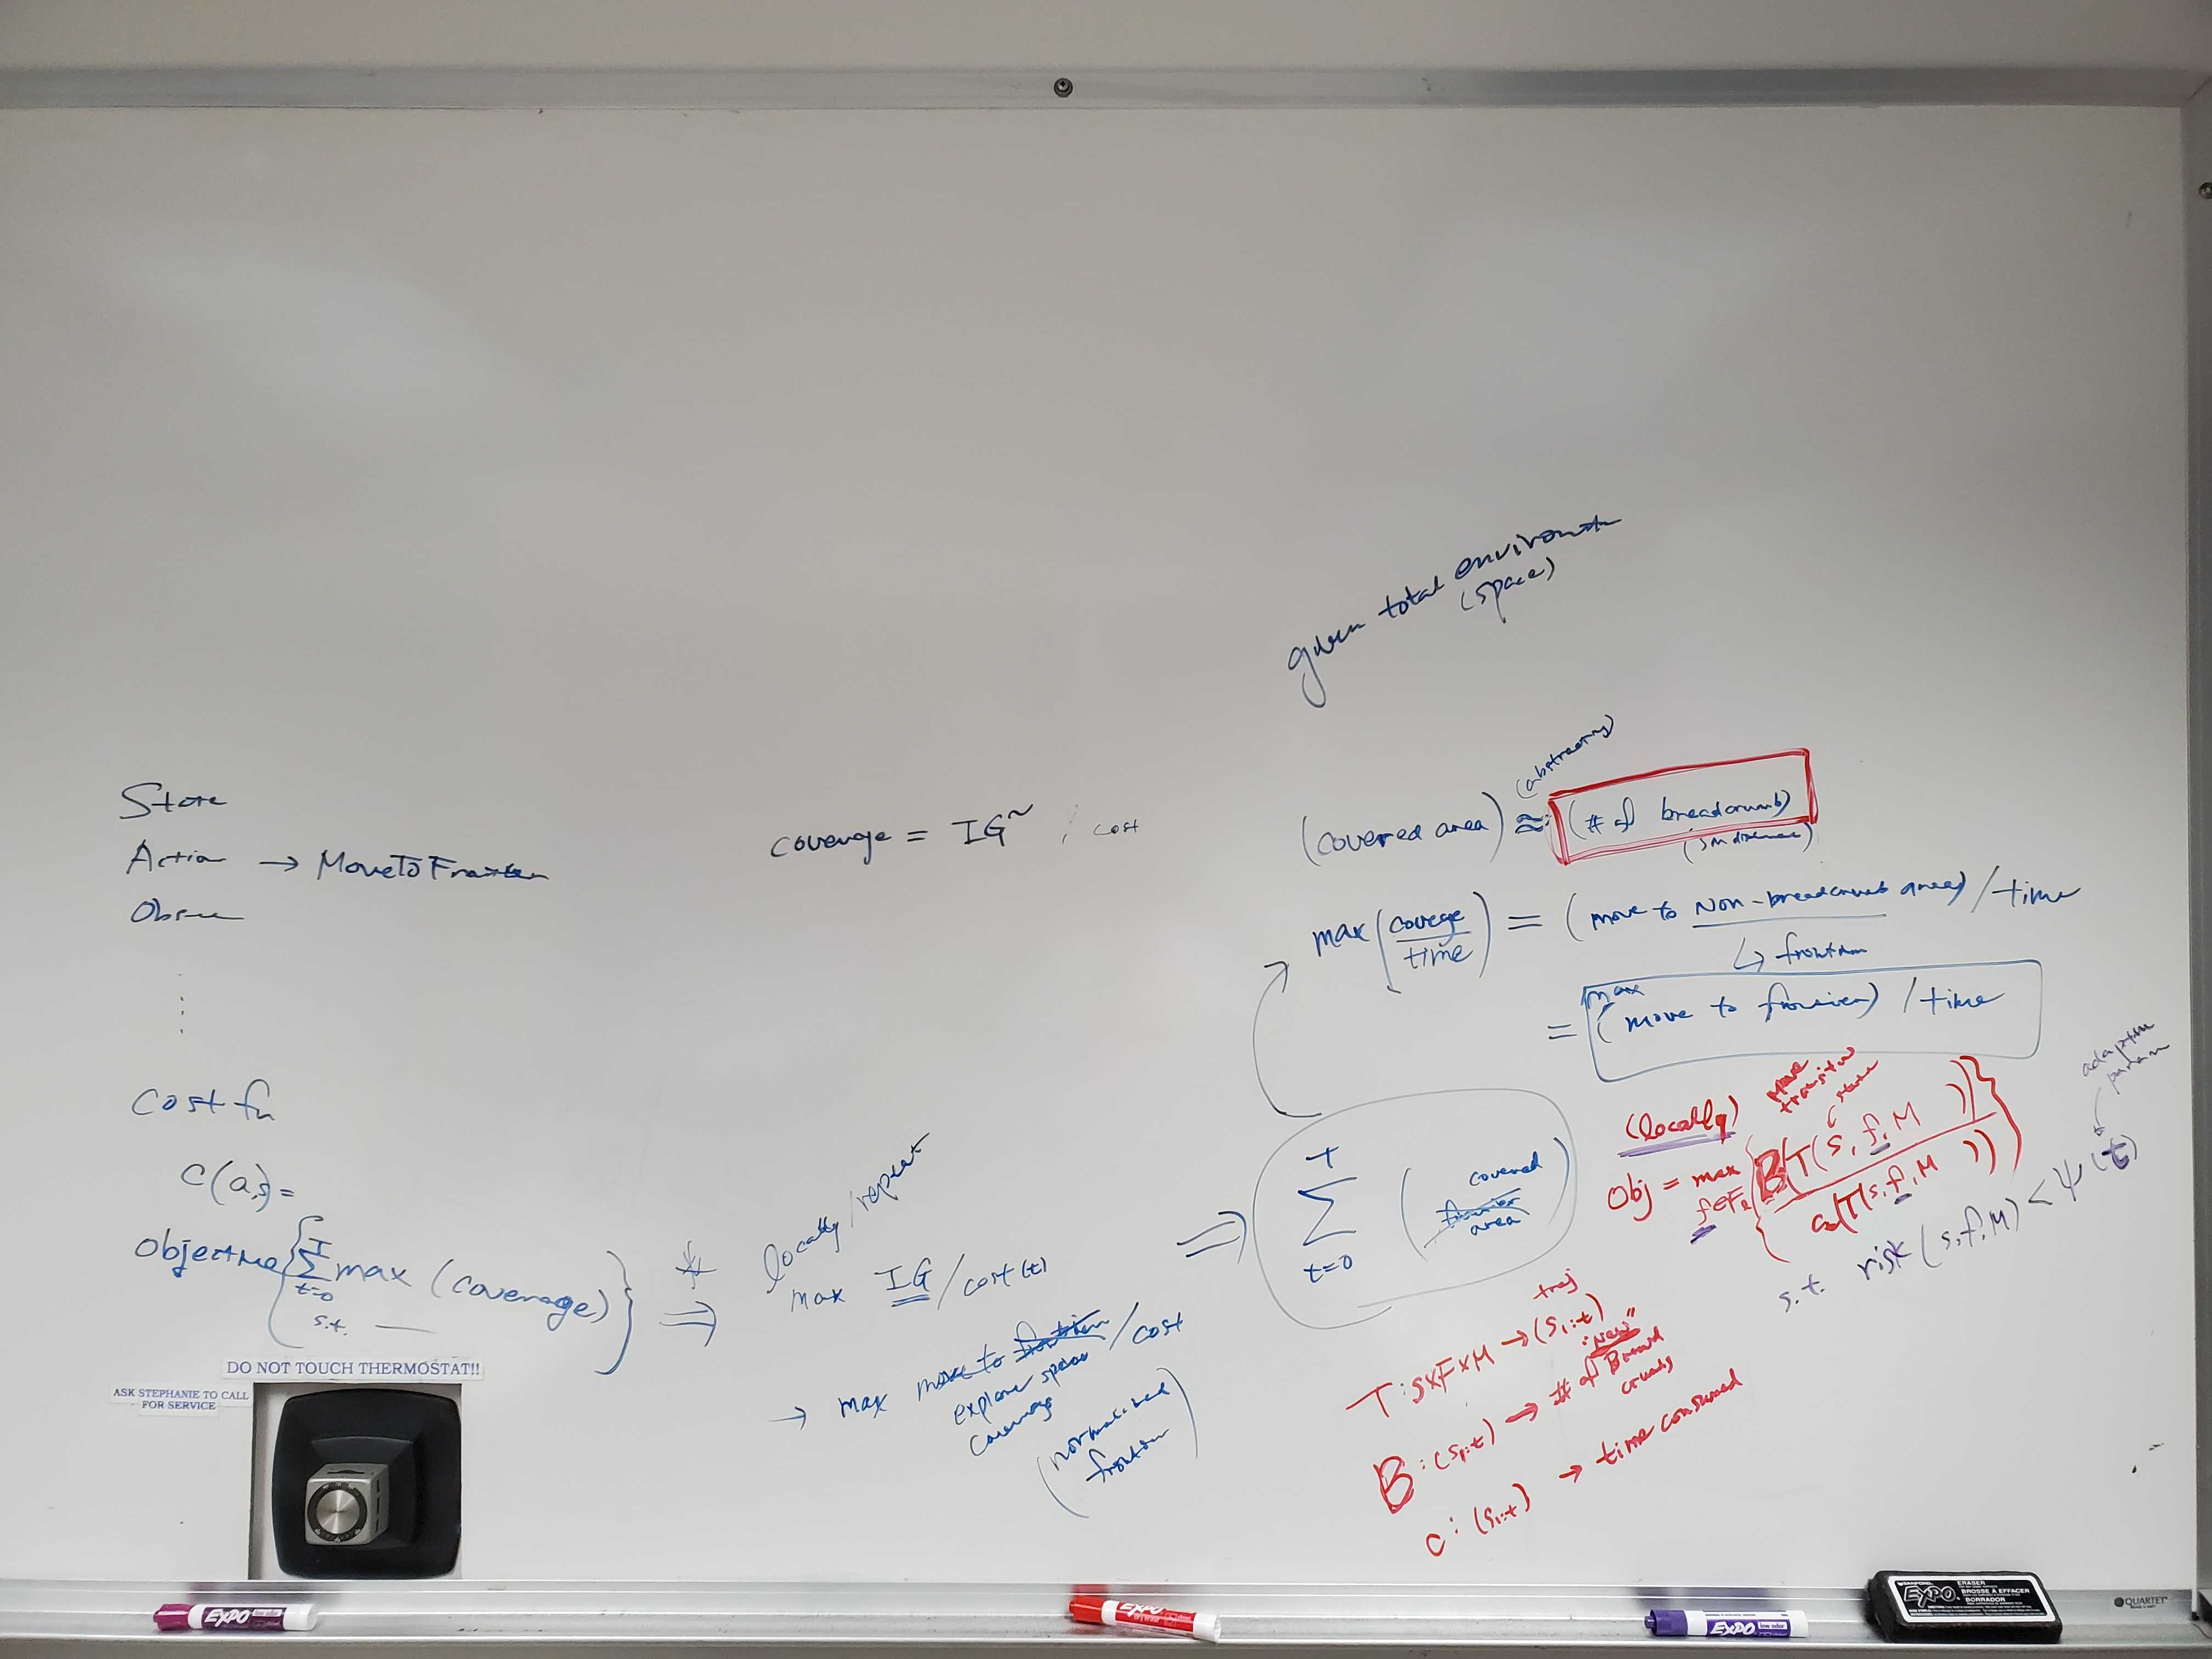
\includegraphics[width=.9\textwidth]{figures/whiteboardA.jpg}
%   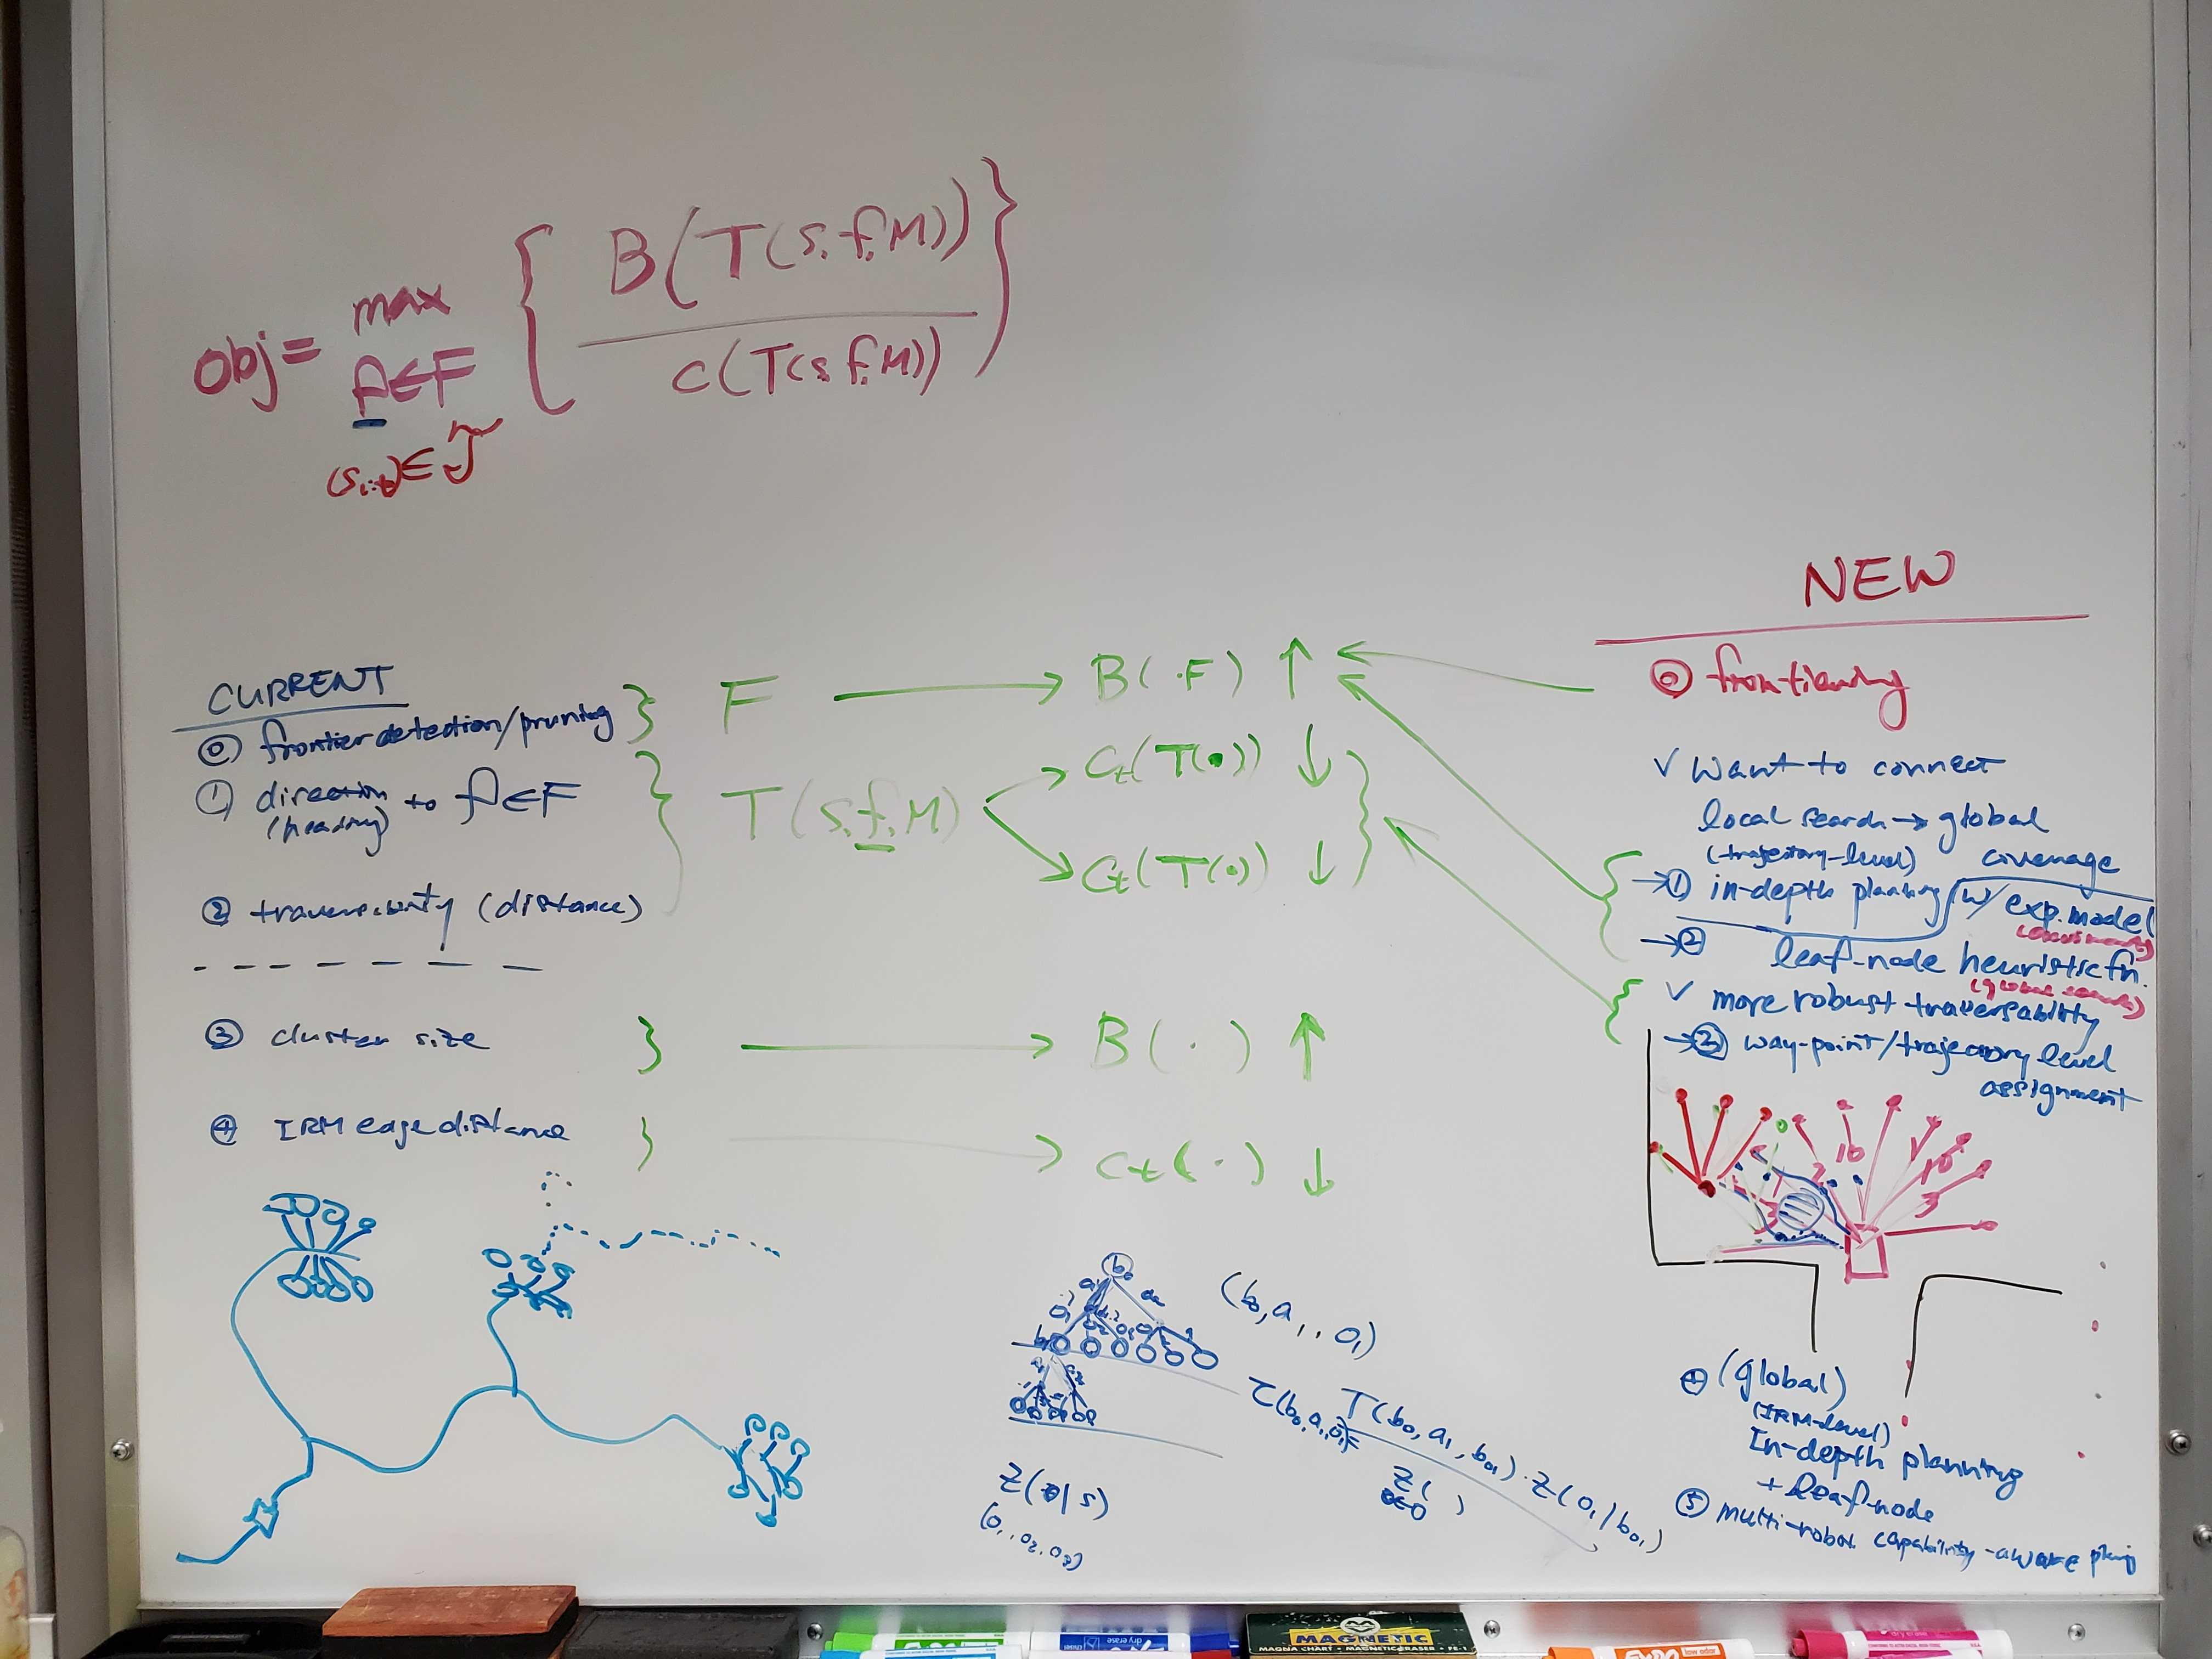
\includegraphics[width=.9\textwidth]{figures/whiteboardB.jpg}
% \end{figure}
% \clearpage

% \clearpage
% \begin{figure}[H]
%   \centering
%   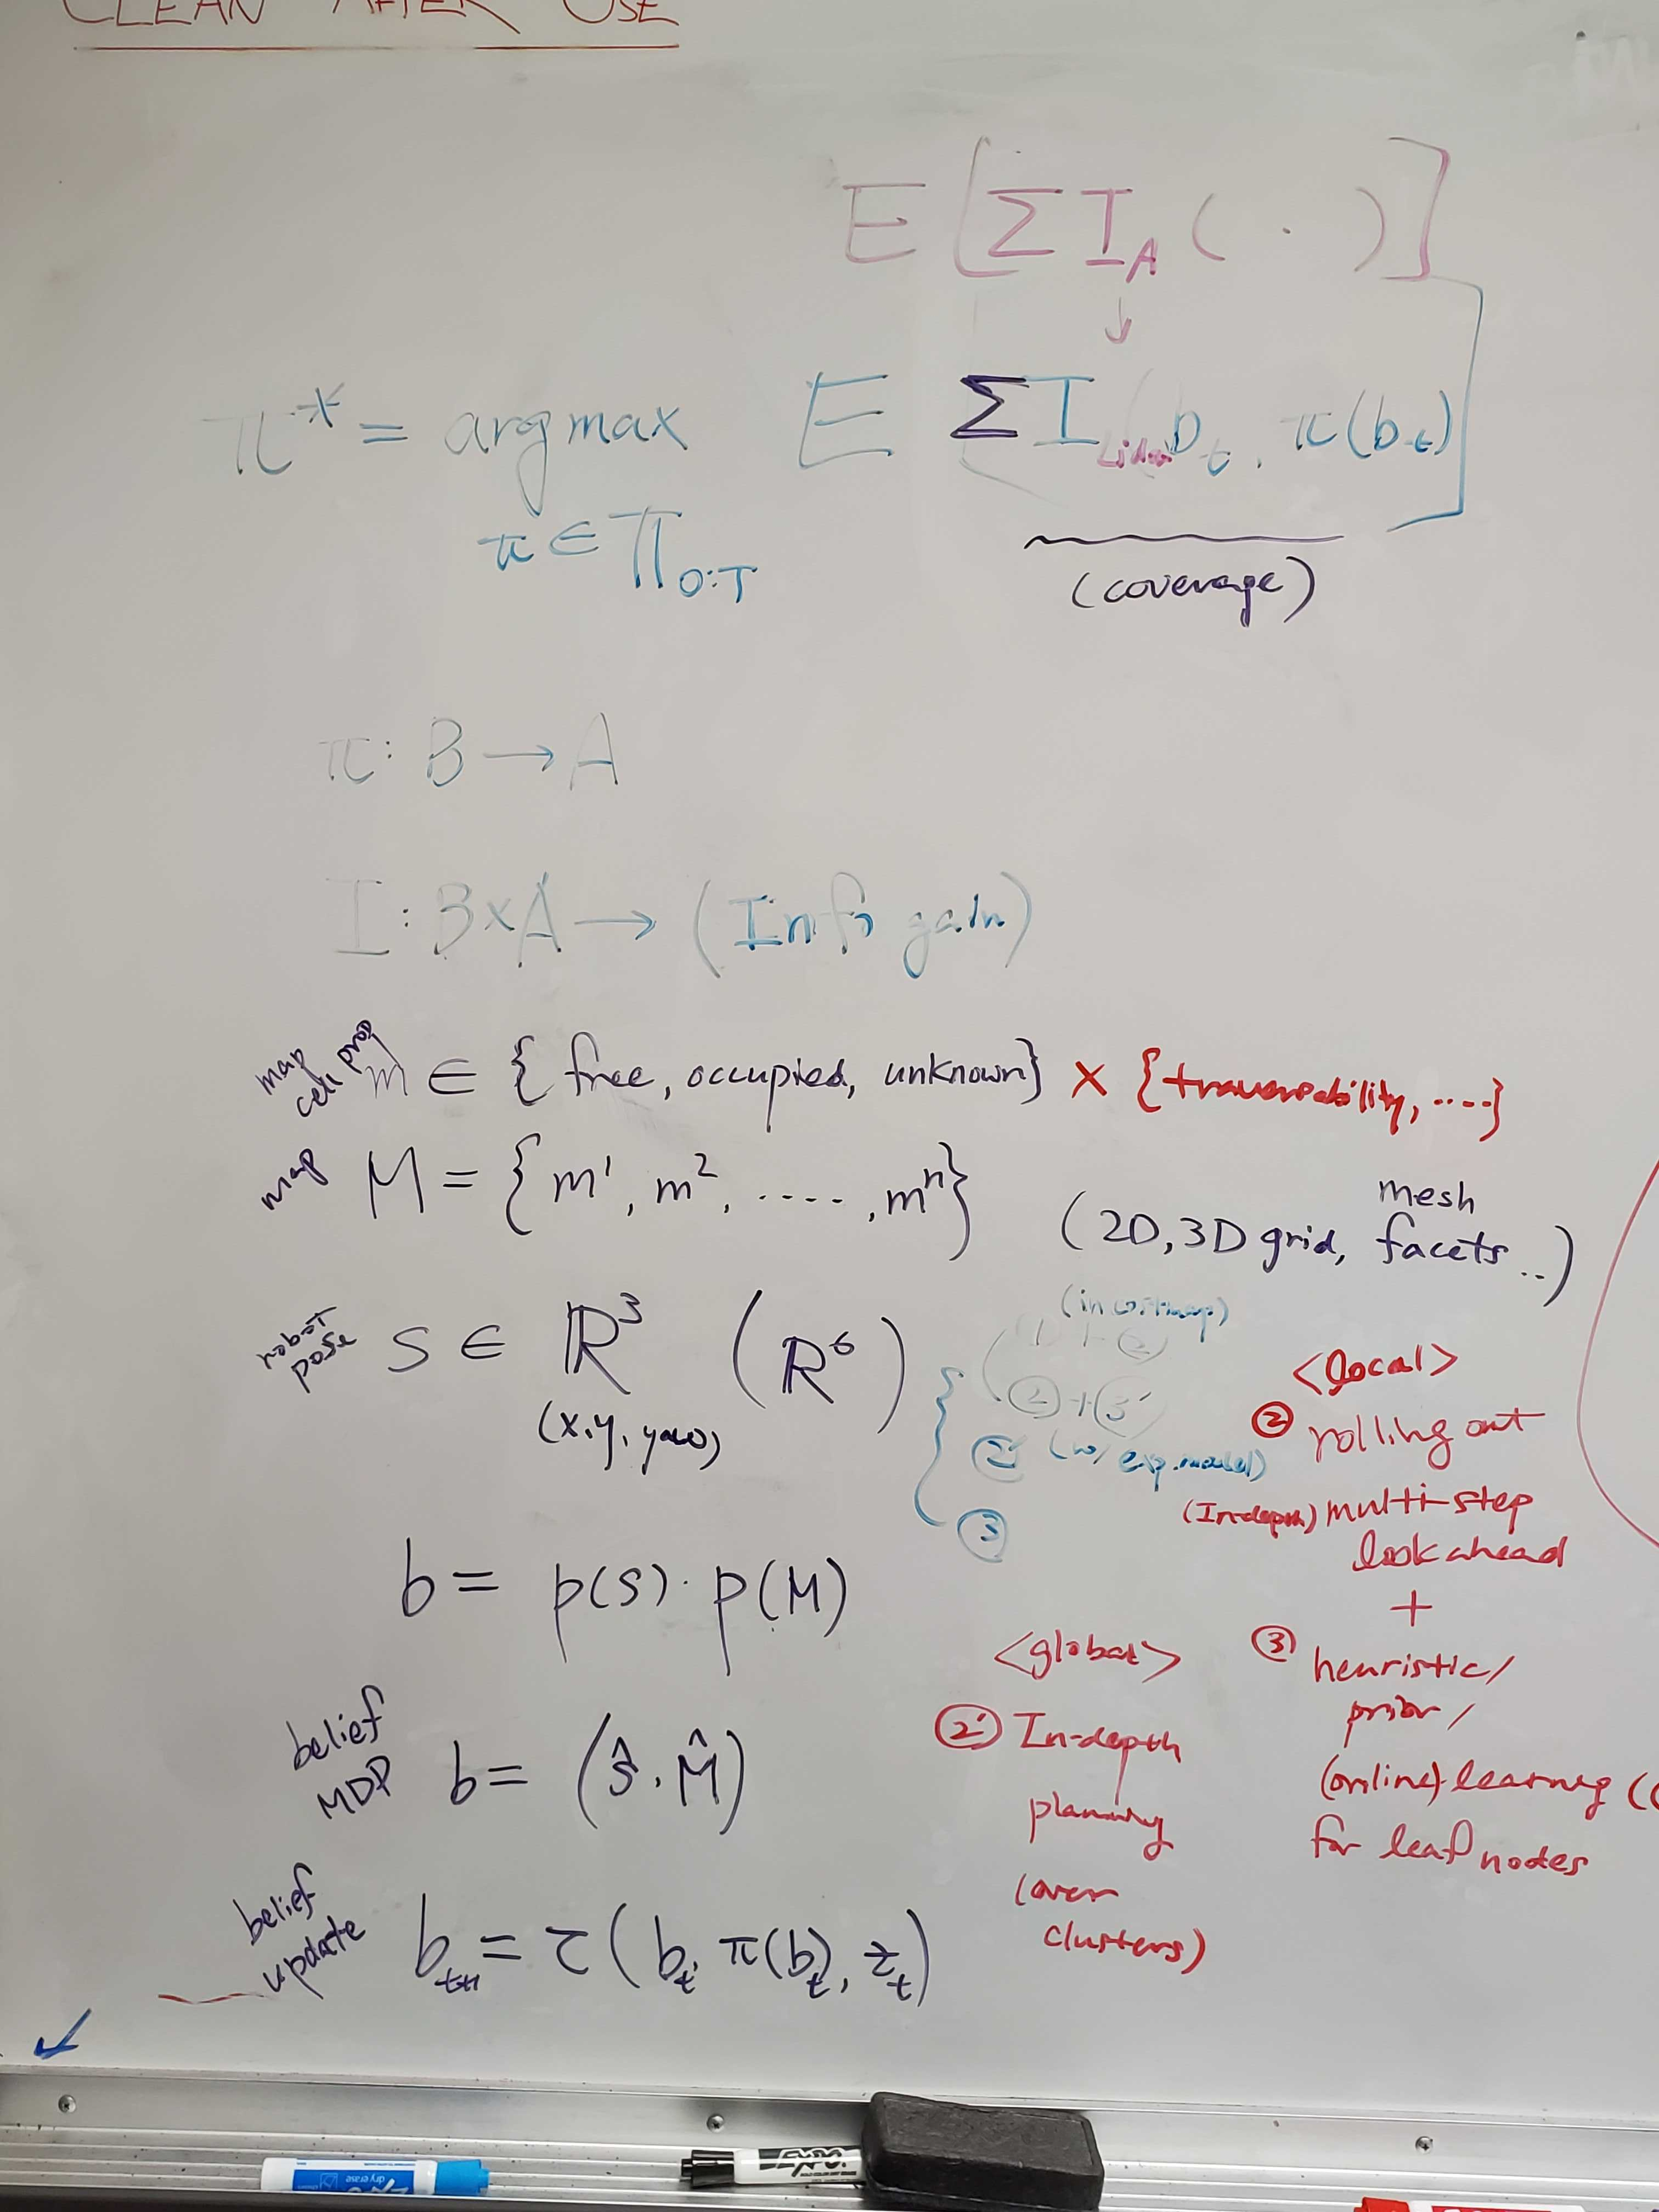
\includegraphics[width=.9\textwidth]{figures/whiteboardI.jpg}
% \end{figure}
% \clearpage
% \begin{figure}[H]
%   \centering
%   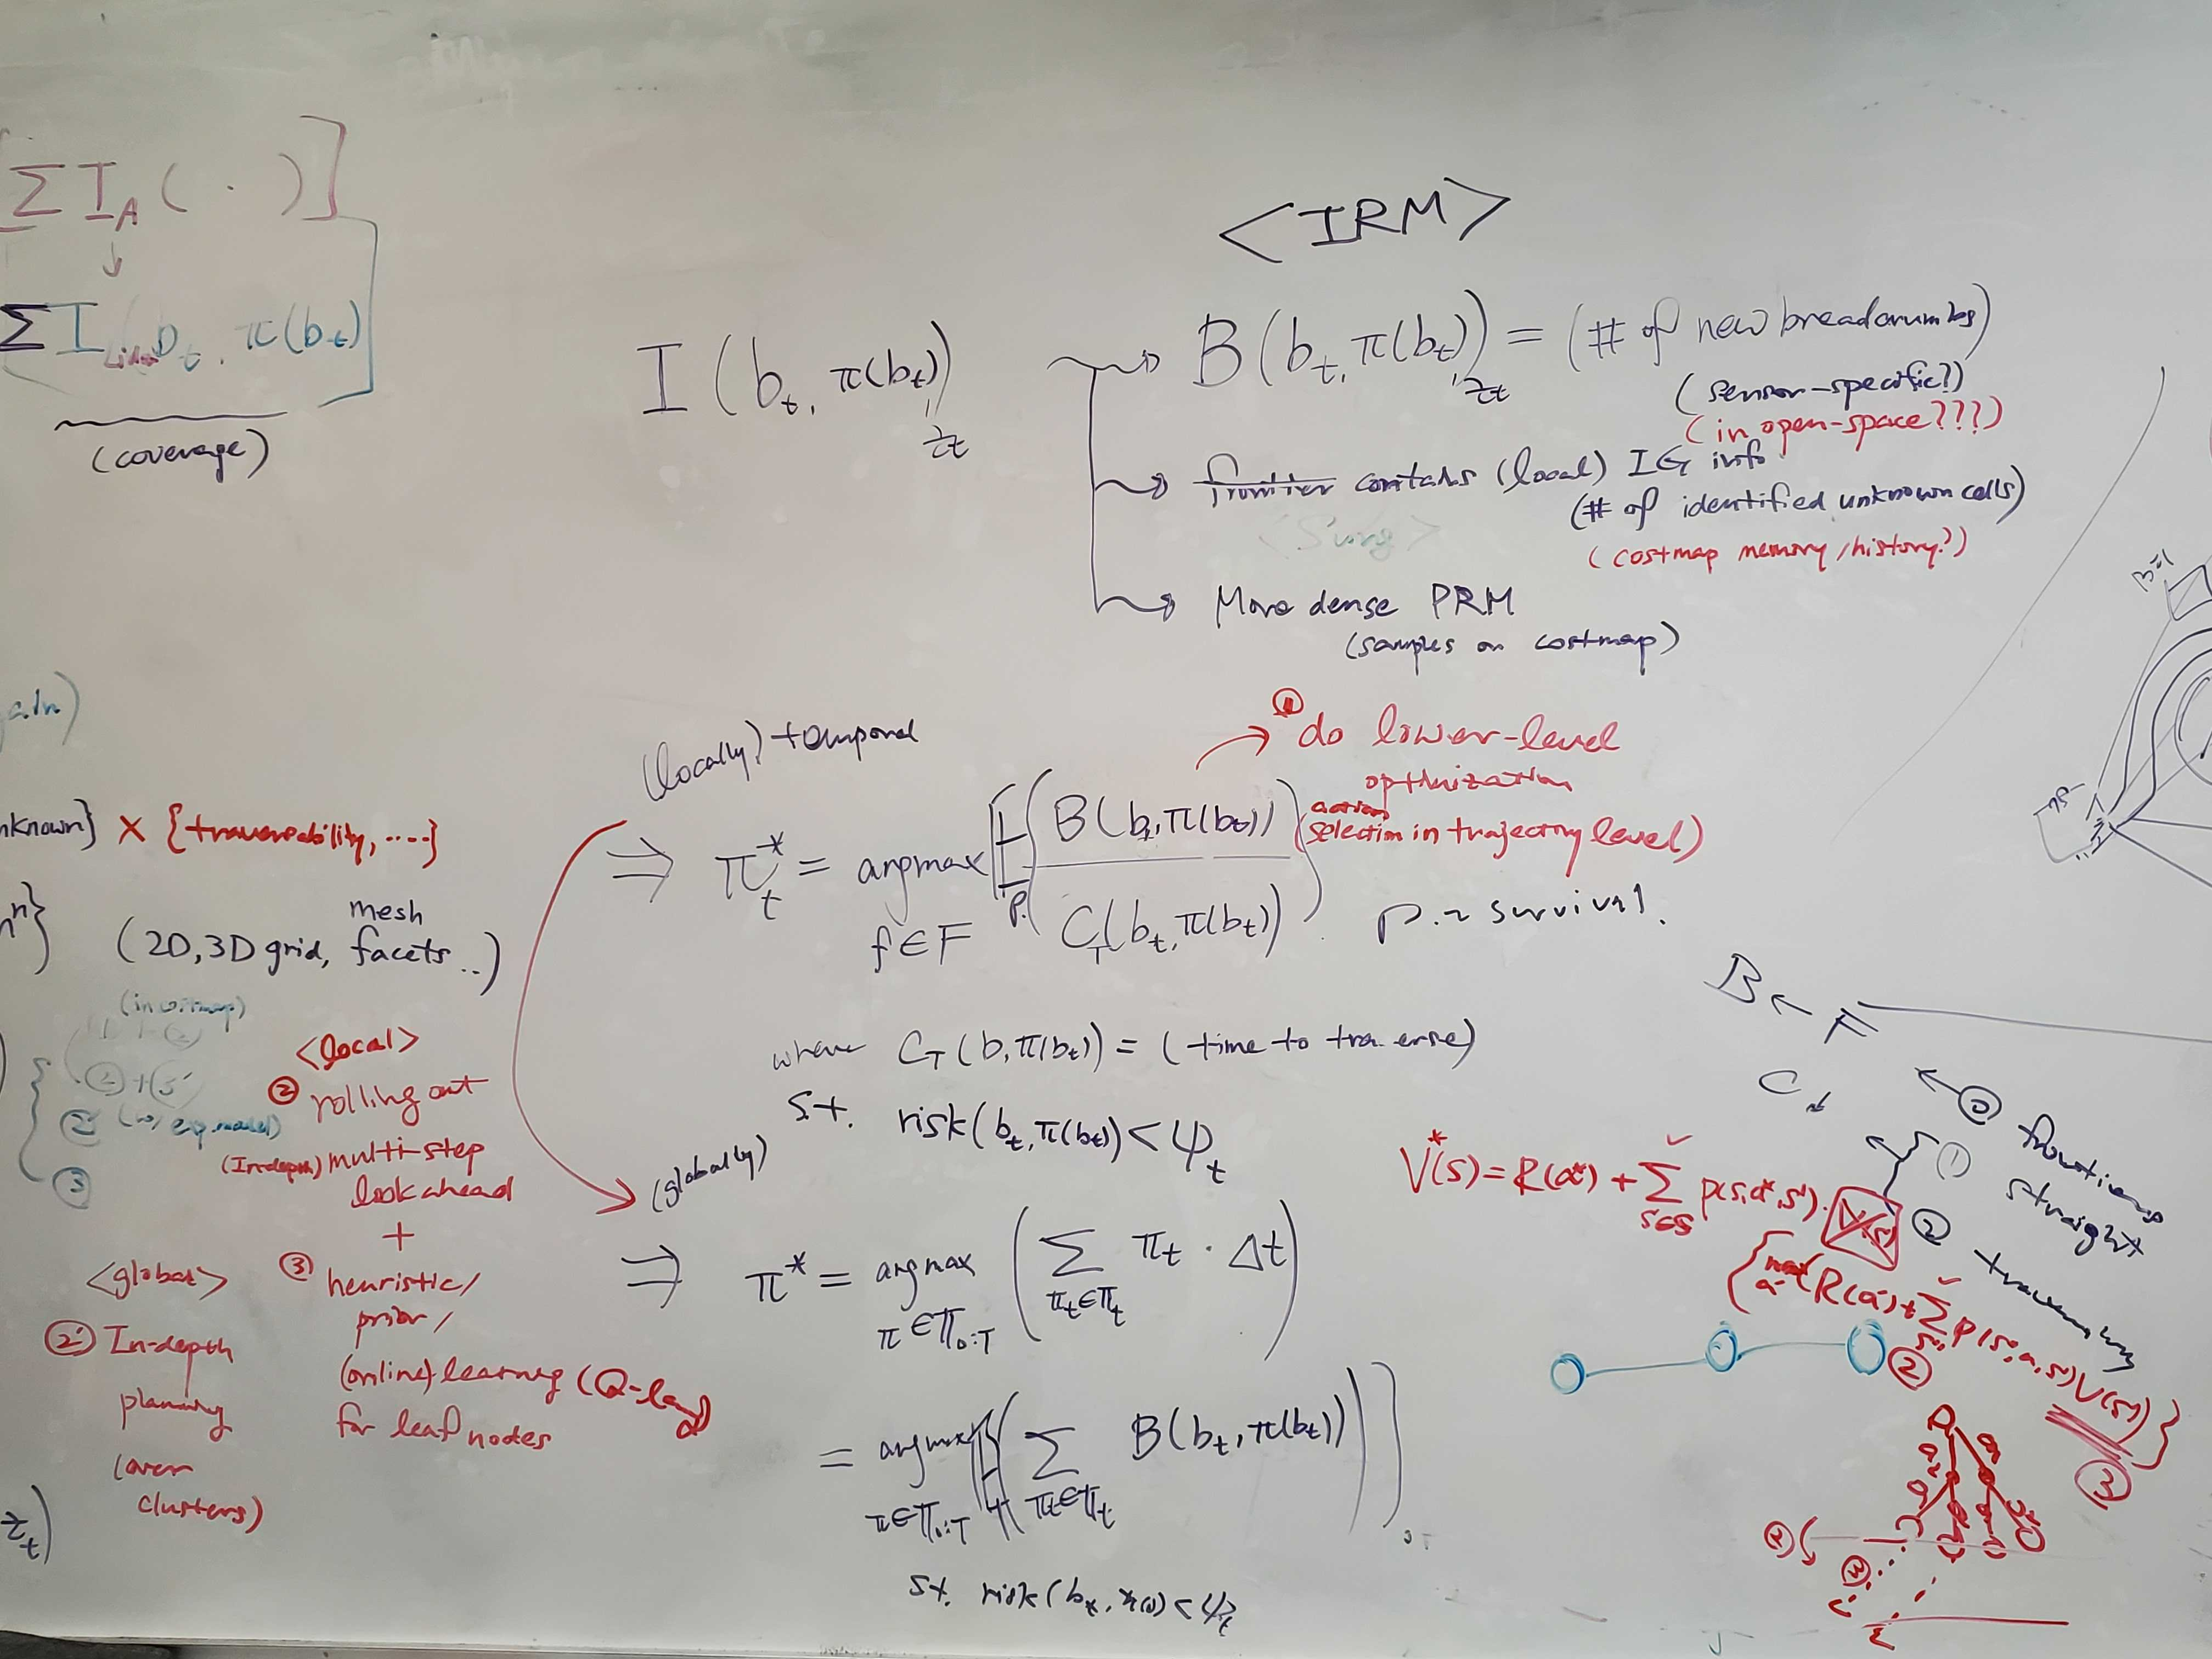
\includegraphics[width=.9\textwidth]{figures/whiteboardII.jpg}
%   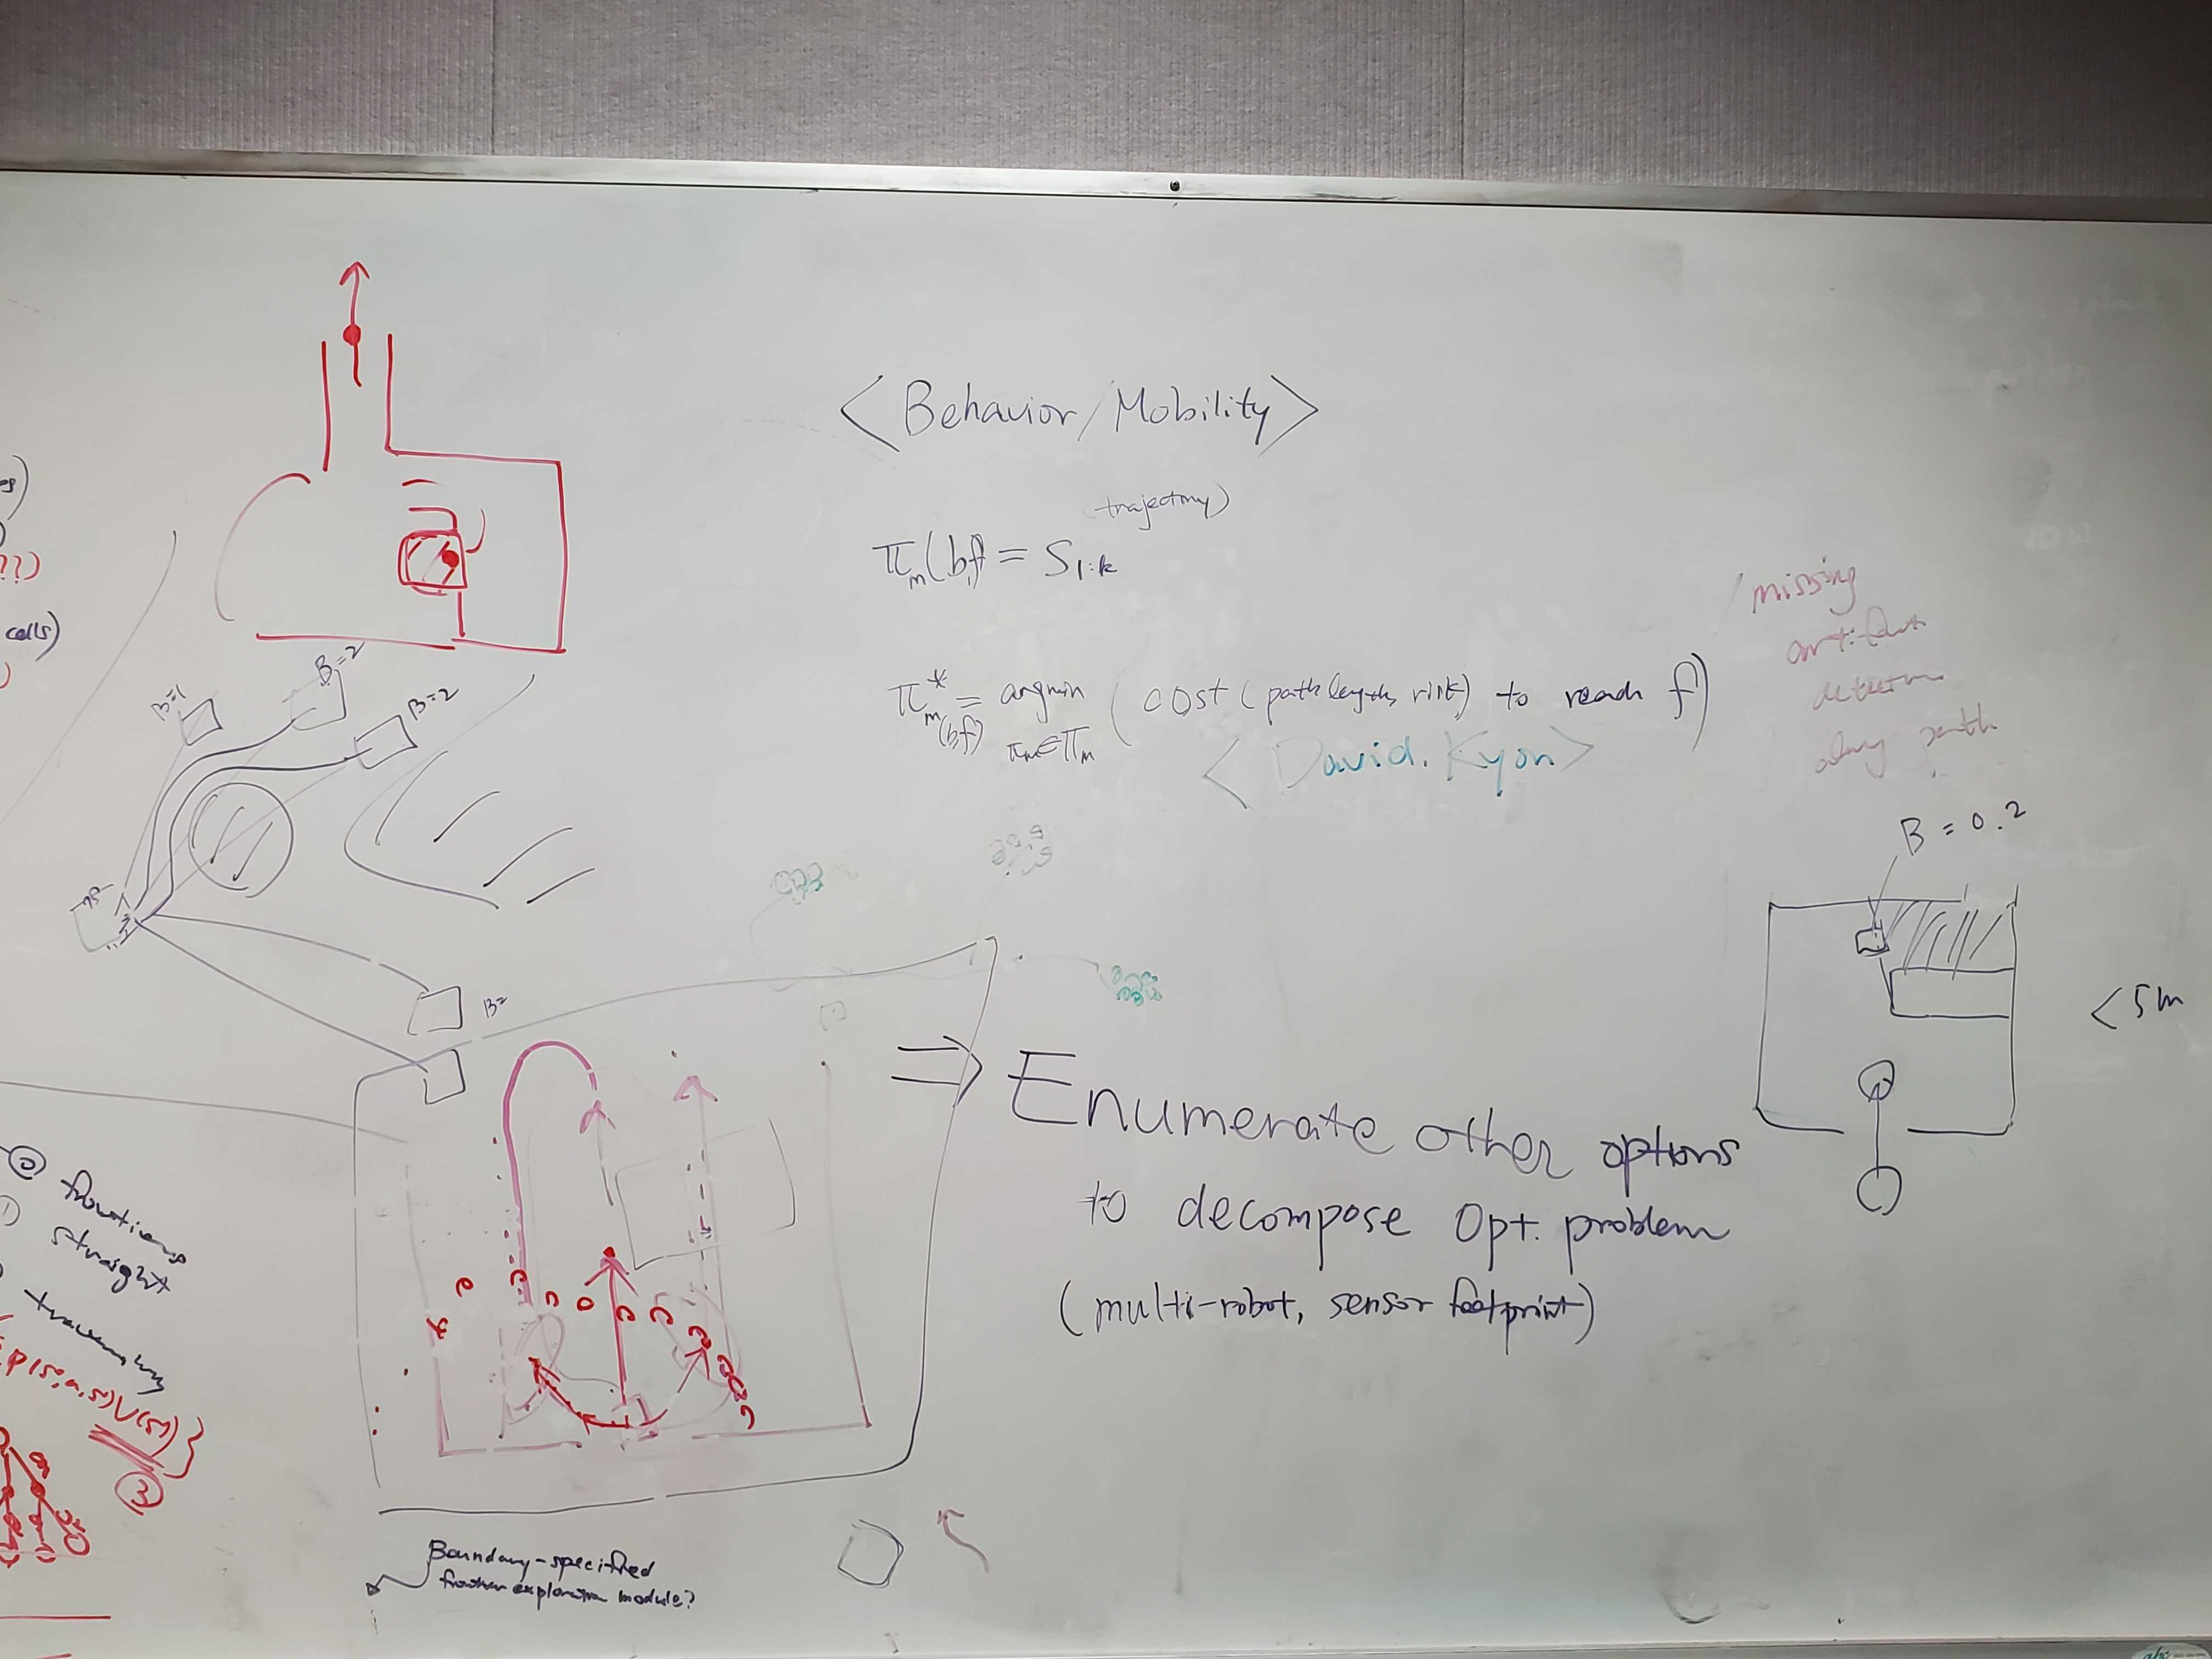
\includegraphics[width=.9\textwidth]{figures/whiteboardIII.jpg}
% \end{figure}
% \clearpage


\end{document}
